\section{Bin Migration Effects}

Upon introduction of a binning scheme to the analysis, we incurred several technical issues. Two of these are finite bin effects and bin volume corrections, which were addressed in \secref{sec:Ch4_corr_factors}. A third comes from the implicit assumption of a bin-by-bin analysis that an event observed to belong in bin number \textit{i} truly belongs to that bin - that is to say that the detector response and reconstruction of the system is high enough that the observed kinematics of the event coincide sufficiently closely with the event's true kinematics as to negligibly change binning variable values. This is only strictly true in the ideal limit of perfect detectors and reconstruction algorithms.

Deviations from the perfect case result in what are known as \textbf{bin migrations}, where an event that truly lies in bin number \textit{i} is instead observed in some other bin \textit{j}. \figref{fig:mig_example} illustrates this effect, which normally only occurs for bins close to a bin edge and results in migration to an adjacent bin, unless bin volumes are very small relative to reconstruction precision.  

\begin{figure}[H]
    \centering
    \subfloat[Reconstructed simulated events in a particular four dimensional bin, shown in its $x_B-Q^2$ bin (left) and t-$\phi$ bin (right).]{%
        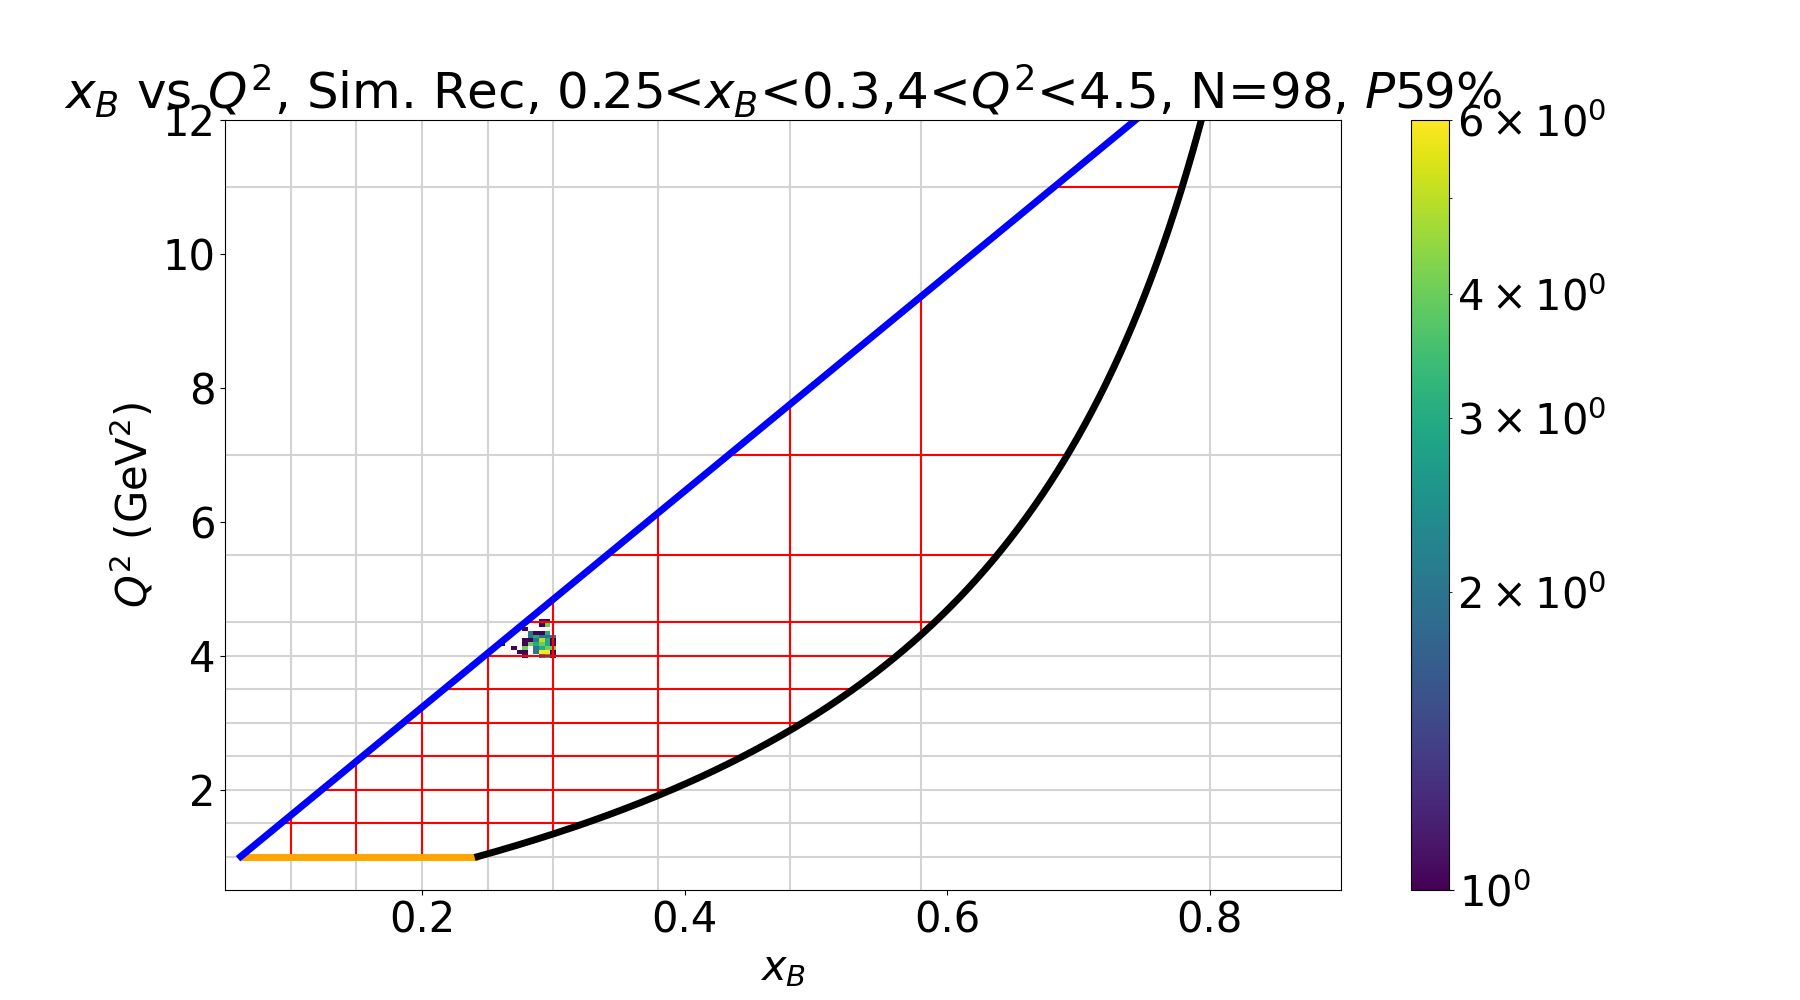
\includegraphics[trim={0 0 10cm 3.5cm},clip,width=0.5\textwidth]{Chapters/Ch5-Further/0_IBU/pics/migration_example/x_B_vs_Q2,_Sim_Rec,_025x_B03,4Q245,_N=98,_P59.png}
        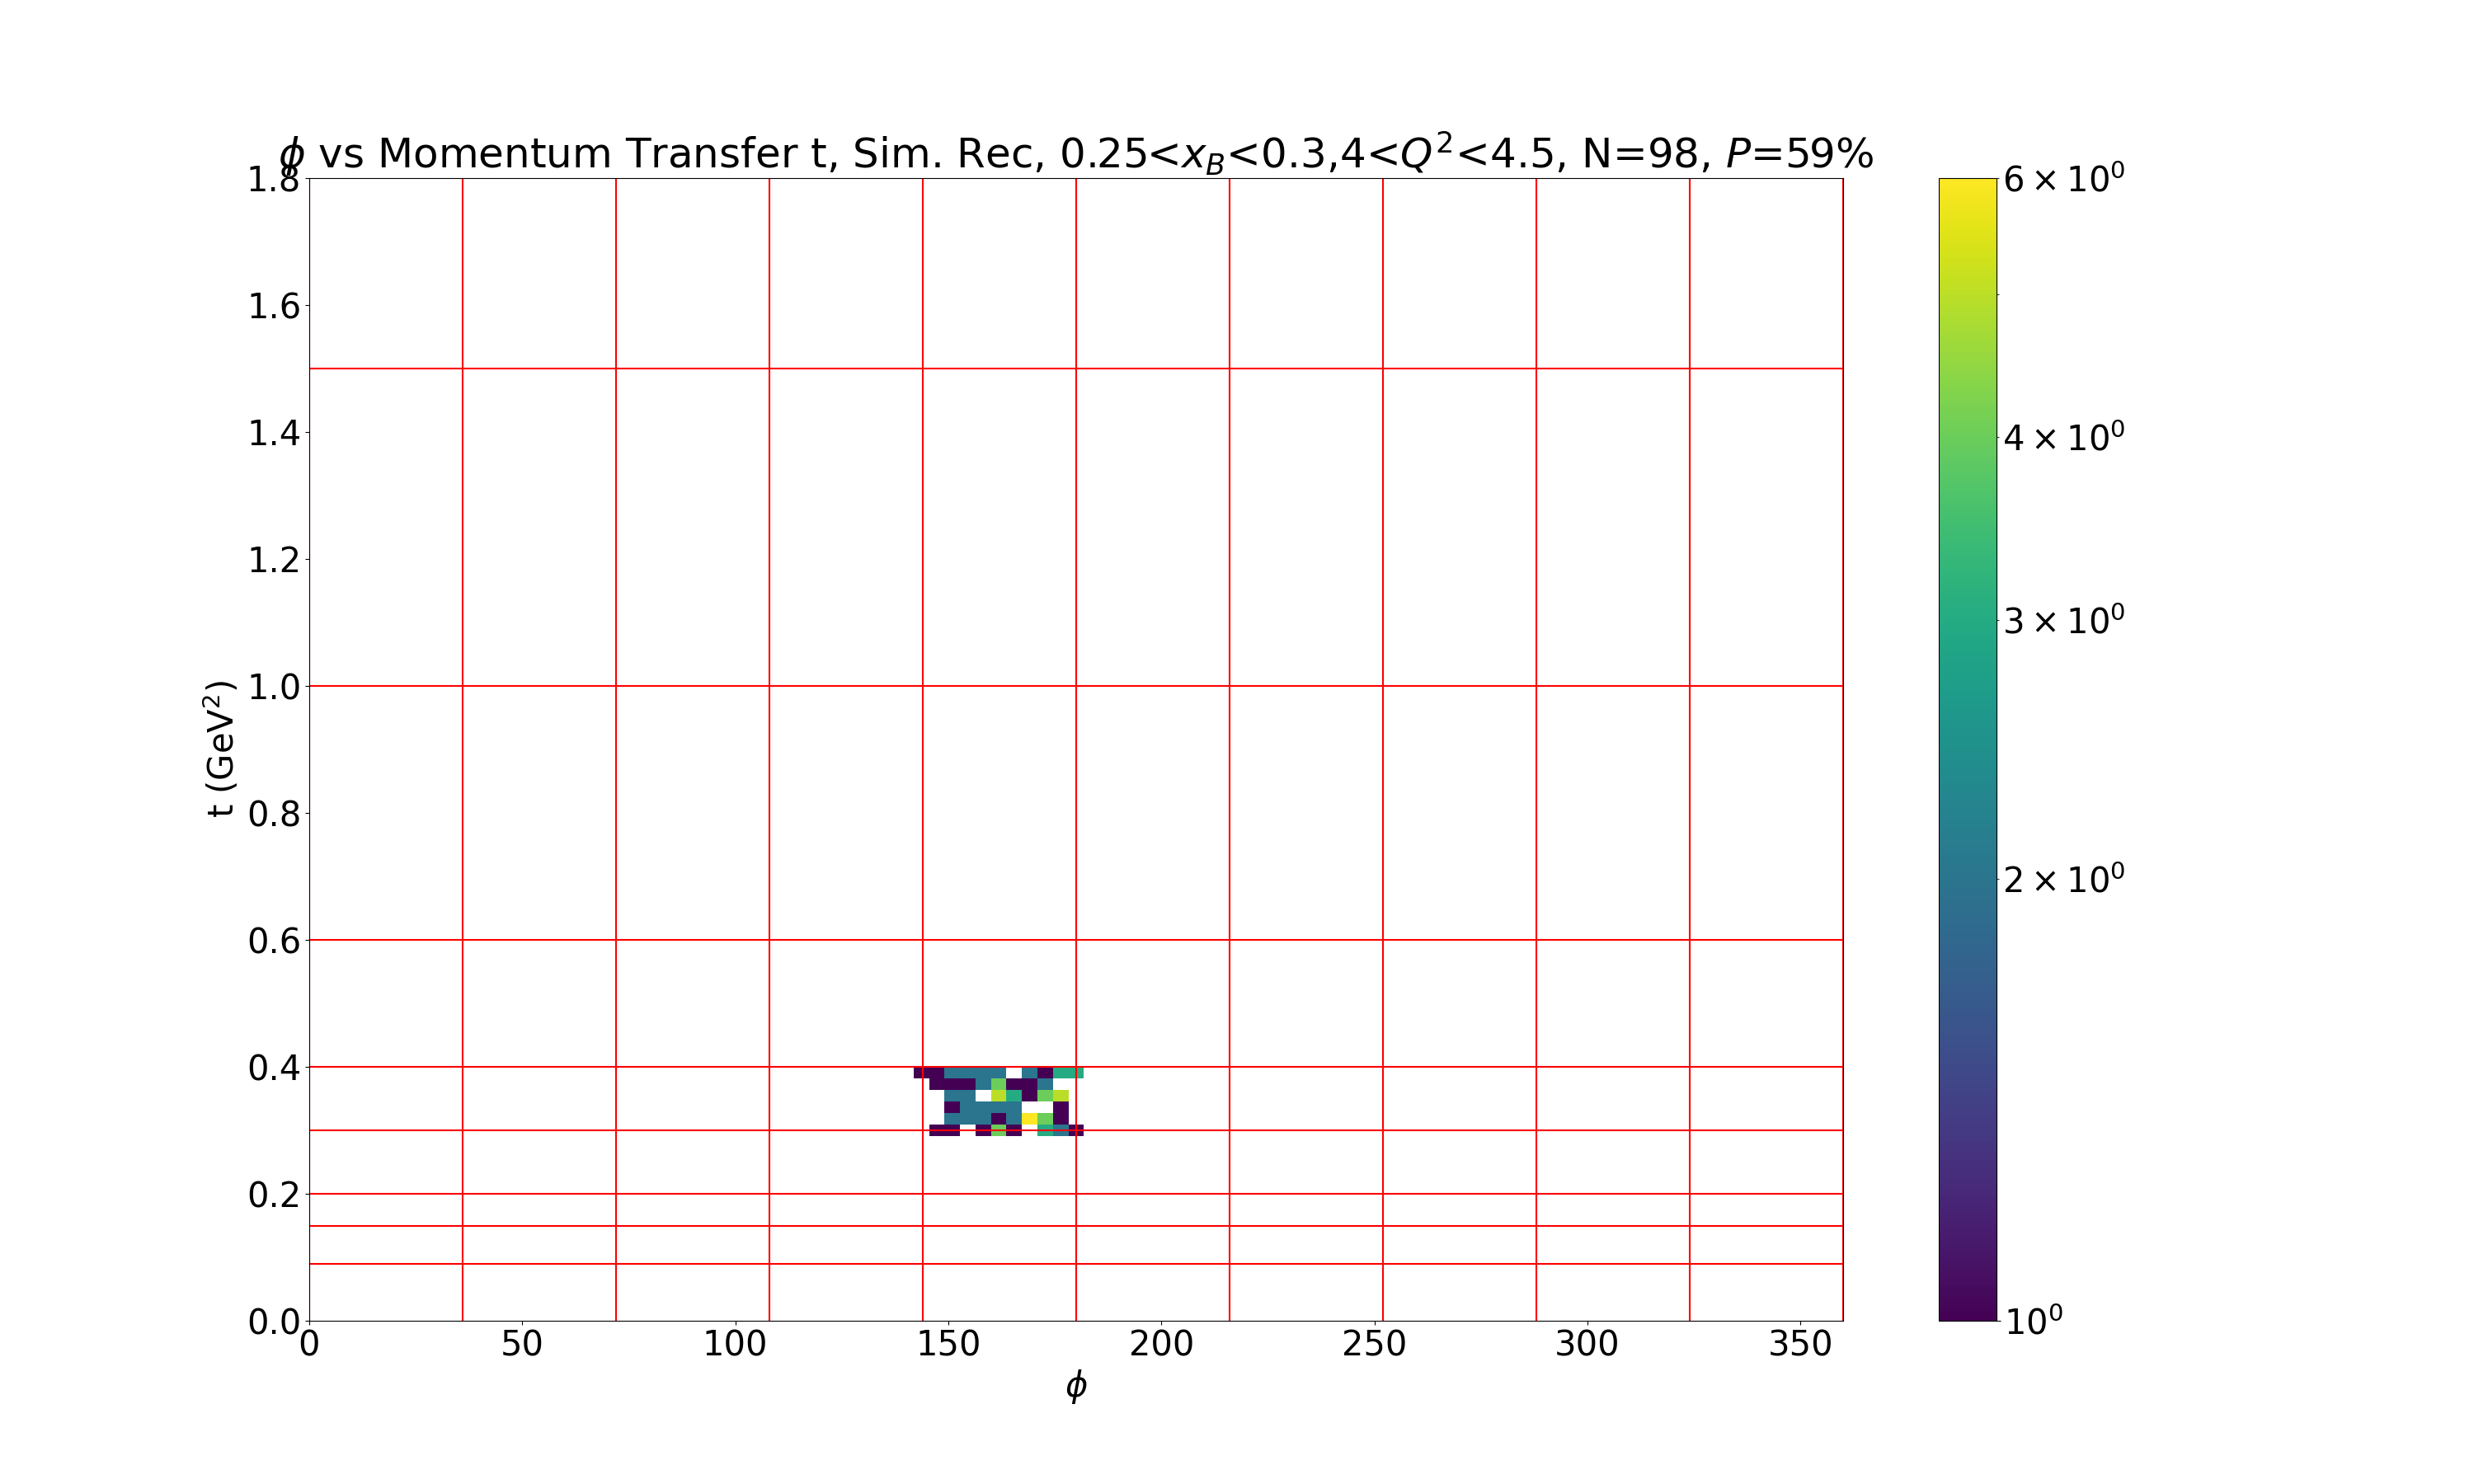
\includegraphics[trim={0 0 17.5cm 6cm},clip,width=0.45\textwidth]{Chapters/Ch5-Further/0_IBU/pics/migration_example/phi_vs_Momentum_Transfer_t,_Sim_Rec,_025x_B03,4Q245,_N=98,_P=59.png}
        \label{fig:reconstructed_events}
    }

    \vspace{1cm}

    \subfloat[Generated simulated (truth) events in a particular four dimensional bin, shown in its $x_B-Q^2$ bin (left) and t-$\phi$ bin (right).]{%
        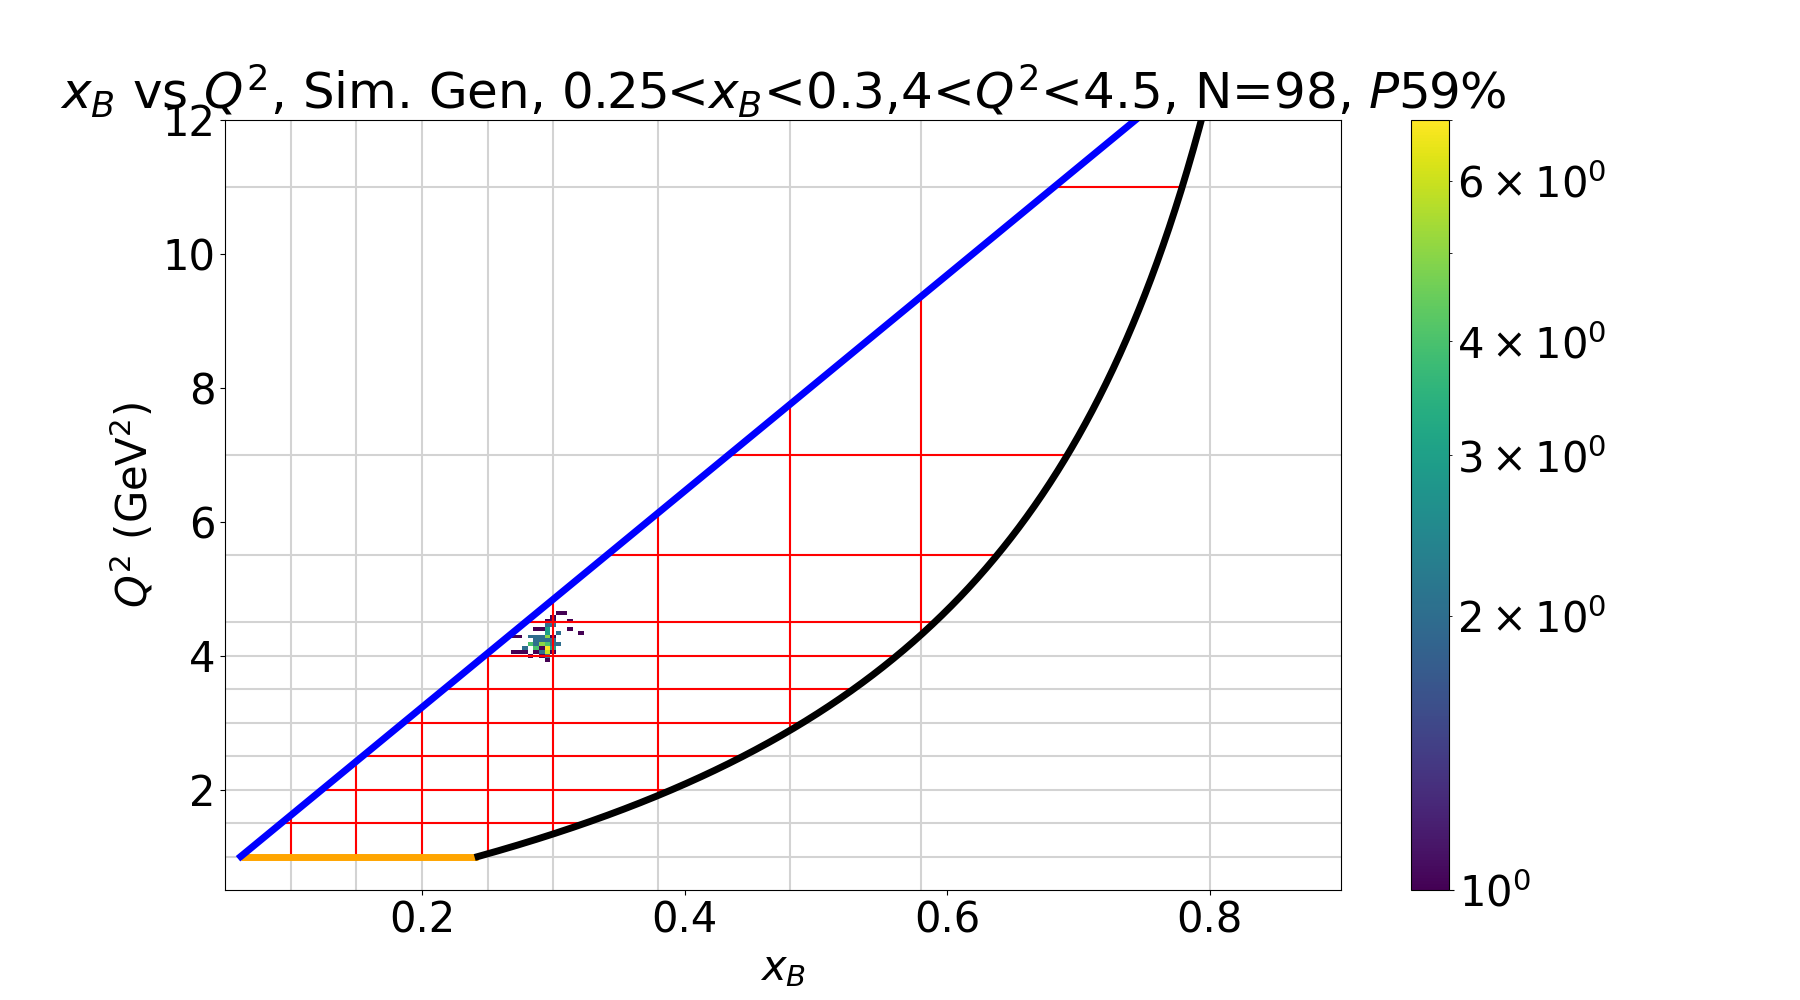
\includegraphics[trim={0 0 10cm 3.5cm},clip,width=0.5\textwidth]{Chapters/Ch5-Further/0_IBU/pics/migration_example/x_B_vs_Q2,_Sim_Gen,_025x_B03,4Q245,_N=98,_P59.png}
        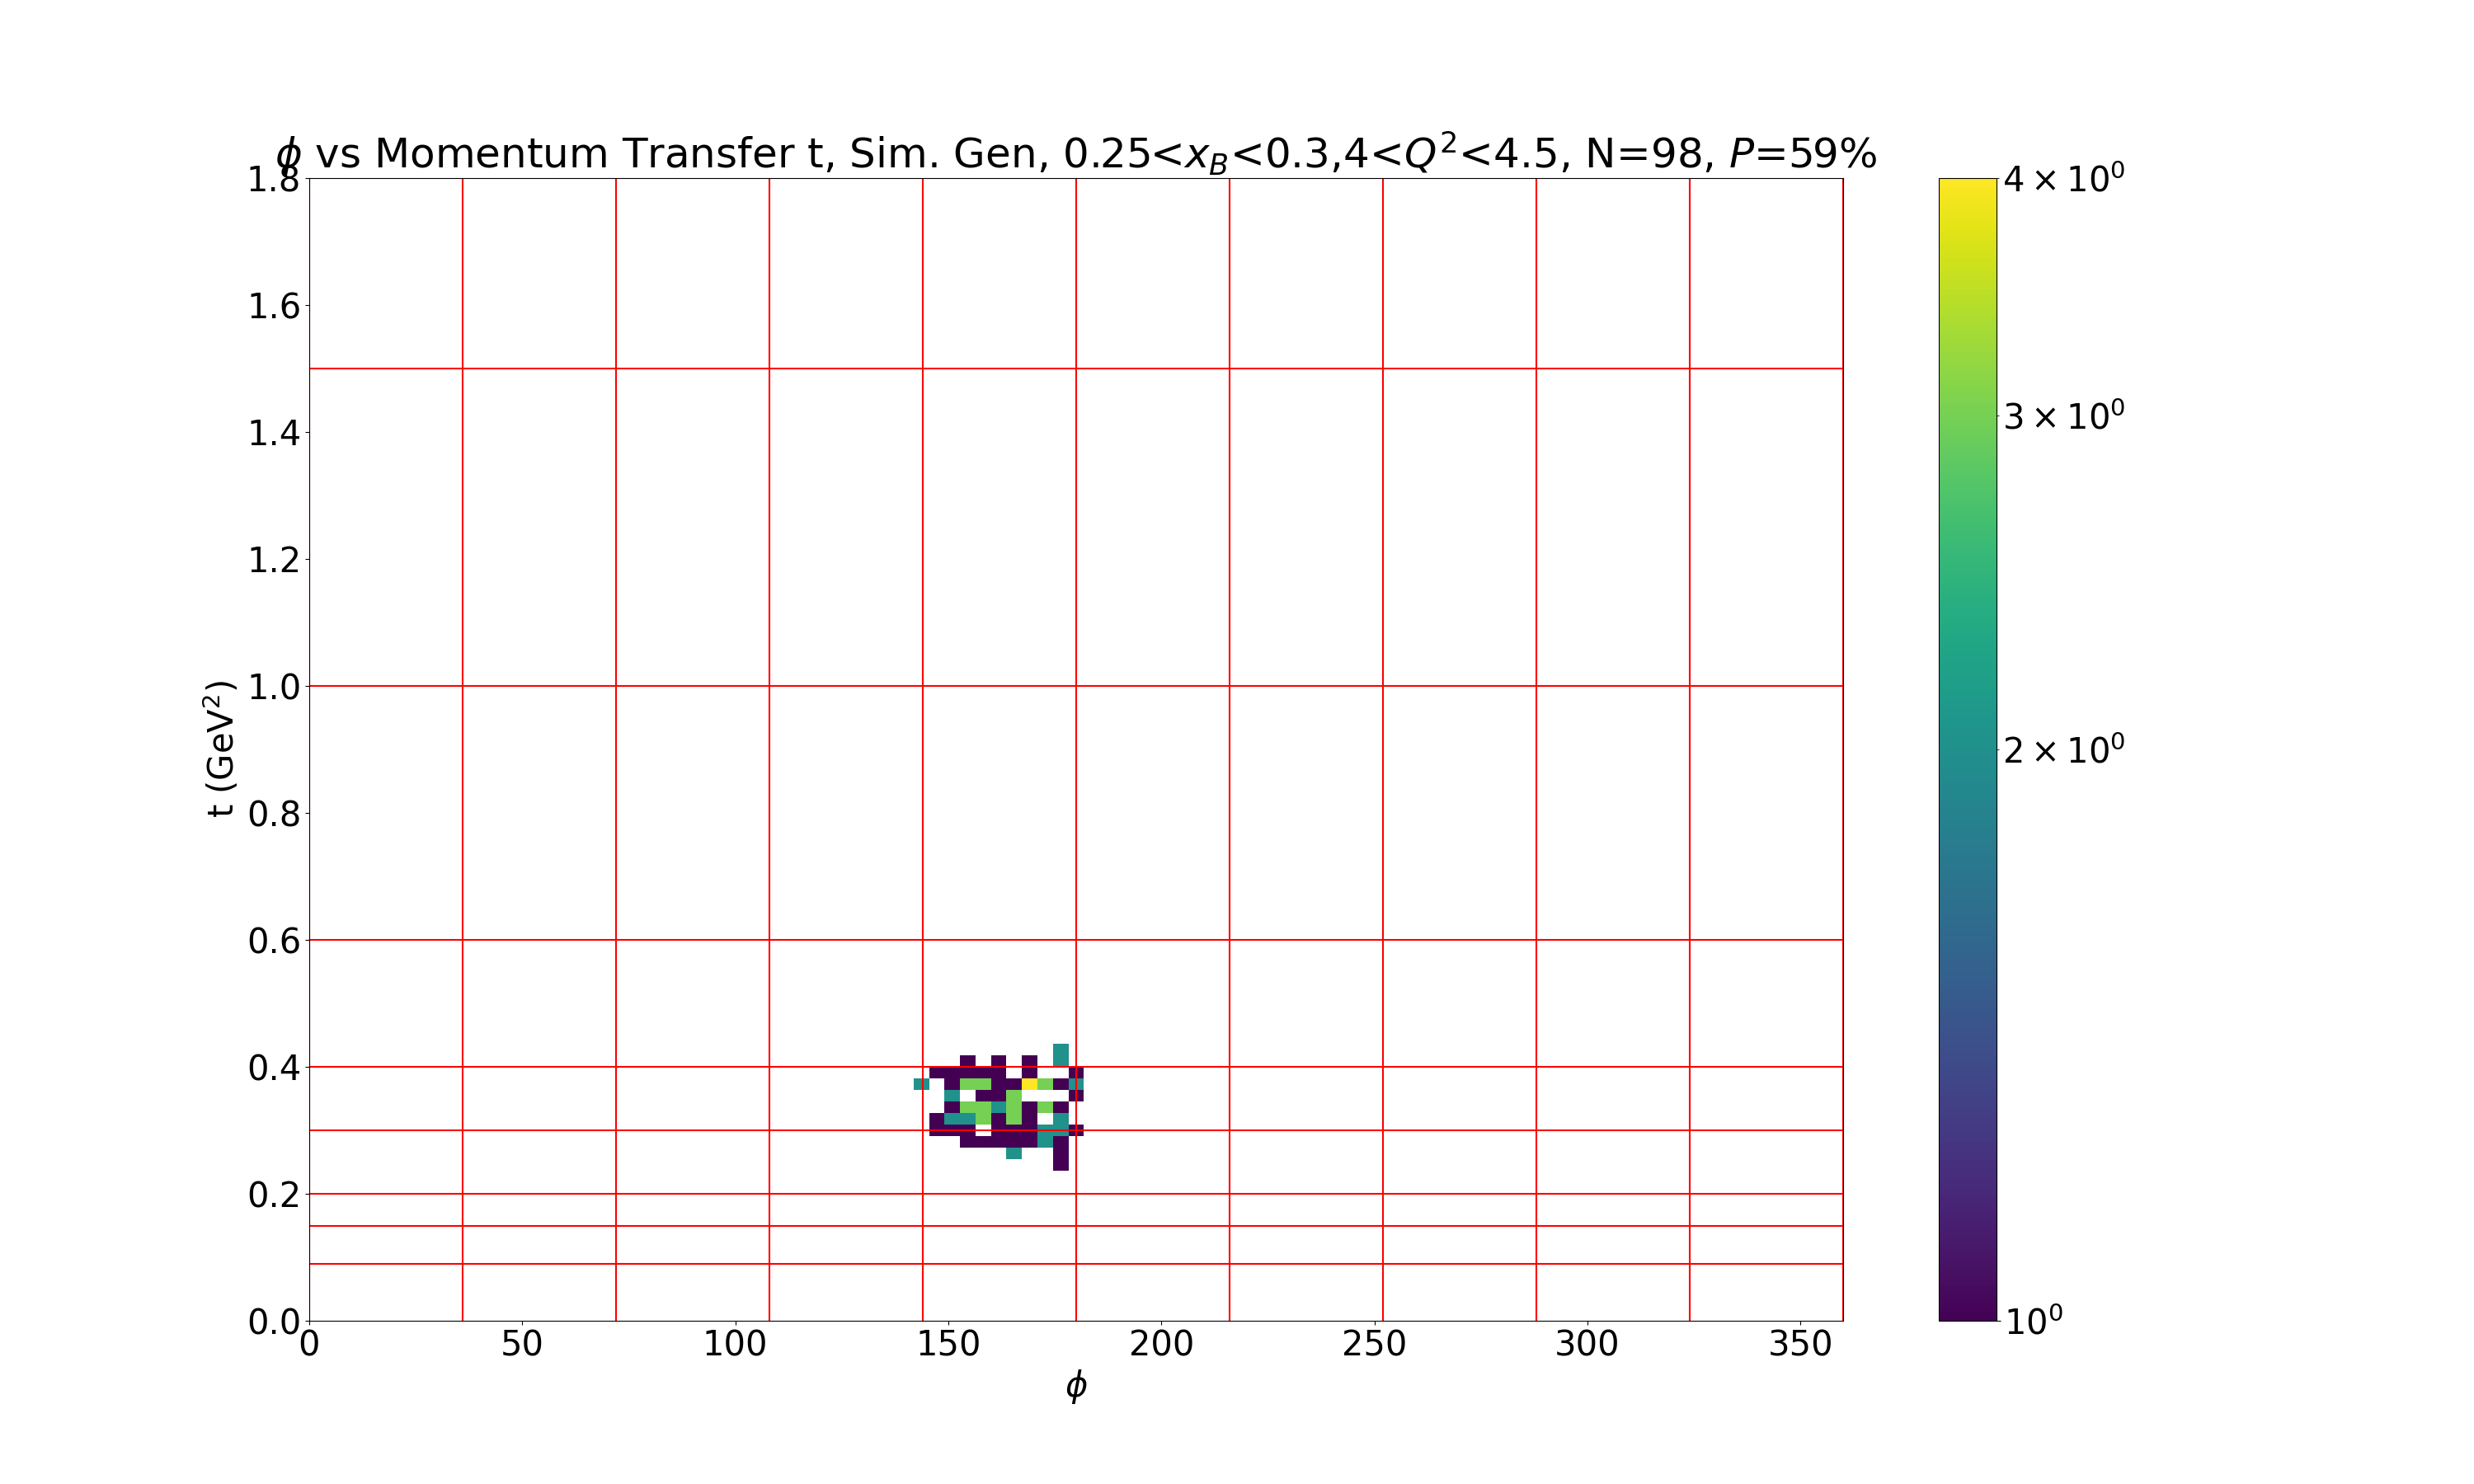
\includegraphics[trim={0 0 17.5cm 6cm},clip,width=0.45\textwidth]{Chapters/Ch5-Further/0_IBU/pics/migration_example/phi_vs_Momentum_Transfer_t,_Sim_Gen,_025x_B03,4Q245,_N=98,_P=59.png}
        \label{fig:generated_events}
    }

    \caption[Bin Migration Example]{Binning migration example in a particular 4-D bin. Note that all events reside within a single bin for the reconstructed dataset (top), but not all events that were observed in that bin was generated in that same bin (bottom).}\label{fig:mig_example}
\end{figure}

Bin migrations can be described by two quantities: bin purity $P_{i}$ \eqref{eq:bin_purity}, which describes the fraction of events observed in bin i $N_{obs,i}$ that truly belong, or were generated, in that bin $N_{truth,i}$, 

    \begin{equation}
    P_{i} = \frac{N_{obs,i}}{N_{gen,i}},
    \end{equation}\label{eq:bin_purity}
    \myequations{ Bin Purity}

    and bin efficiency  $E_{i}$ \eqref{eq:bin_efficiency}, which is the fraction of the number of events that were generated in bin i $N_{truth,i}$ that were also observed in bin i, $N_{obs,i}$ 

    \begin{equation}\label{eq:bin_efficiency}
    E_{i} = \frac{N_{gen\&obs,i}}{N_{gen,i}}.
    \end{equation}
    \myequations{Bin Efficiency}

Multi-dimensional datasets are particularly susceptible to bin migration issues: an analysis that has 80\% bin purity in each of four dimensions yields a 4D bin that has a purity of only 0.8$^4$=41\%. \figref{fig:bin_purity_tphi} shows the bin purities for example $x_B-Q^2$ bins across t and $\phi$ which are relatively high and low for the dataset. 
    

        \iffalse
    t1 mean purity:  0.5779366649713987
    t1 mean efficiency:  0.6042514773951323
    t2 mean purity:  0.7249045469386235
    t2 mean efficiency:  0.7344406993707698
    t1 rad mean purity:  0.5959652676783339
    t1 rad mean efficiency:  0.6213147478696212
    t2 rad mean purity:  0.7423936456812074
    t2 rad mean efficiency:  0.7511469995793438
    \fi 

        
\begin{figure}[H]
    \centering
    \subfloat[Bin purities for an example set of t-$\phi$ bins for a single $x_B$-$Q^2$ bin with high bin purity.]{%
        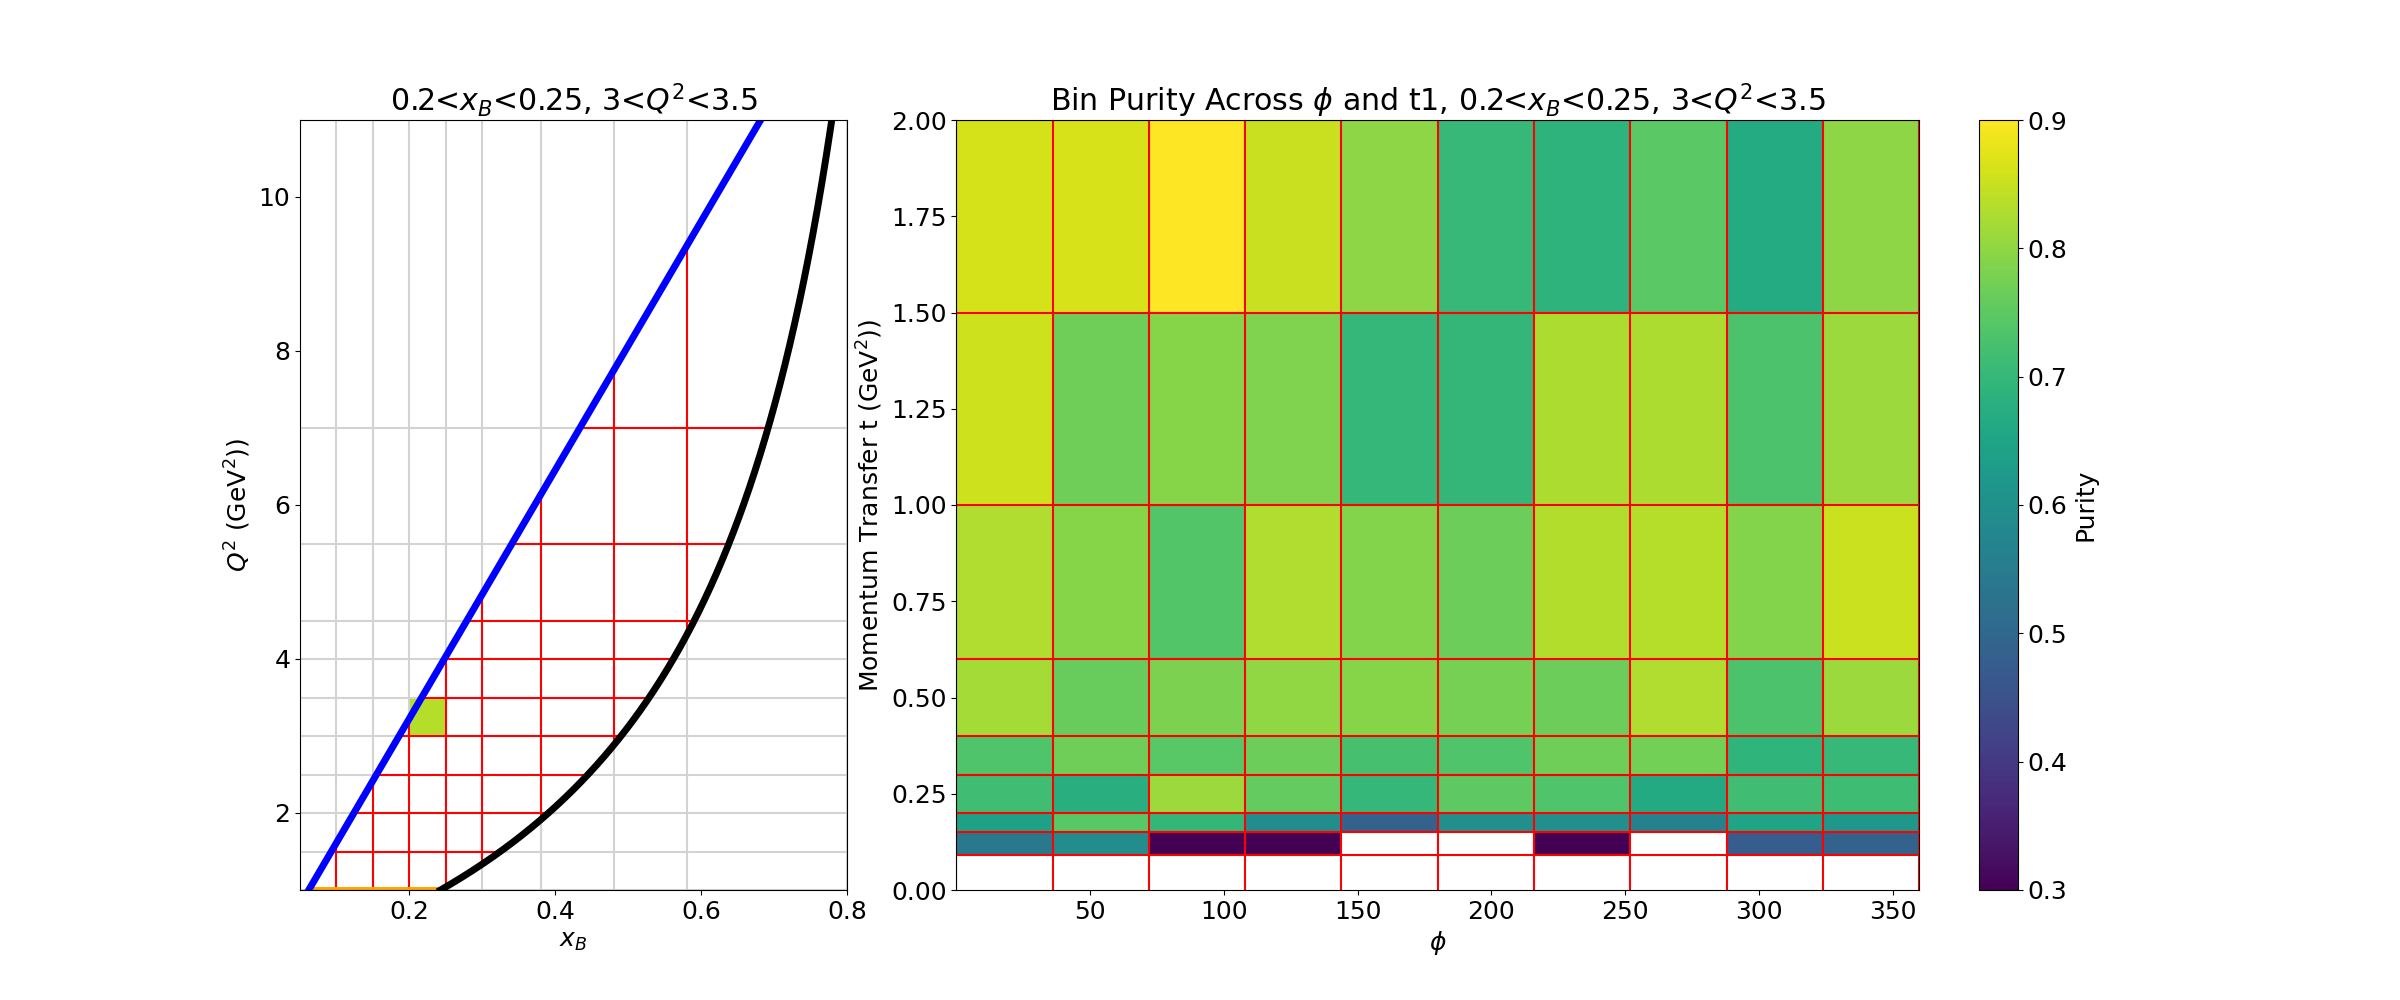
\includegraphics[trim={0 0 0 0},clip,width=.8\textwidth]{Chapters/Ch5-Further/0_IBU/pics/complete/testfig.png}
        \label{fig:ex1_binP}
    }\\
    \subfloat[Bin purities for an example set of t-$\phi$ bins for a single $x_B$-$Q^2$ bin with low bin purity.]{%
        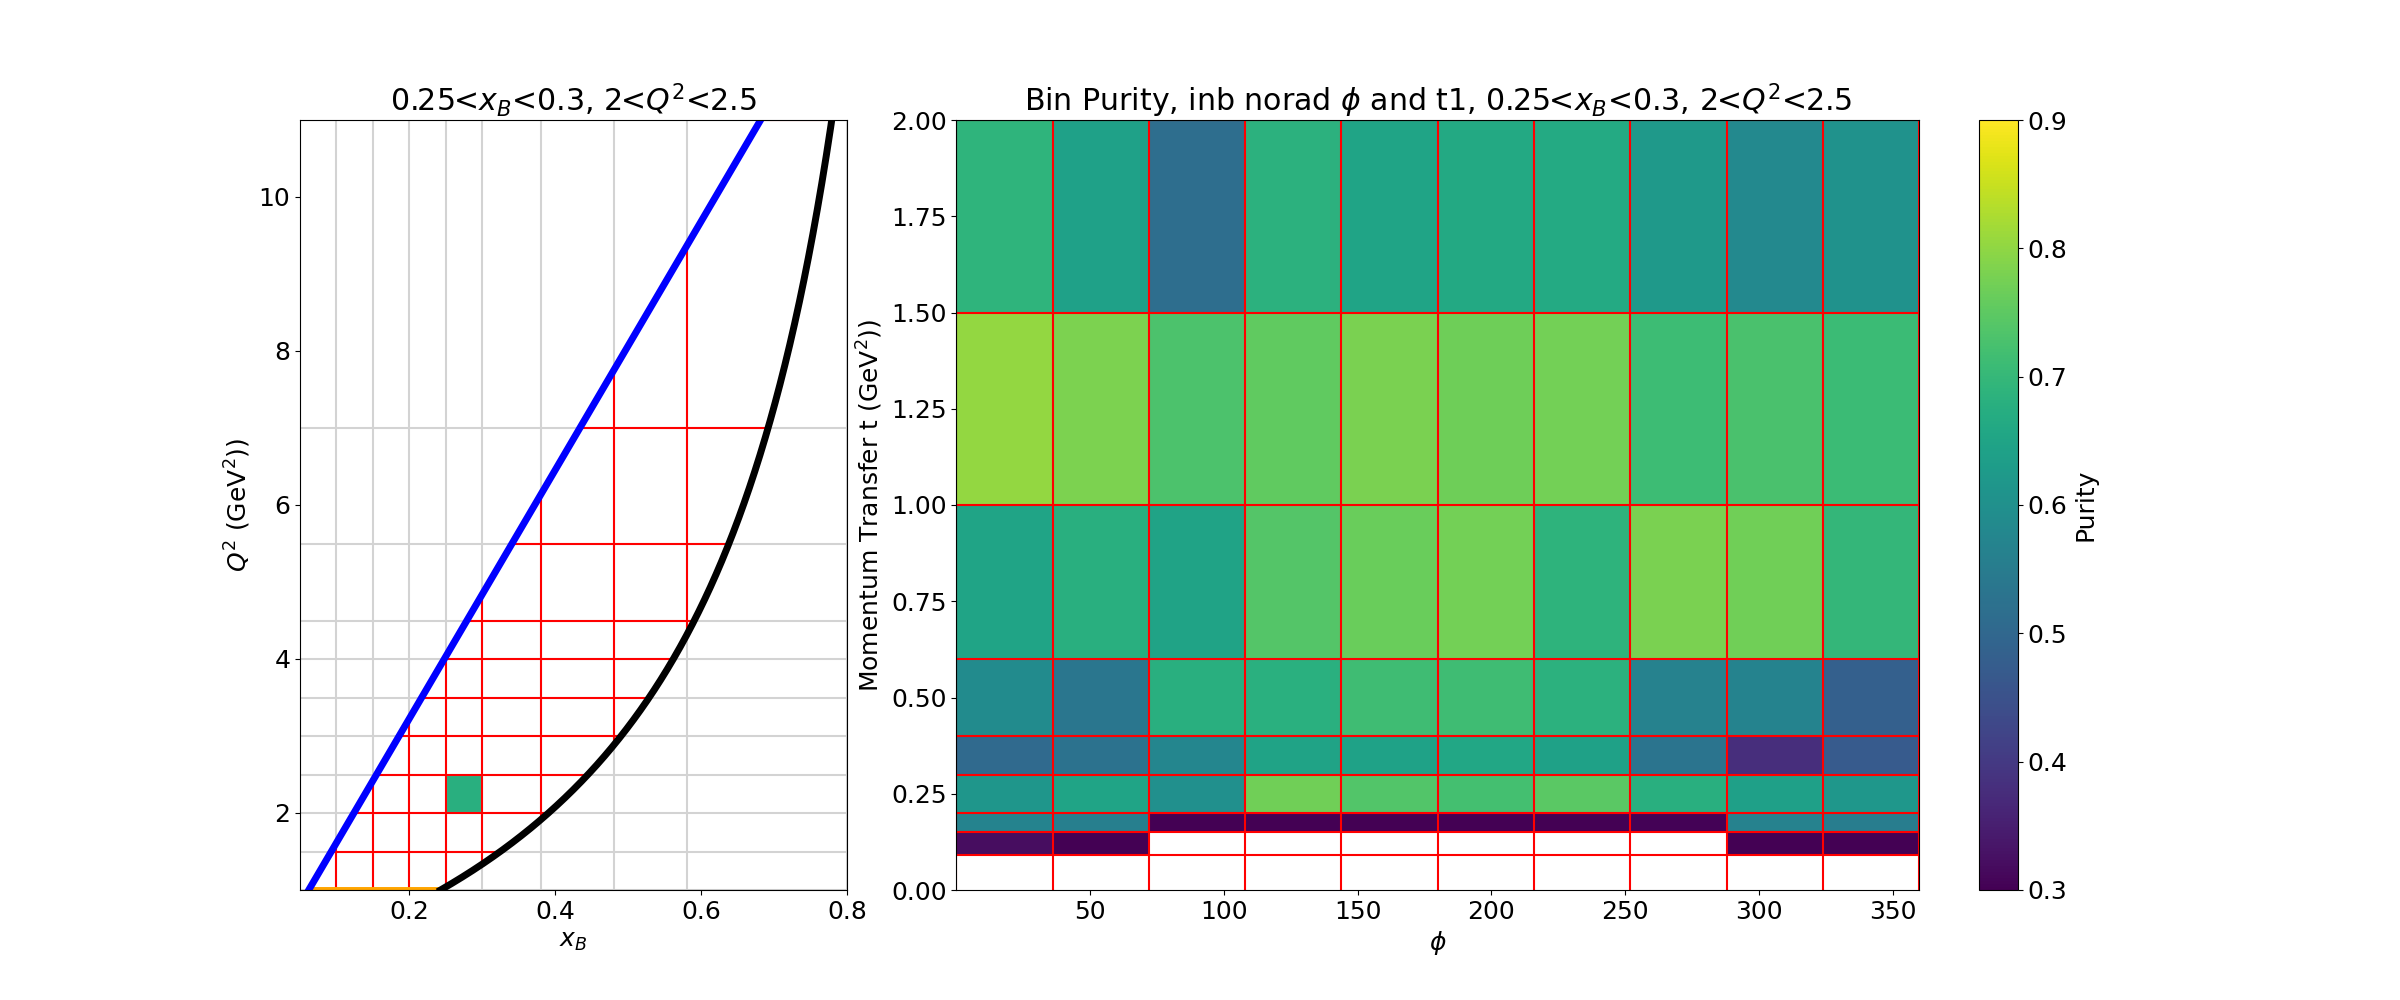
\includegraphics[trim={0 0 0 0},clip,width=.8\textwidth]{Chapters/Ch5-Further/0_IBU/pics/purities/inb_norad_t1/bin_purity_0.25_0.3_2_2.5.png}
        \label{fig:ibu10}
    }
    \caption[Bin Purity Example Distributions]{Example bins with relatively high (a) and low (b) bin purities.}\label{fig:bin_purity_tphi}
\end{figure}


    The distribution of purities and efficiencies for all bins can be seen in in \figref{fig:bin_purity_eff_hist}. With present analysis algorithms, we observe a mean bin purity of 58\% and mean bin efficiency is 60\%.

    \begin{figure}[H]
        \centering
        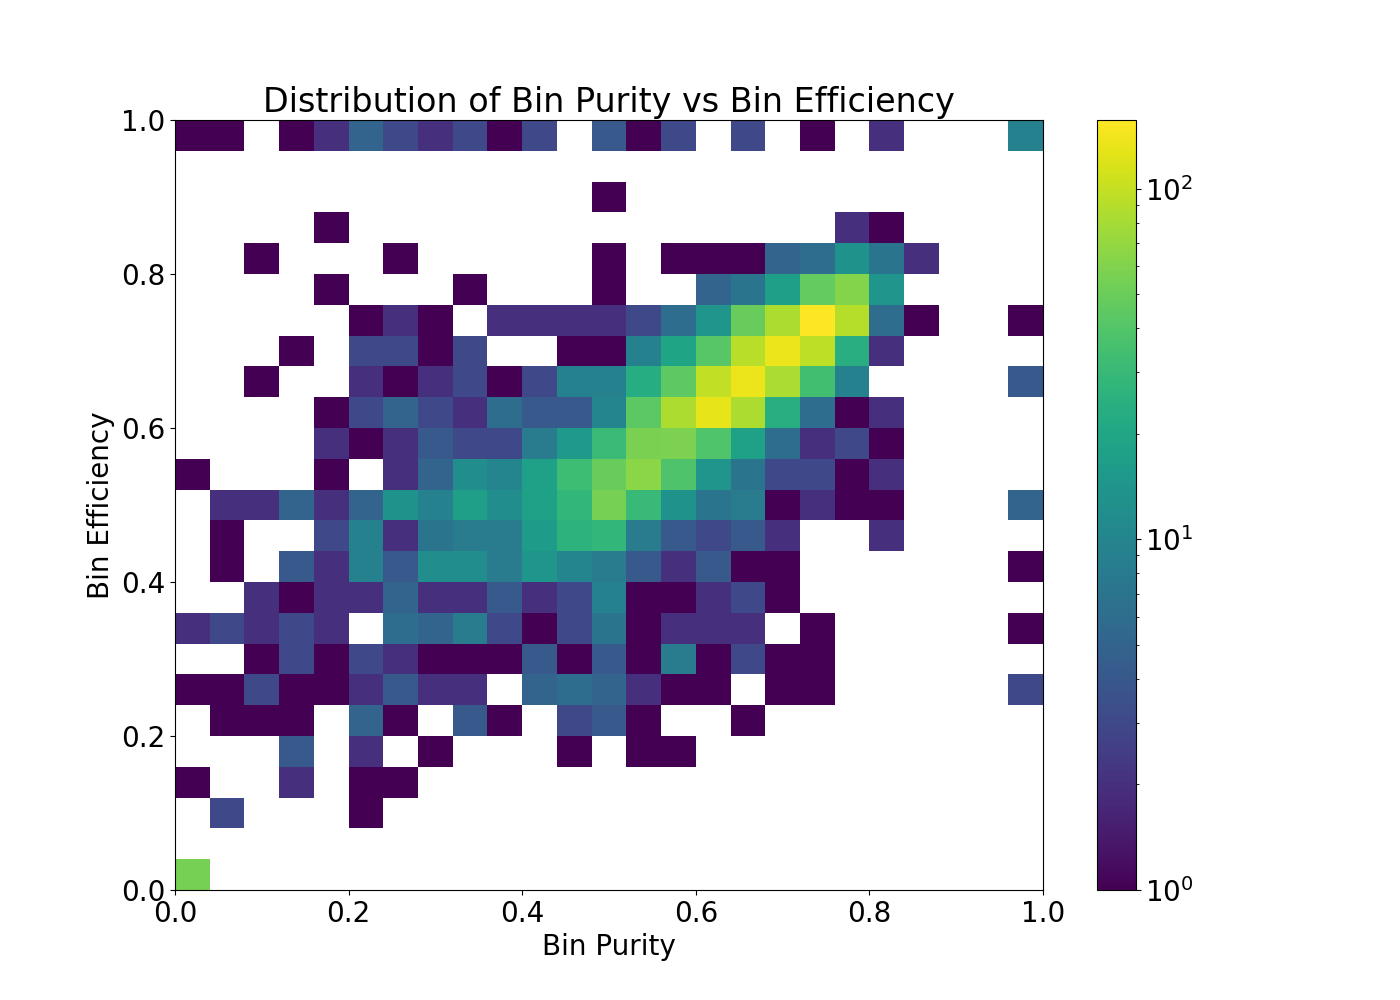
\includegraphics[trim={0 0 0 0},clip,width=0.8\textwidth]{Chapters/Ch5-Further/0_IBU/pics/overview/t1_bin_purity_vs_bin_efficiency.png}
        \caption[Bin Purity - Efficiency Distribution]{Distribution of bin purities and efficiencies for the Fall 2018 inbending configuration, determined from simulations.}
        \label{fig:bin_purity_eff_hist}
    \end{figure}


    Bin migrations are unavoidable, especially in four dimensions. No systematic offsets are known, but the resolution on the \textit{t} binning variable is relatively low compared to the other three, as displayed in \figref{fig:binning_resolutions} which compares the difference in generated and reconstructed variables as a function of that variable. 
    
    \begin{figure}[H]
        \centering
        \subfloat[][$x_B$.]{
        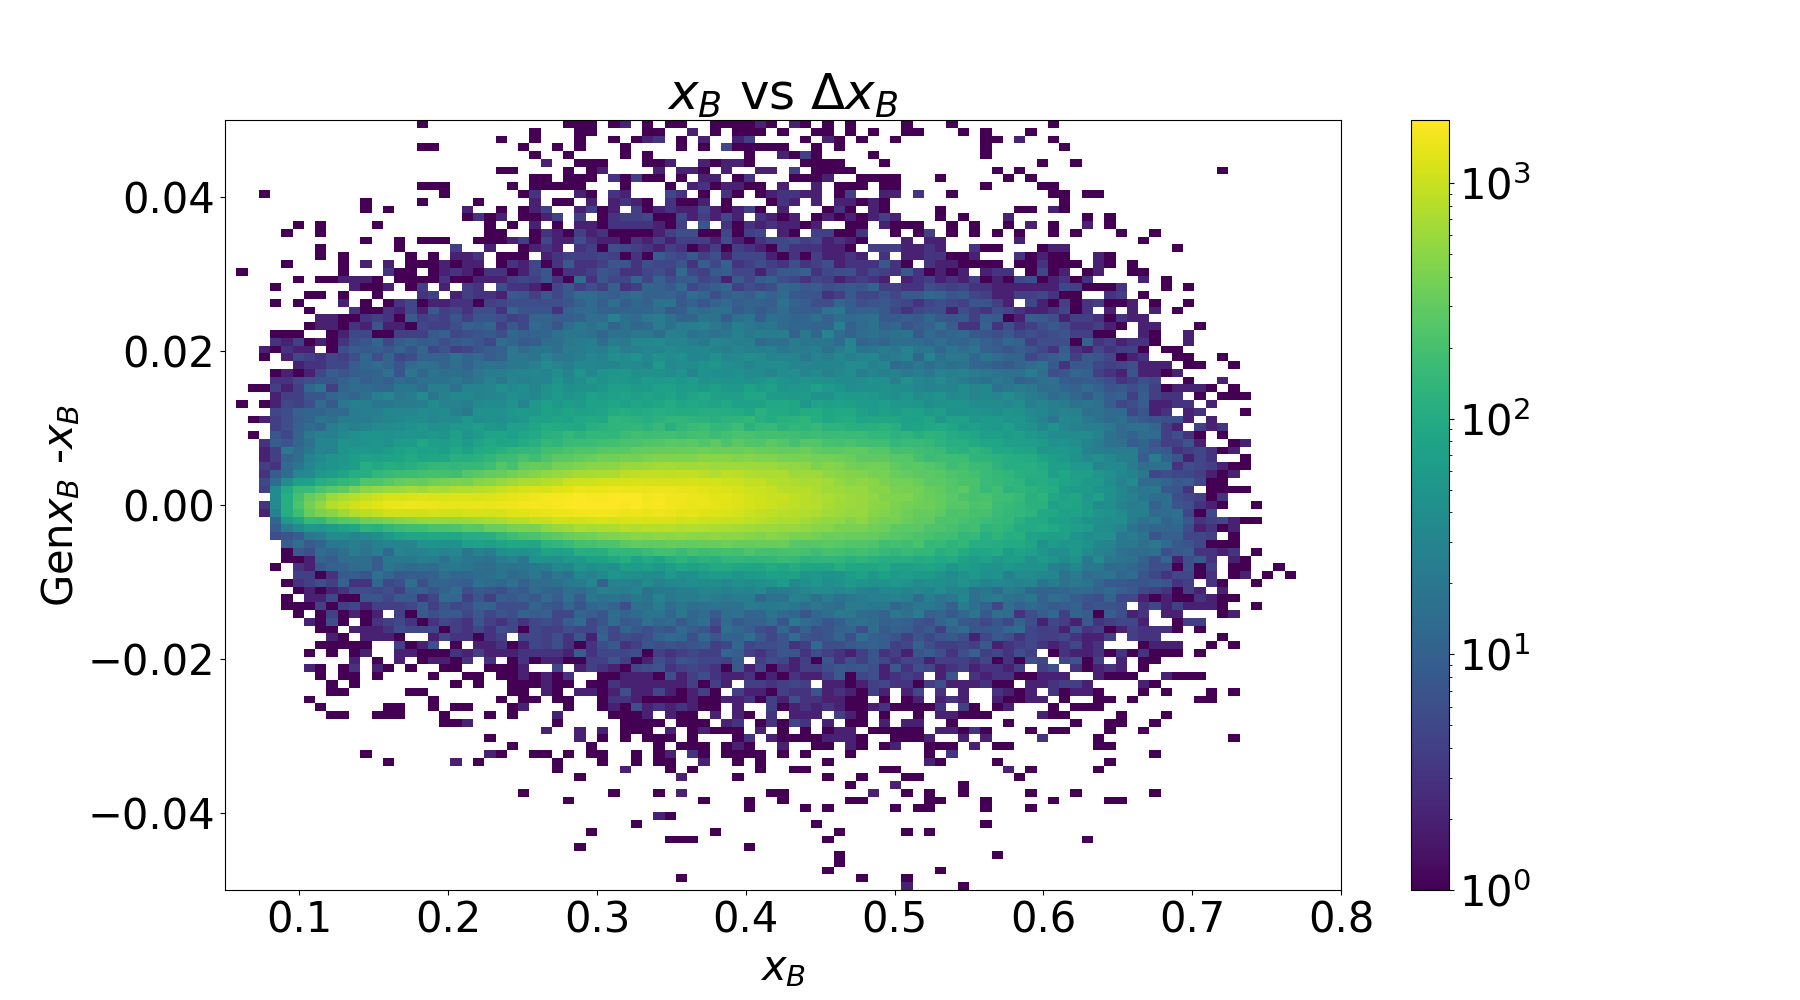
\includegraphics[width=0.4485\textwidth]{Chapters/Ch5-Further/0_IBU/pics/migrations/x_B_vs_Delta_x_B.png}
        \label{fig:binning_resolutionsa}}
        \hfill
        \subfloat[][$Q^2$.]{
        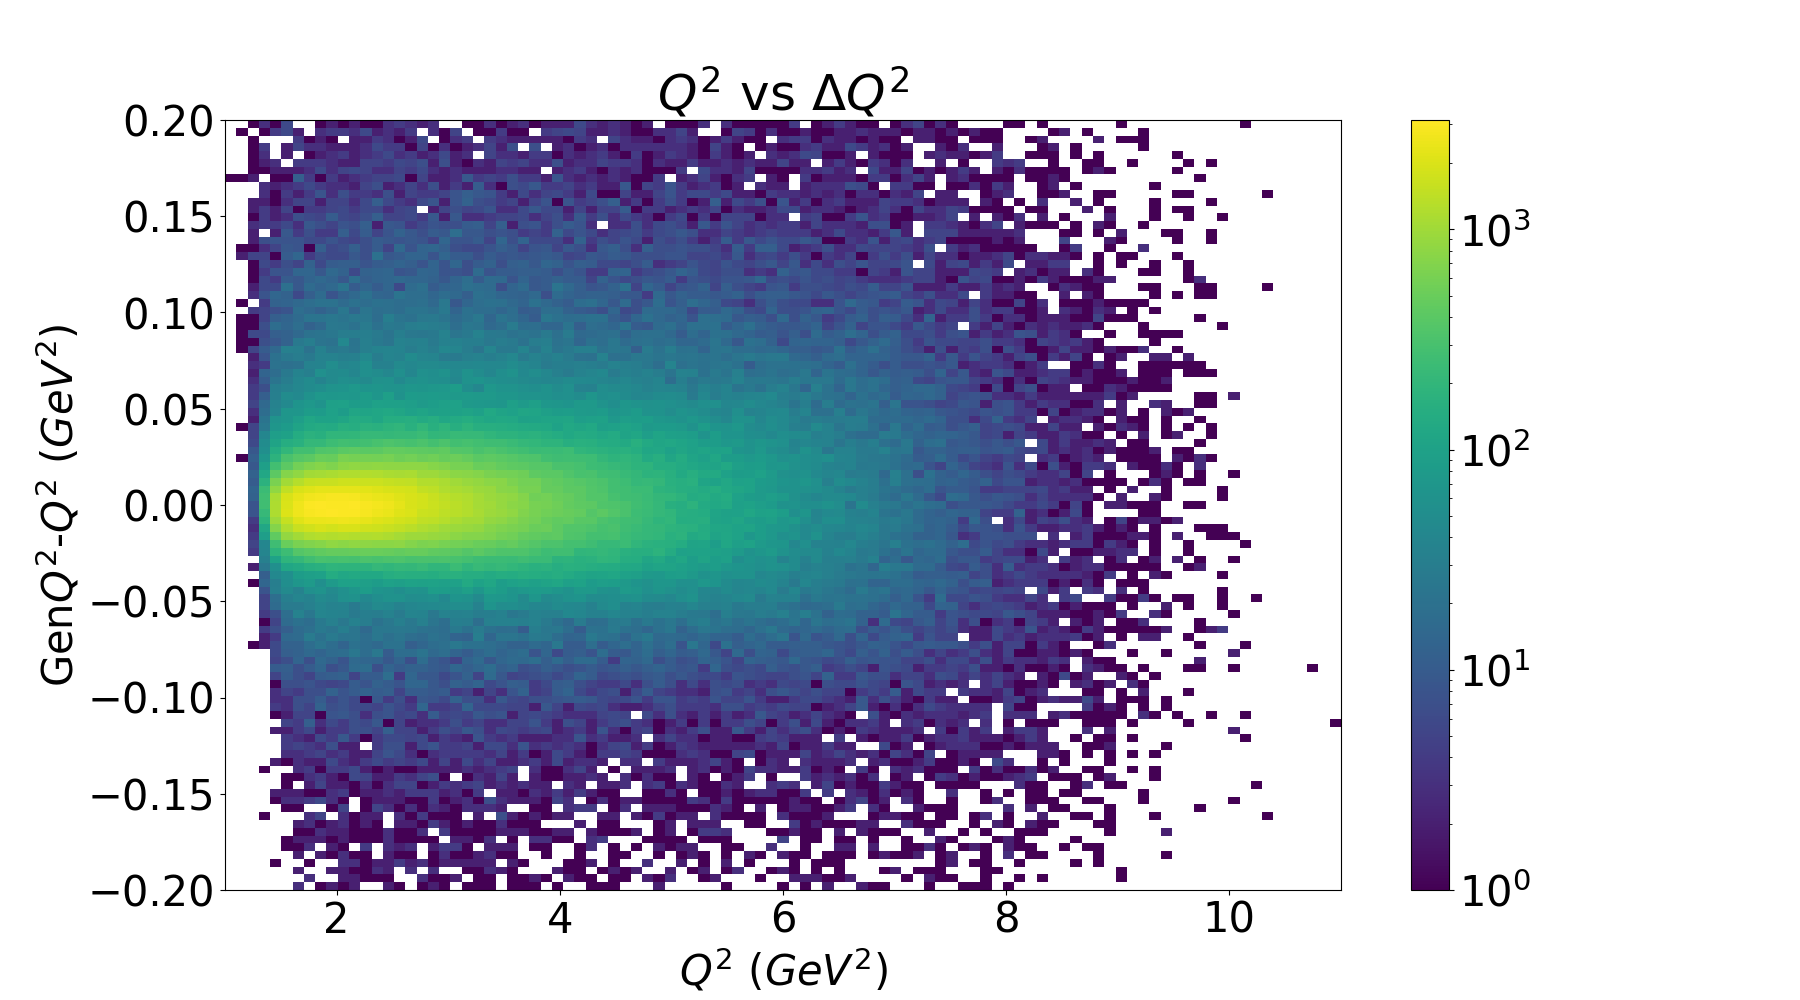
\includegraphics[width=0.4485\textwidth]{Chapters/Ch5-Further/0_IBU/pics/migrations/Q2_vs_Delta_Q2.png}
        \label{fig:binning_resolutionsb}}
        \\
        \subfloat[][$\phi$.]{
        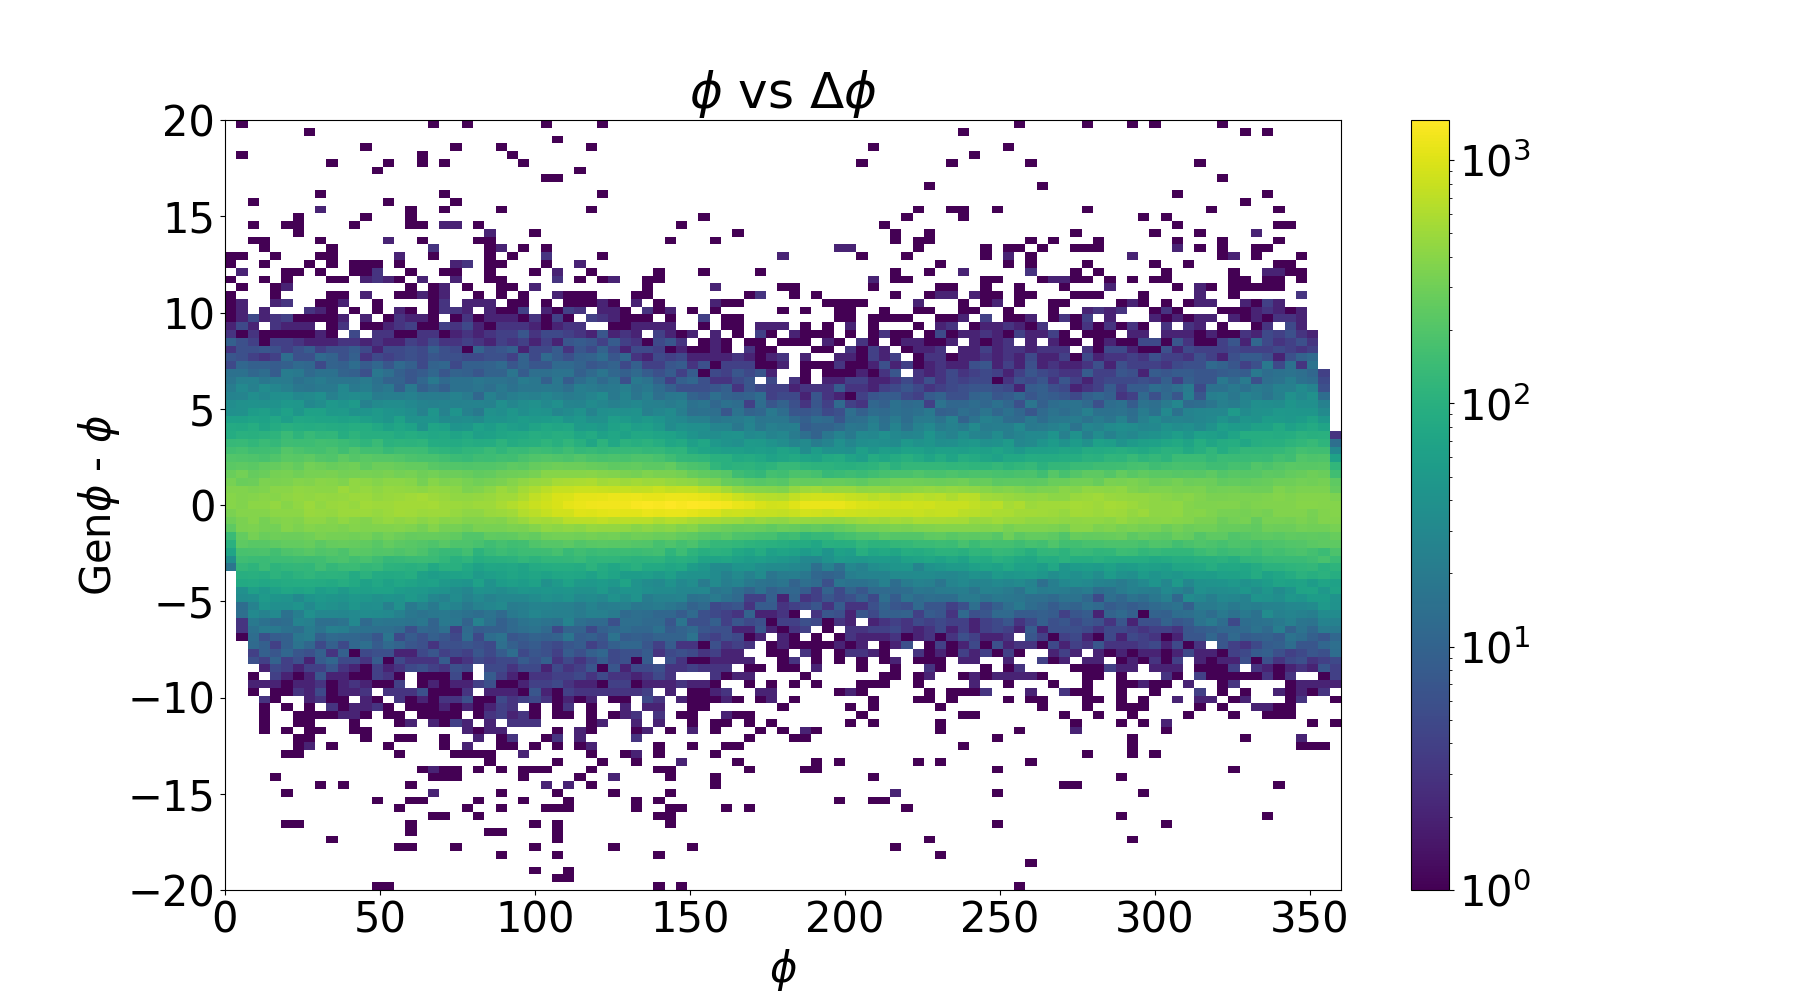
\includegraphics[width=0.4485\textwidth]{Chapters/Ch5-Further/0_IBU/pics/migrations/phi_vs_Delta_phi.png}
        \label{fig:binning_resolutionsc}}
        \hfill
        \subfloat[][t.]{
        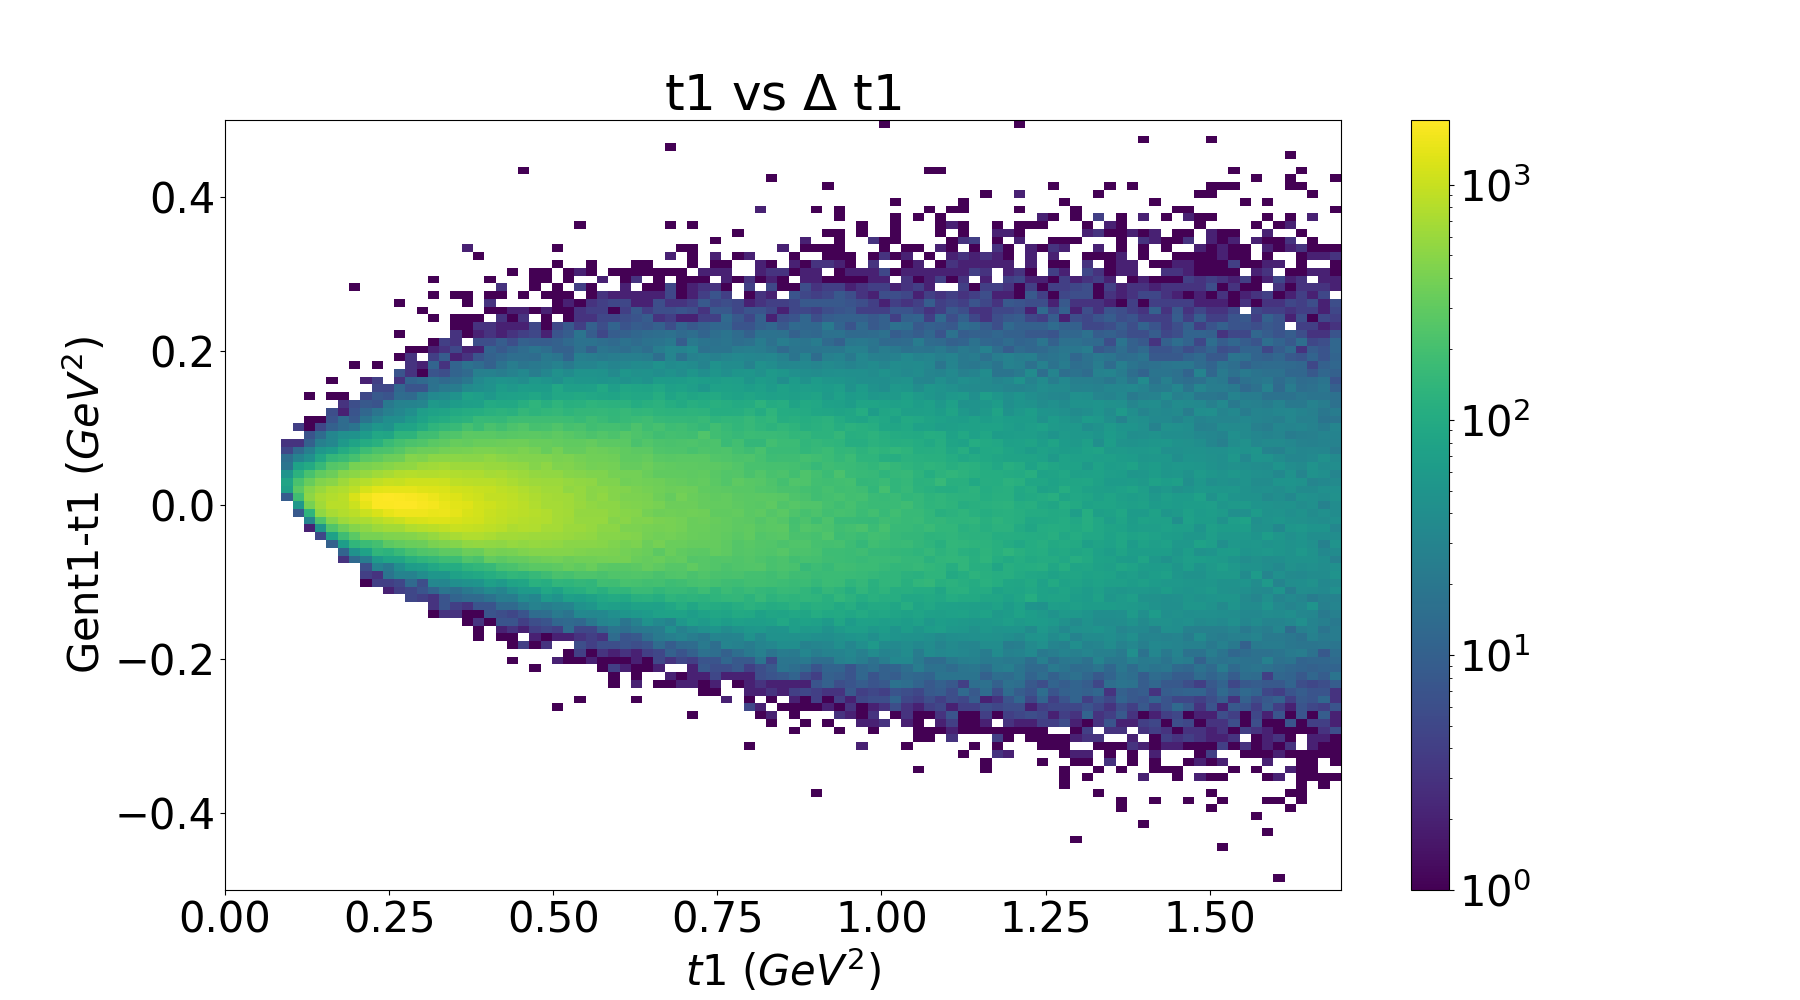
\includegraphics[width=0.4485\textwidth]{Chapters/Ch5-Further/0_IBU/pics/migrations/t1_vs_Delta_t1.png}
        \label{fig:binning_resolutionsd}}
        \caption[Binning Variable Resolutions]{Reconstruction resolution for $x_B$ (a), $Q^2$ (b), $\phi$ (c) and t (d).}
        \label{fig:binning_resolutions}
    \end{figure}
    
    By superimposing a periodic waving to illustrate point locality \figref{fig:bin_waving}, we can observe drifts between generated and reconstructed positions. Improvements to base code are currently being developed as part of a collaboration-wide effort to increase reconstruction resolution performance. In principle, unfolding methods will always be a necessary component of a full analysis, but are particularly significant when bin purities are low. 
    
    \begin{figure}[H]
        \centering
        \subfloat[][$x_B$ true (left) vs. observed locations.]{
        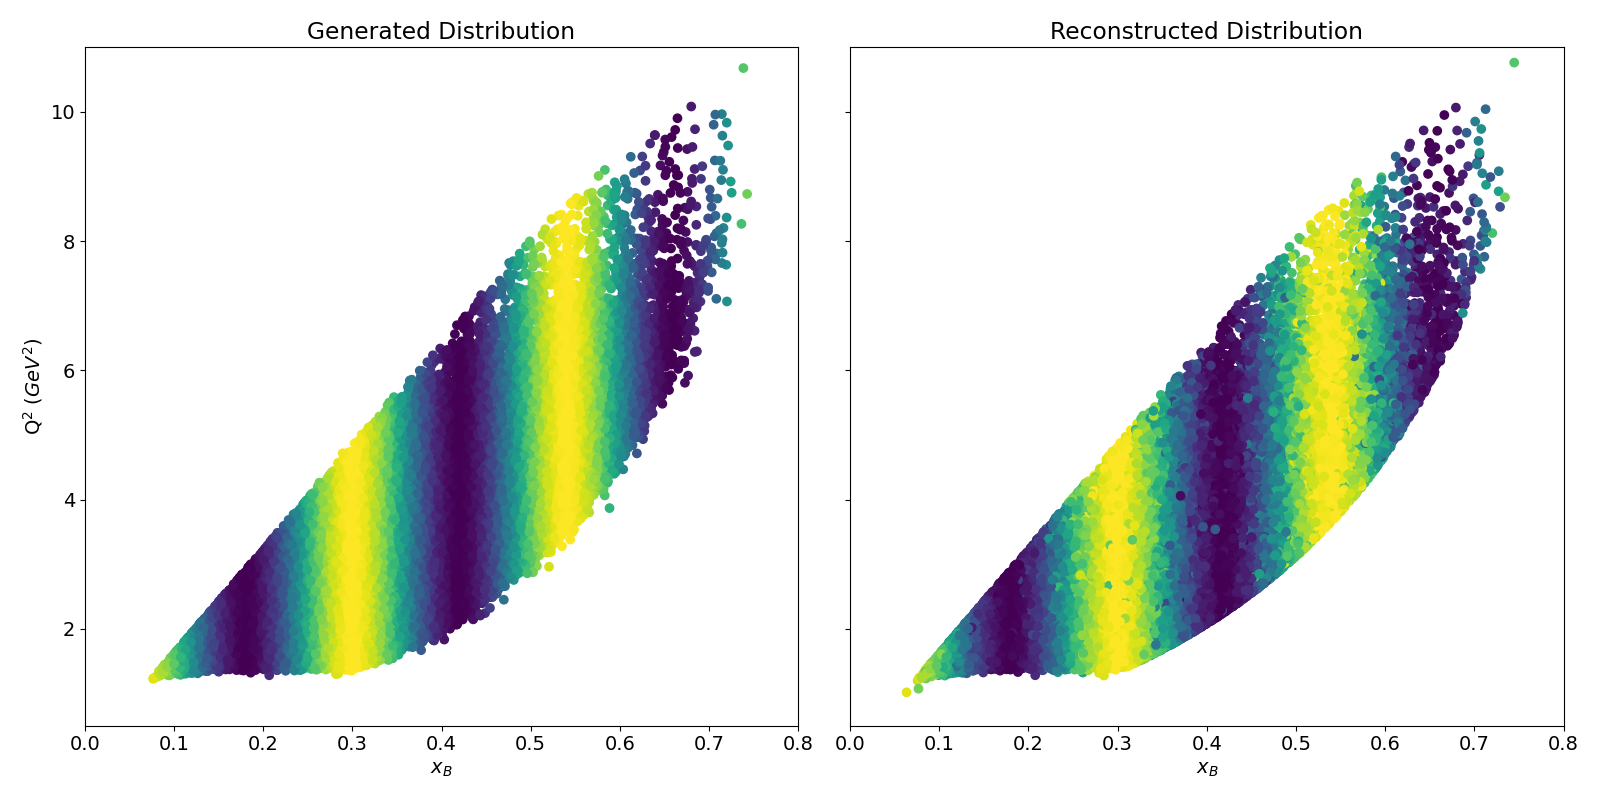
\includegraphics[width=0.45\textwidth]{Chapters/Ch5-Further/0_IBU/pics/waving/sine_plots_xB.png}
        \label{fig:ibu4a}}
        \hfill
        \subfloat[][$Q^2$ true (left) vs. observed locations.]{
        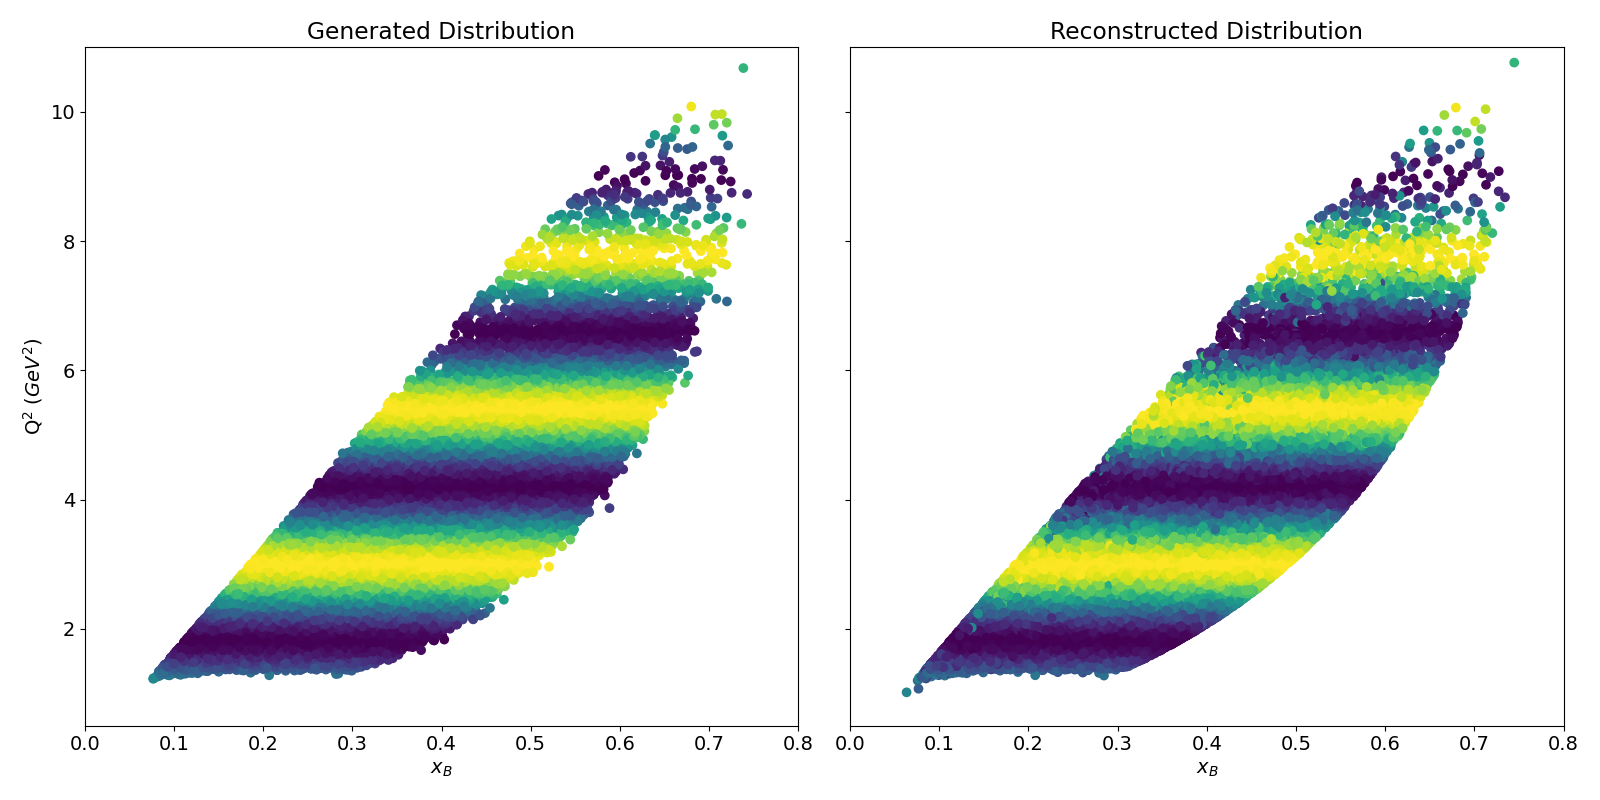
\includegraphics[width=0.45\textwidth]{Chapters/Ch5-Further/0_IBU/pics/waving/sine_plots_Q2.png}
        \label{fig:ibu4b}}
        \\
        \subfloat[][$\phi$ true (left) vs. observed locations.]{
        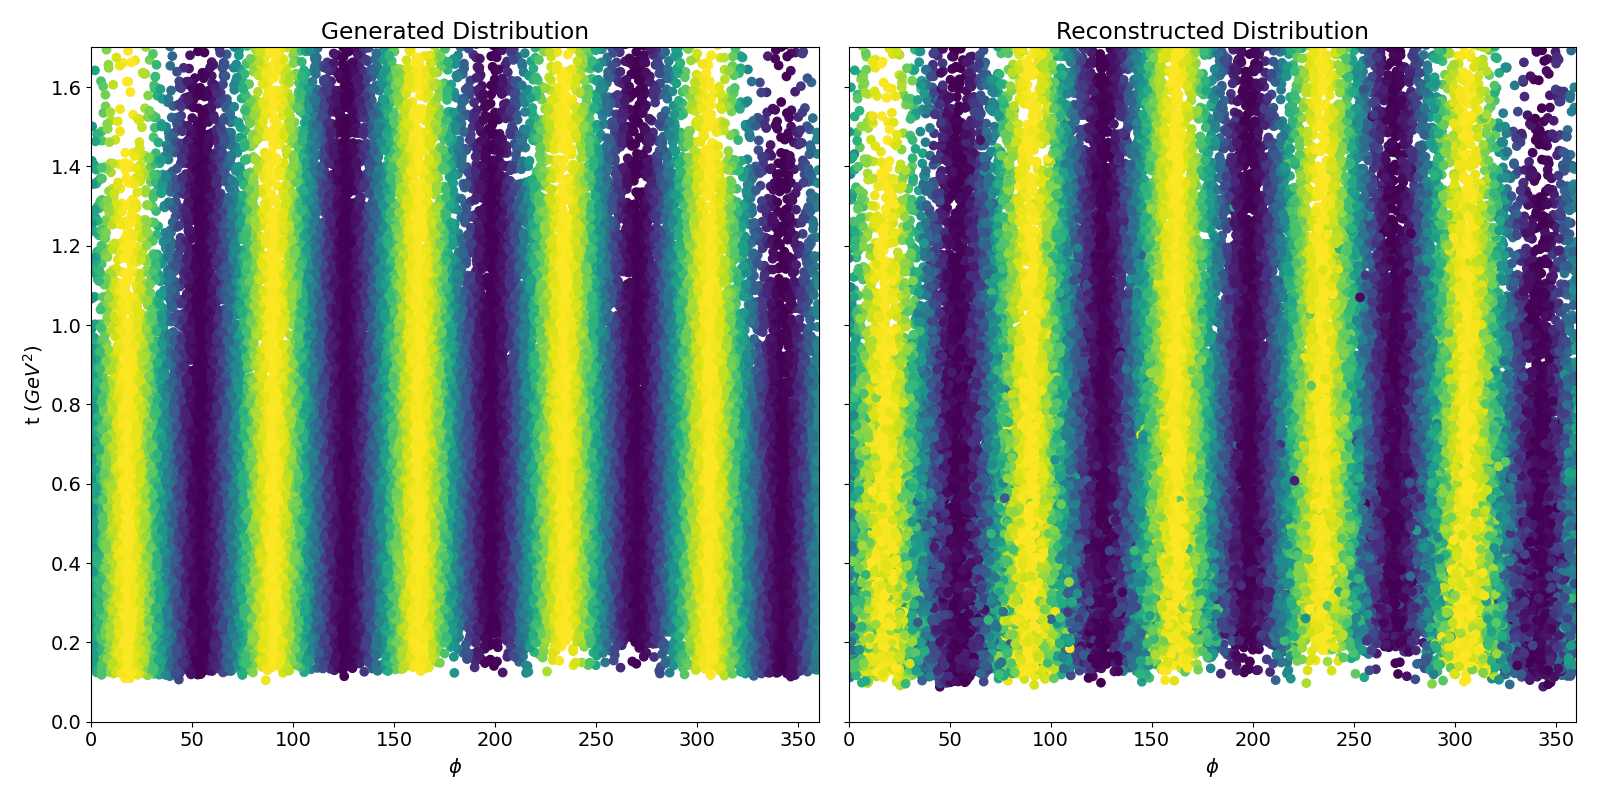
\includegraphics[width=0.45\textwidth]{Chapters/Ch5-Further/0_IBU/pics/waving/sine_plots_phi.png}
        \label{fig:ibu4c}}
        \hfill
        \subfloat[][t true (left) vs. observed locations.]{
        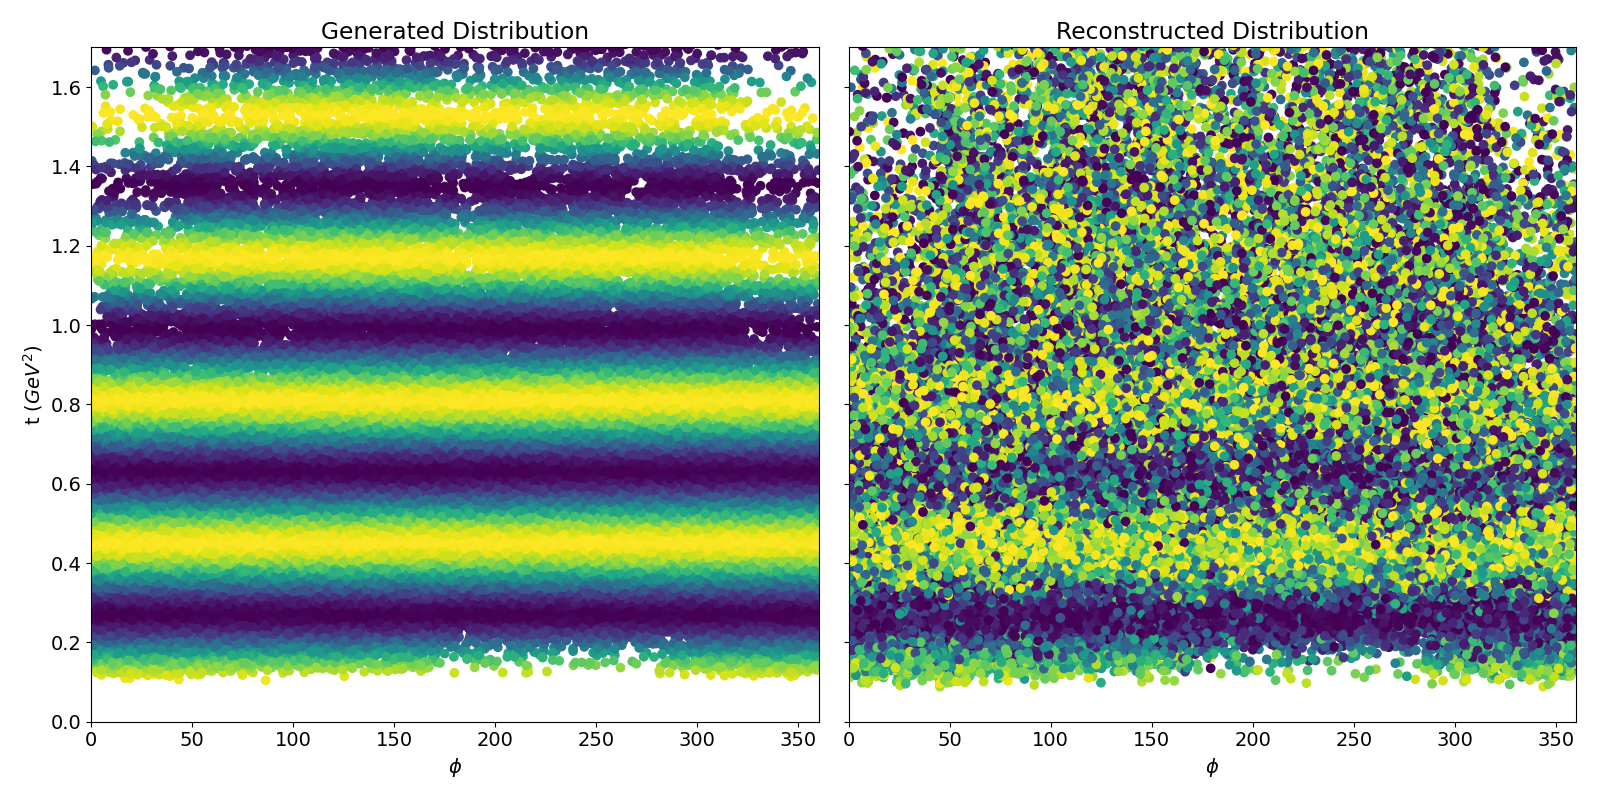
\includegraphics[width=0.45\textwidth]{Chapters/Ch5-Further/0_IBU/pics/waving/sine_plots_t.png}
        \label{fig:ibu4d}}
        \caption[Truth vs. Observed Binning Variable Samples]{Pattern matching illustrations for $x_B$ (a), $Q^2$ (b), $\phi$ (c) and t (d). For all variables, sample events were color coded based off the sine of the respective variable generated value. Discrepancies between patterns are indicative of reconstruction resolution. Note that this visualization technique can not illustrate shifts of the same frequency of the overlaid sine wave.}
        \label{fig:bin_waving}
    \end{figure}
    %Could index off of t2 missing mass, but not ideal for radiative corrections and in general want 
    

    Full information can be encapsulated in a \textbf{response matrix}, which for n bins is an nxn matrix with element $R_{i,j}$ describing the number of events generated in bin i and observed in bin j. A response matrix for a perfect system would be the identity matrix. This matrix is often normalized, such that its elements describe the probability of an event that is generated in bin i being observed in bin j. This matrix can be leveraged by a number of unfolding techniques to untangle bin migration effects and obtain a better understanding of the true distribution of the system. 


 \clearpage

\section{Iterative Bayesian Unfolding}

    \subsection{Data Unfolding}

        Unfolding is a general term used to describe procedures focused on estimating the true underlying distribution of a system from measured data which has imperfections due to for example detector responses or reconstruction algorithm and modeling limits. Methods include Singular Value Decomposition \parencite{Klema1980TheApplications}, Fully Bayesian Unfolding \cite{Choudalakis2012FullyUnfolding}, or Tikhonov regularization \parencite{Hoerl1970RidgeProblems}. Each method comes with benefits and pitfalls; this analysis utilizes Iterative Bayesian Unfolding (IBU) \parencite{DAgostini1995ATheorem}, \parencite{DAgostini2010ImprovedUnfolding} for its ability to handle multidimensional unfolding and complicated detector and reconstruction response functions, as well as its facile tracking of systematic and statistical uncertainties. 

        Unfolding methods aim to determine the inverse of a response matrix \textbf{R}, where a true underlying distribution \textbf{x} and a corresponding observed distribution \textbf{y} are related by \textbf{y}=\textbf{Rx}. In general \textbf{R} may be poorly conditioned, non-smooth, and otherwise not amenable to direct inversion. IBU approaches this problem by beginning with Bayes' Theorem \eqref{eq:bayes},

        \begin{equation}\label{eq:bayes}
            P(A|B) = \frac{P(B|A) \cdot P(A)}{P(B)},
        \end{equation}
        \myequations{Bayes' Theorem}

        which relates the conditional probability of observing event A given B to the conditional probability of observing B given A. In particular, if event A represents observing an event x in bin i, and B represents event x truly belonging to bin j, then we can rewrite Bayes' theorem as \eqref{eq:bayes_reform}


        \begin{equation}\label{eq:bayes_reform}
            R_{ij} = P(x \in \text{bin } i| x \in \text{bin } j) = \frac{P(x \in \text{bin } j|x \in \text{bin } i) \cdot P(x \in \text{bin } i)}{P(x \in \text{bin } j)},
        \end{equation}
        \myequations{Bayes' Theorem}


        where $R_{ij}$ are just the elements of the response matrix. Then, inverting Bayes' Theorem allows for calculating the individual matrix elements of the unfolding function, which can be approached iteratively from some initial starting guess (prior). 

        In particular, IBU begins with an initial estimate of the true distribution, and in each iteration, it modifies this estimate based on the residuals between the measured data and the data predicted by the current estimate. The iterations continue until the estimate converges to a stable solution, defined by a hyperparameter stopping criterion. 
        %P(C_i | E_j, I) = \frac{P(E_j | C_i, I) \cdot P(C_i | I)}{\sum_i P(E_j | C_i, I) \cdot P(C_i | I)}


        
        \iffalse
        IBU is based on Bayes' theorem. It starts with an initial estimate of the true distribution and iteratively improves this estimate using the measured data and the response matrix. The procedure is repeated until the estimate stabilizes. One advantage of this method is that it can handle complicated response functions, including those that contain migrations and efficiencies. However, it can be sensitive to the choice of the initial estimate and the stopping criterion.
    
        Iterative Bayesian Unfolding (IBU) is a specific unfolding technique that uses Bayesian probability to account for the statistical uncertainty in the unfolding process (agostini1995bayesian, blobel2002unfolding). This technique constructs a probability model of the response of the measurement apparatus, and iteratively refines an estimate of the true underlying distribution by conditioning on the measured data.
        \fi




        %One of the key advantages of IBU is that it naturally incorporates uncertainties due to statistical fluctuations in the measured data, and it provides a measure of uncertainty for the unfolded distribution.


        The unfolding algorithm proceeds as: 
        \begin{enumerate}
            \item \textbf{Initialization:} Start with an initial estimate of the true distribution, often taken to be the measured distribution. 
        
            \item \textbf{Calculation of the expected measured distribution:} Using the response matrix and the current estimate of the true distribution, calculate the expected measured distribution. The response matrix describes the probability that an event in a given true bin is observed in each of the observed bins.
        
            \item \textbf{Update of the prior:} Update the estimate of the true distribution by applying Bayes' theorem. This involves multiplying the current prior by the ratio of the actual measured distribution to the expected measured distribution calculated in the previous step. This updated distribution serves as the new prior for the next iteration, which continues until the differences in matrix updates are smaller than the stopping criterion. 

        
        \end{enumerate}


        \iffalse
        Singular Value Decomposition (SVD): In the SVD method, the response matrix is decomposed into singular values and vectors, and the unfolding is achieved by inverting this decomposition. The advantage of SVD is that it provides a smooth, stable solution without the need for an iterative procedure. However, it can sometimes underestimate uncertainties and produce biased results when the measurement errors are large.
        
        Tikhonov Regularization (also known as Ridge Regression): This is a regularization technique for solving ill-posed inverse problems. It works by adding a term to the loss function that penalizes large values of the estimated parameters. This leads to a bias-variance trade-off, which can be controlled by adjusting the regularization parameter. Tikhonov regularization can provide a stable solution, even in the presence of noise in the data, but the choice of the regularization parameter can be somewhat arbitrary and can significantly affect the result.
        \fi
        
        
        \iffalse
        When comparing unfolding techniques, it is important to consider the strengths and weaknesses of each approach. Iterative Bayesian Unfolding (IBU) has the advantage of being able to handle a non-linear relationship between the measured and true distributions, and can incorporate prior knowledge about the response matrix. However, it has the potential to overfit data and the result can be sensitive to the choice of the prior. Tikhonov Regularization, also known as Ridge Regression, has the advantage of being simple to implement and more robust to noise in the response matrix, but can suffer from a high bias if the regularization parameter is not chosen carefully. Lastly, Singular Value Decomposition (SVD) has the advantage of dealing well with ill-posed problems and being computationally efficient, but it assumes linearity and can be sensitive to small changes in the response matrix, which may introduce instability. Thus, the selection between these techniques should be guided by the nature of the data, the noise in the measurements, and the complexity of the response matrix~(hoaglin2003understanding,cowan1998statistical,dAgostini:1994fjg,svd).
        

        This method can be further enhanced by introducing regularization to avoid potential instabilities and overfitting issues. The choice of the initial prior, the stopping criterion for the iterations, and the form of the regularization can have a significant impact on the unfolding results~\cite{DAgostini1995ATheorem}.

        Agostini, G. (1995). "A multidimensional unfolding method based on Bayes' theorem". Nucl. Instrum. Methods Phys. Res. A 362, 487–498. DOI: 10.1016/0168-9002(95)00274-X
        Blobel, V. (2002). "Unfolding methods in high-energy physics experiments". DOI: 10.5170/CERN-1984-009.171.
        Cousins, R.D. (2012). "Lecture Notes on Statistics for Physicists". arXiv preprint arXiv:1205.2634.
        Kuhlen, M., Pato, M., & Strigari, L. E. (2011). "Direct Detection of Dark Matter Annual Modulation in Simplified Models". Phys. Rev. D, 84, 12. DOI: 10.1103/PhysRevD.84.123005.
        Abe, K. et al. (2010). "Indication of Electron Neutrino Appearance from an Accelerator-produced Off-axis Muon Neutrino Beam". Phys. Rev. Lett., 107, 041801. DOI: 10.1103/PhysRevLett.107.041801.
        Chatrchyan, S. et al. (2013). "Measurement of the top-quark mass in all-jets $t\bar{t}$ events in pp collisions at $\sqrt{s}=7$ TeV". Eur. Phys. J. C, 73, 2494. DOI: 10.1140/epjc/s10052-013-2494-4.
        \fi

            
    
    \subsection{Method of Implementation}

        Iterative Bayesian Unfolding was performed on a subset of the simulated dataset. It was implemented in this analysis using the PyUnfold \parencite{Bourbeau2018PyUnfold:Unfolding} python language package, which is built off \parencite{DAgostini1995ATheorem}. The dataset was first 'unrolled' or 'flattened' by mapping \eqref{eq:bin_unrolling} the set of 4D bin coordinates into a single value representing location along a 1-D array,
    
    \begin{equation}\label{eq:bin_unrolling}
        {f(\textcolor{black}{x},\textcolor{red}{q},\textcolor{darkgreen}{p},\textcolor{darkorange}{t}) = \textcolor{black}{x}*\textcolor{red}{n_q}*\textcolor{darkgreen}{n_p}*\textcolor{darkorange}{n_t} + \textcolor{red}{q}*\textcolor{darkgreen}{n_p}*\textcolor{darkorange}{n_t} + \textcolor{darkgreen}{p}*\textcolor{darkorange}{n_t} + \textcolor{darkorange}{t}},
    \end{equation}
        \myequations{Bin Flattening Map}

        where $n_i$ is the number of bins in dimension i, for i in ($x_B$,$Q^2$,$\phi$,t) and x,q,p,t are the bin index for the event in that dimension. \figref{fig:unrolling} illustrates the effect of this flattening map on a 2x2x2x2 example response matrix. 

        
        \begin{figure}[H]
            \centering
            \subfloat[][Bins are red if $x_B$ bin is 0, else green.]{
            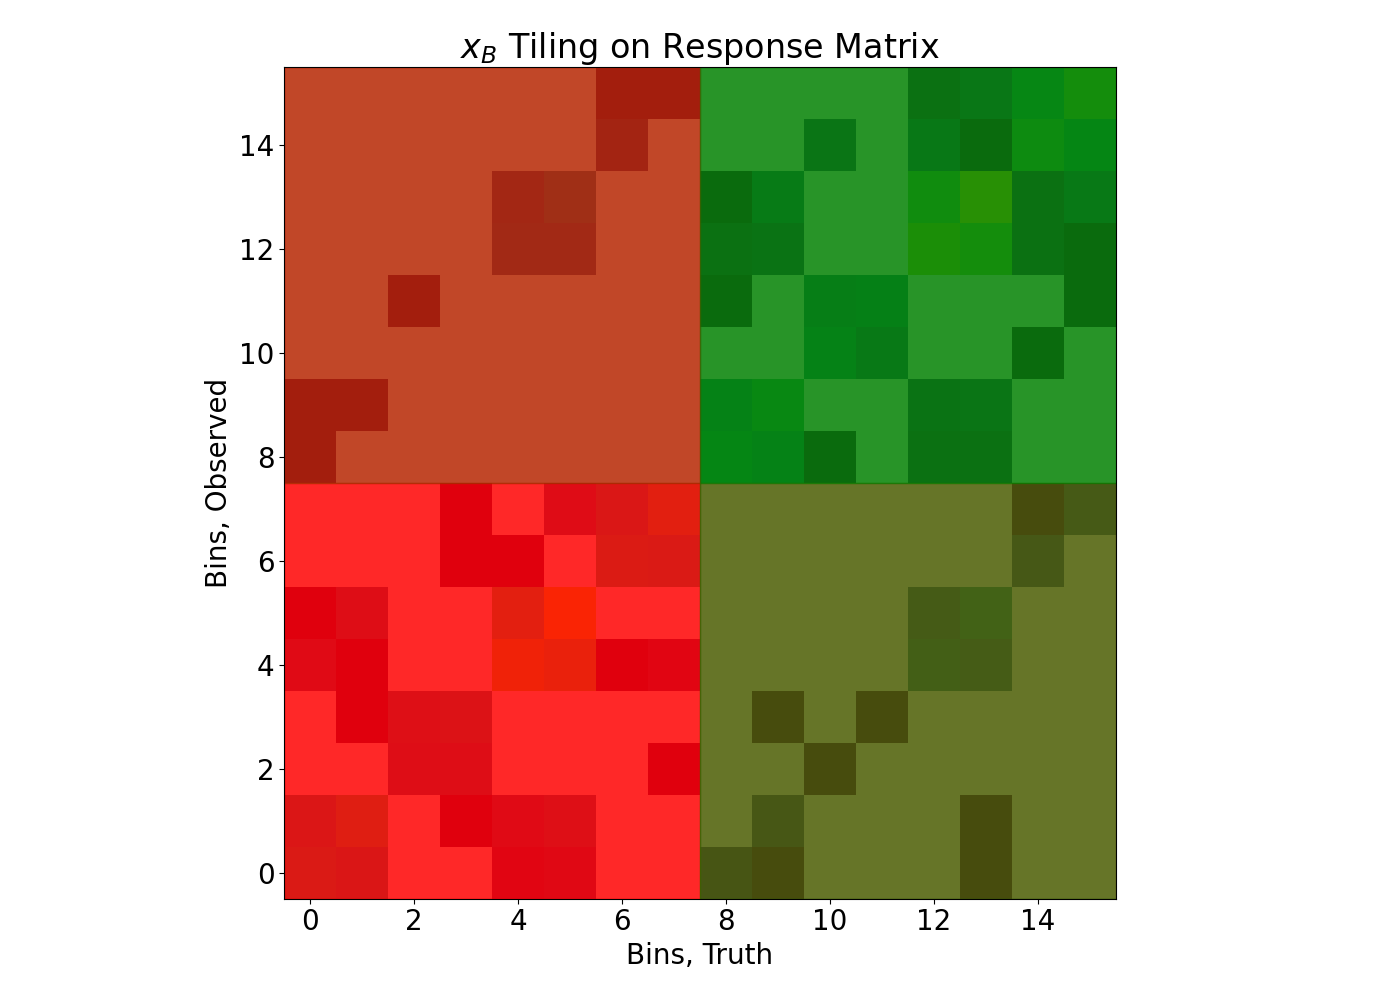
\includegraphics[width=0.479\textwidth]{Chapters/Ch5-Further/0_IBU/pics/4d-2n_example/plaid/4D_2bin_sample_response_matrix_xb.png}
            \label{fig:response_matrix_xb}}
            \hfill
            \subfloat[][Bins are orange if $Q^2$ bin is 0, else blue.]{
            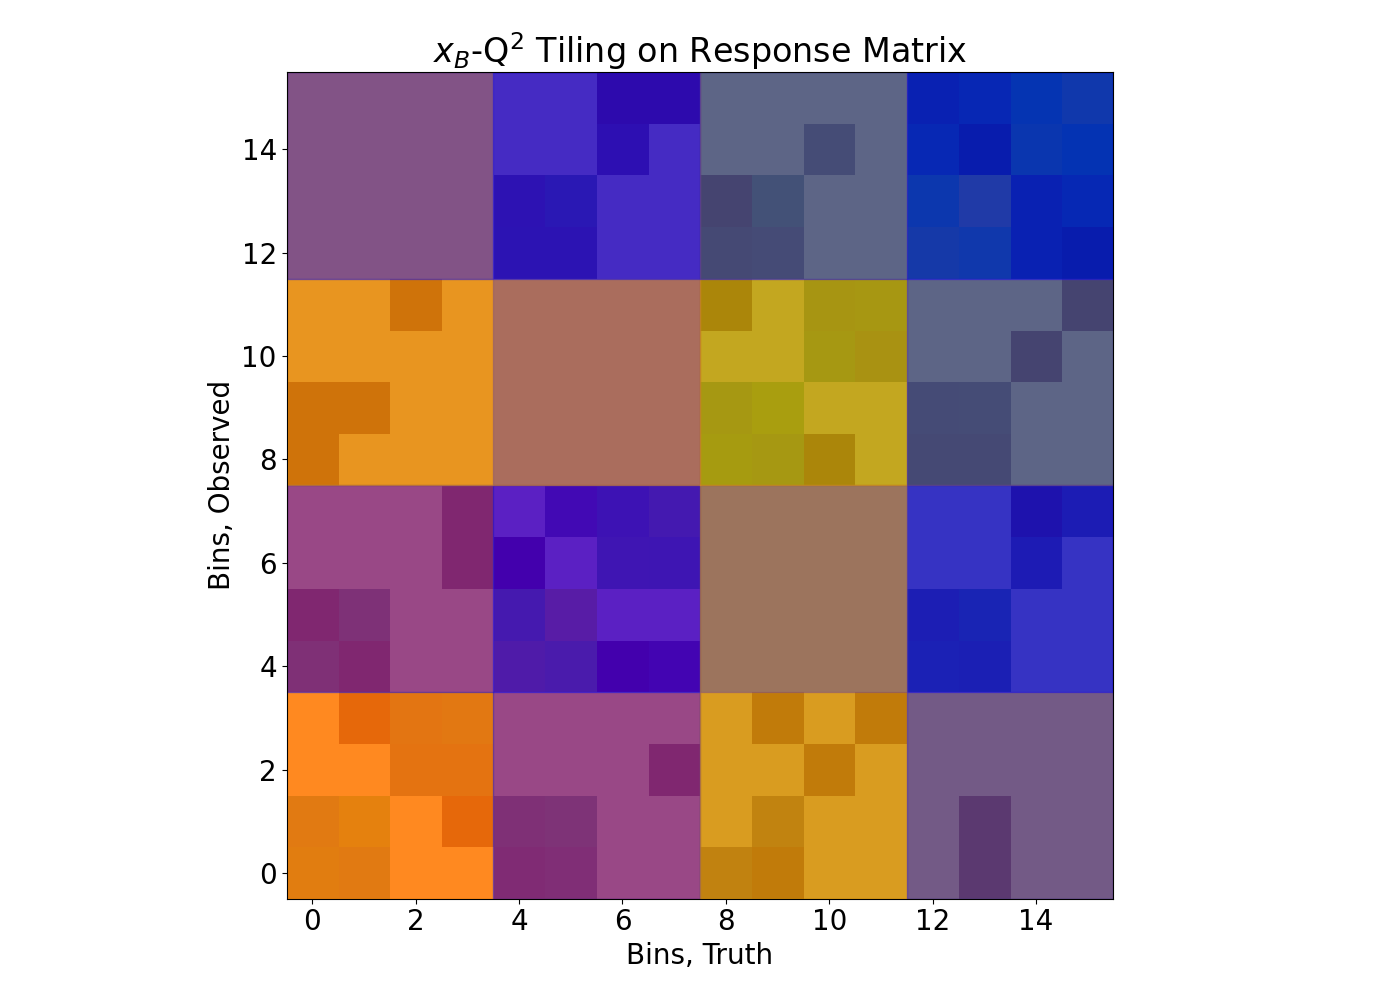
\includegraphics[width=0.479\textwidth]{Chapters/Ch5-Further/0_IBU/pics/4d-2n_example/plaid/4D_2bin_sample_response_matrix_xb_q2.png}
            \label{fig:response_matrix_xb_q2}}
            \\
            \subfloat[][Bins are yellow if $\phi$ bin is 0, else purple.]{
            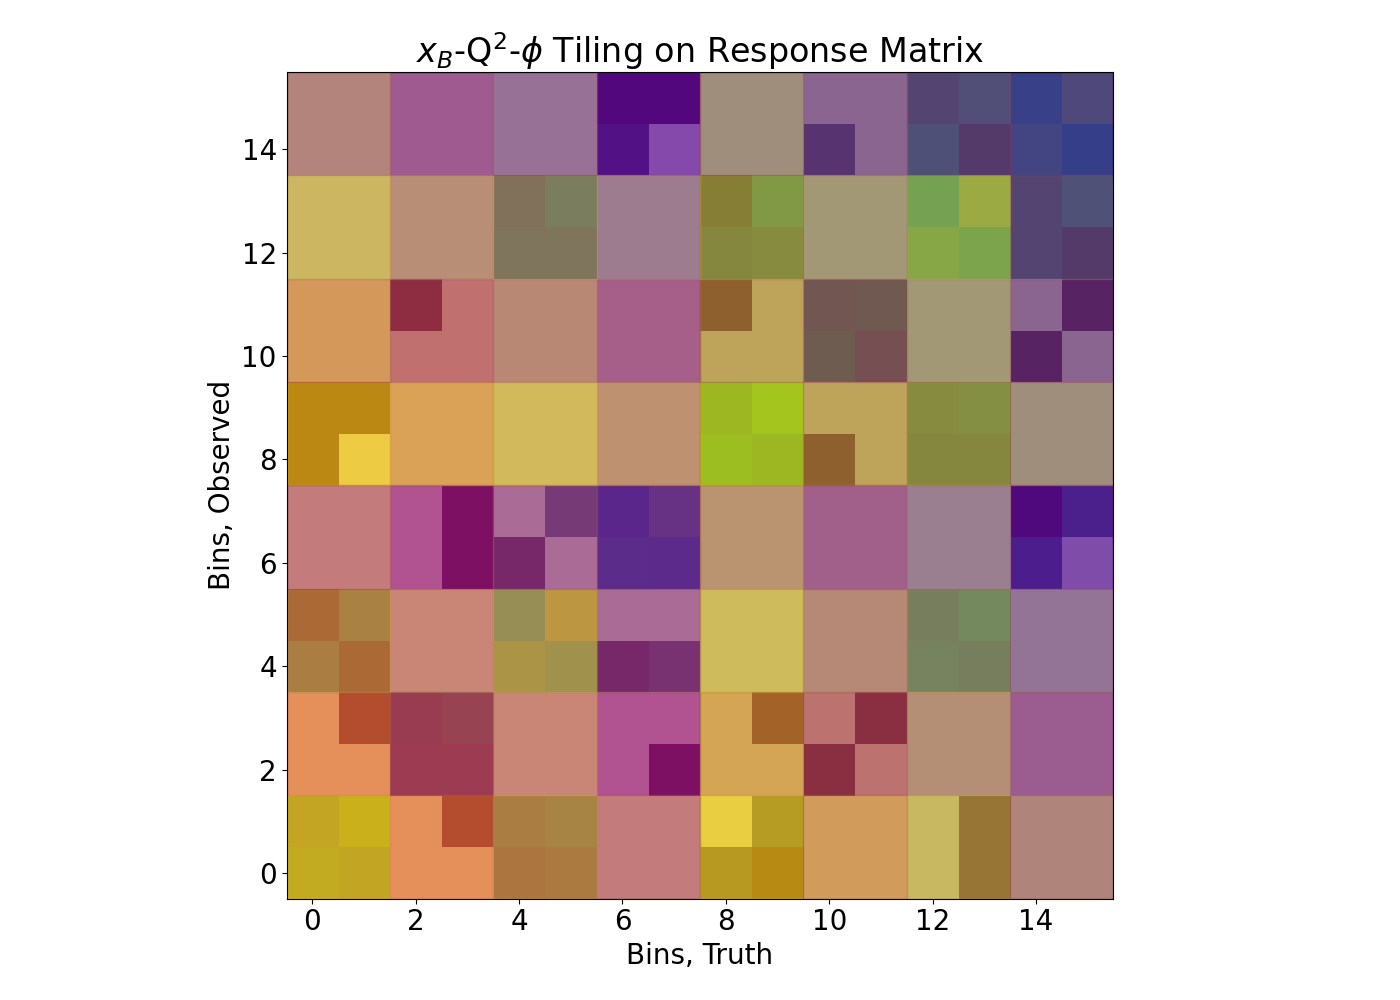
\includegraphics[width=0.479\textwidth]{Chapters/Ch5-Further/0_IBU/pics/4d-2n_example/plaid/4D_2bin_sample_response_matrix_xb_q2_phi.png}
            \label{fig:response_matrix_xb_q2_phi}}
            \hfill
            \subfloat[][Bins are clear if $t$ bin is 0, else dark.]{
            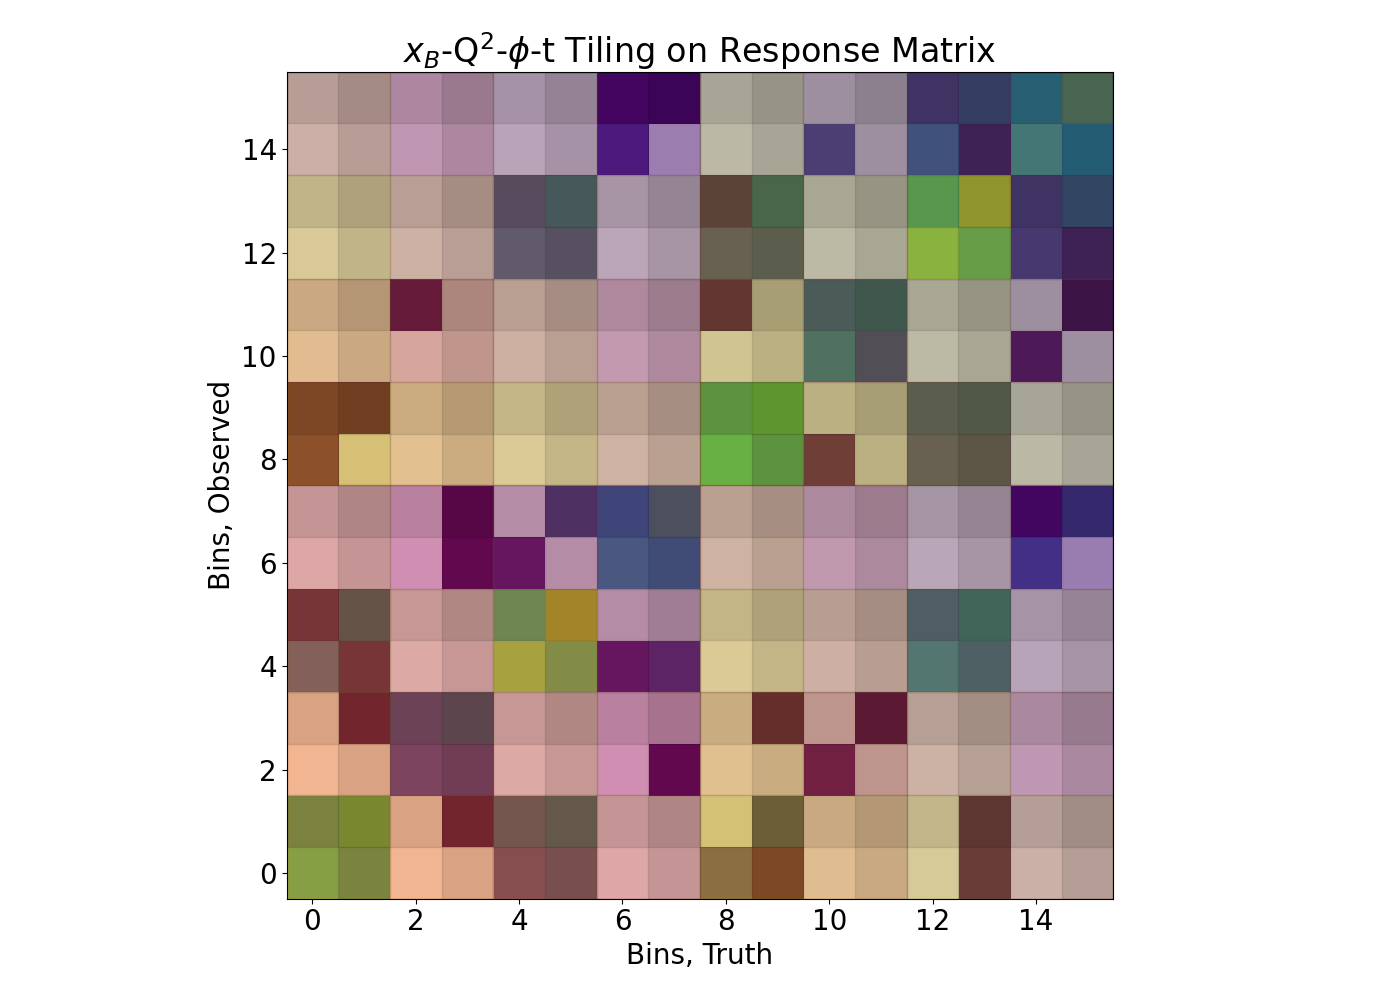
\includegraphics[width=0.479\textwidth]{Chapters/Ch5-Further/0_IBU/pics/4d-2n_example/plaid/4D_2bin_sample_response_matrix_xb_q2_phi_t.png}
            \label{fig:response_matrix_xb_q2_phi_t}}
            \caption[Flattening Map on 4D 2 Bin Example]{Flattening a 2x2x2x2 response matrix can be visualize by successive colorings of columns and rows as a function of their true and observed bin numbers. For each variable, each bin is either number 0 or number 1, eventually leading to 256 uniquely colored bins.}
            \label{fig:unrolling}
        \end{figure}
    
        
        


        This flattening allows for unfolding of arbitrarily high dimensional datasets, although it is drastically more computationally expensive as the number of bins increases. In this case, the unfolding requires the calculation of a multinomial covariance matrix, which in general will take size (number of total bins)$^4$. This analysis has a total of 8x10x8x10 bins across $x_B$,$Q^2$,$\phi$, and t, yielding 6,400 individual bins. This would require a full covariance matrix to have 1.6x10$^{15}$ entries, corresponding to a memory requirement of 12 petabytes, if using 8 byte memory number types. This scaling is illustrated in \figref{fig:ibu_mem_scale}, and means using IBU on the entire dataset space is not possible. 

        \begin{figure}[ht]
            \centering
            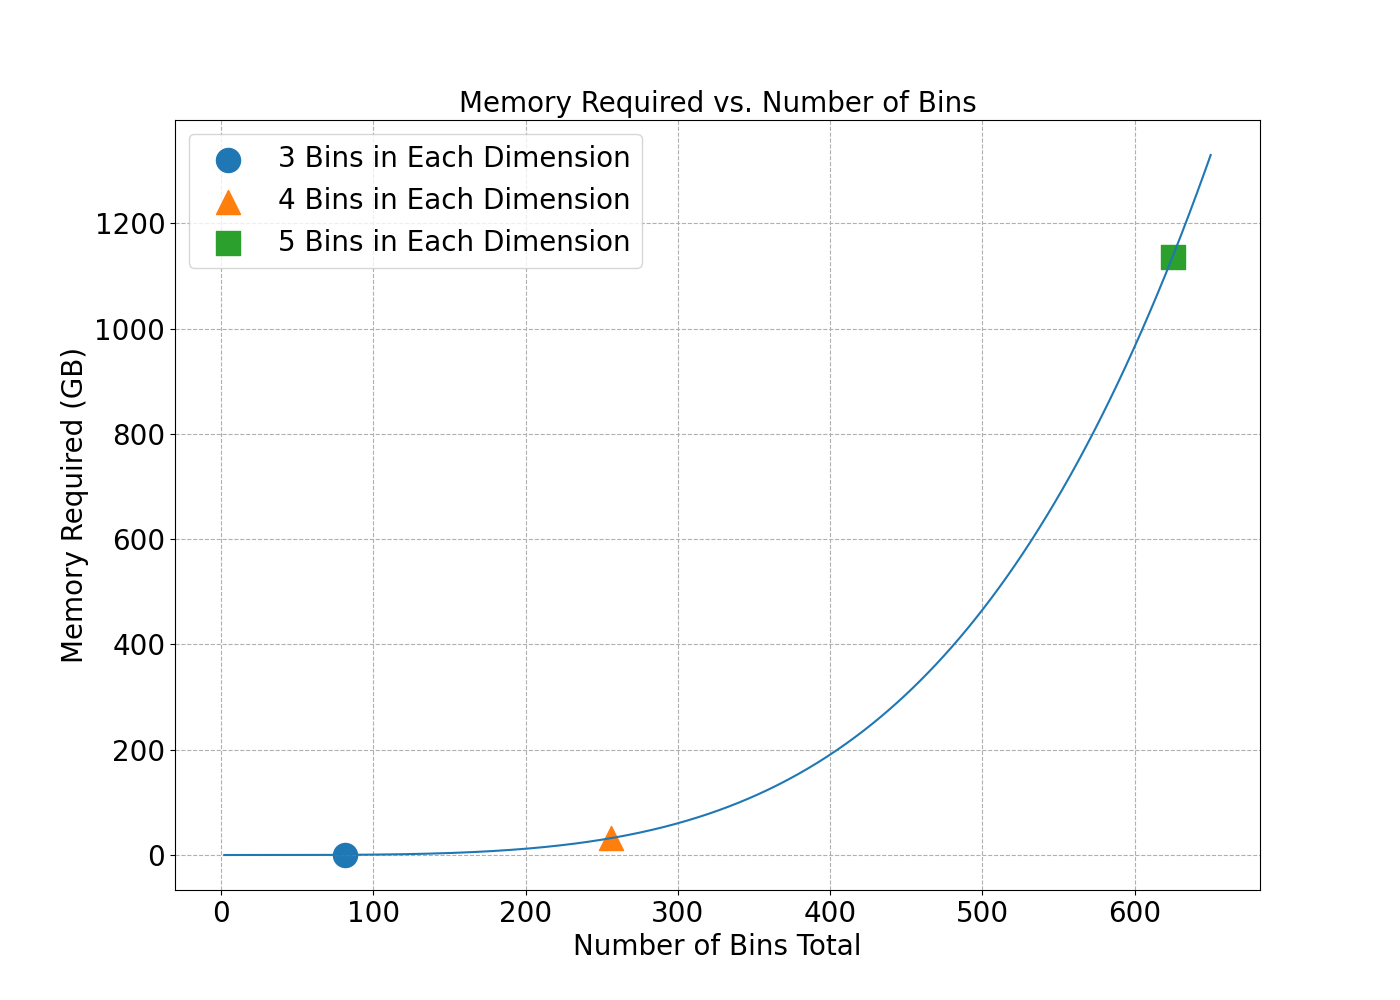
\includegraphics[trim={0 0 0 0},clip,width=0.8\textwidth]{Chapters/Ch5-Further/0_IBU/pics/memory_required_vs_number_of_bins_in_each_dim.png}
            \caption[Memory Requirements of IBU]{Memory Requirements of IBU grow rapidly as a function of bin count, especially in four dimensions. In particular, a multinomial covariance matrix is needed of size ((counts per bin)x(error per bin))x((counts per bin)x(error per bin)), leading to a memory scaling of the 16th power of the number of bins per dimension.}
            \label{fig:ibu_mem_scale}
        \end{figure}


        
        %506 unrolled bins = 506x506 response matrix = 506x506x506x506 matrix = (256036, 256036) = 65554433296 entries with 8 bytes (float64) or 4 bytes (float32) data each, yielding 524435466368 (float64) / 1024\^3 = 488 GiB of memory needed (or 244 for float 32). 
        %This means full matrix would have 8*10*8*10 = 6400 x 6400 response matrix =  6400 x 6400 x  6400 x 6400 cov matrix = 1.6777216e+15 entries = 12207.03125 TiB = 12.2 PiB memory
        
            %In general, the multinomial covariance provides a measure of the uncertainty between different bins in the unfolded result. Each entry in the covariance matrix describes the covariance between two bins - that is, it quantifies how much the two bins are expected to change together due to statistical fluctuations in the data. This is important information when it comes to interpreting the uncertainties on the unfolded distribution.
        

        To remedy this, we can leverage the fact that the response matrix should be block-diagonal if events do not migrate further away than just their immediately neighboring bins. This is physically reasonable, as the resolution width for binning variables is nearly always less than half the width of any variable's bin. Accordingly, we can process our response matrix through a moving window that only calculates bin migrations between neighboring bins. A four dimensional bin has 80 adjacent neighbors ($3^4-1$), which yields a more computationally feasible 81x81 bin response matrix for unfolding. This 3x3x3x3 kernel is then scanned across the entire bin phase space with a stride length of 1, and the individual 81x81 unfolding matrices are stitched together to obtain information over the full space. \figref{fig:ibu_window_1} shows this 3x3x3x3 kernel across $x_B$,$Q^2$ and $\phi$,t and \figref{fig:ibut_scan} illustrates scanning the kernel across $\phi$,t with stride=1.

        \begin{figure}[H]
            \centering
            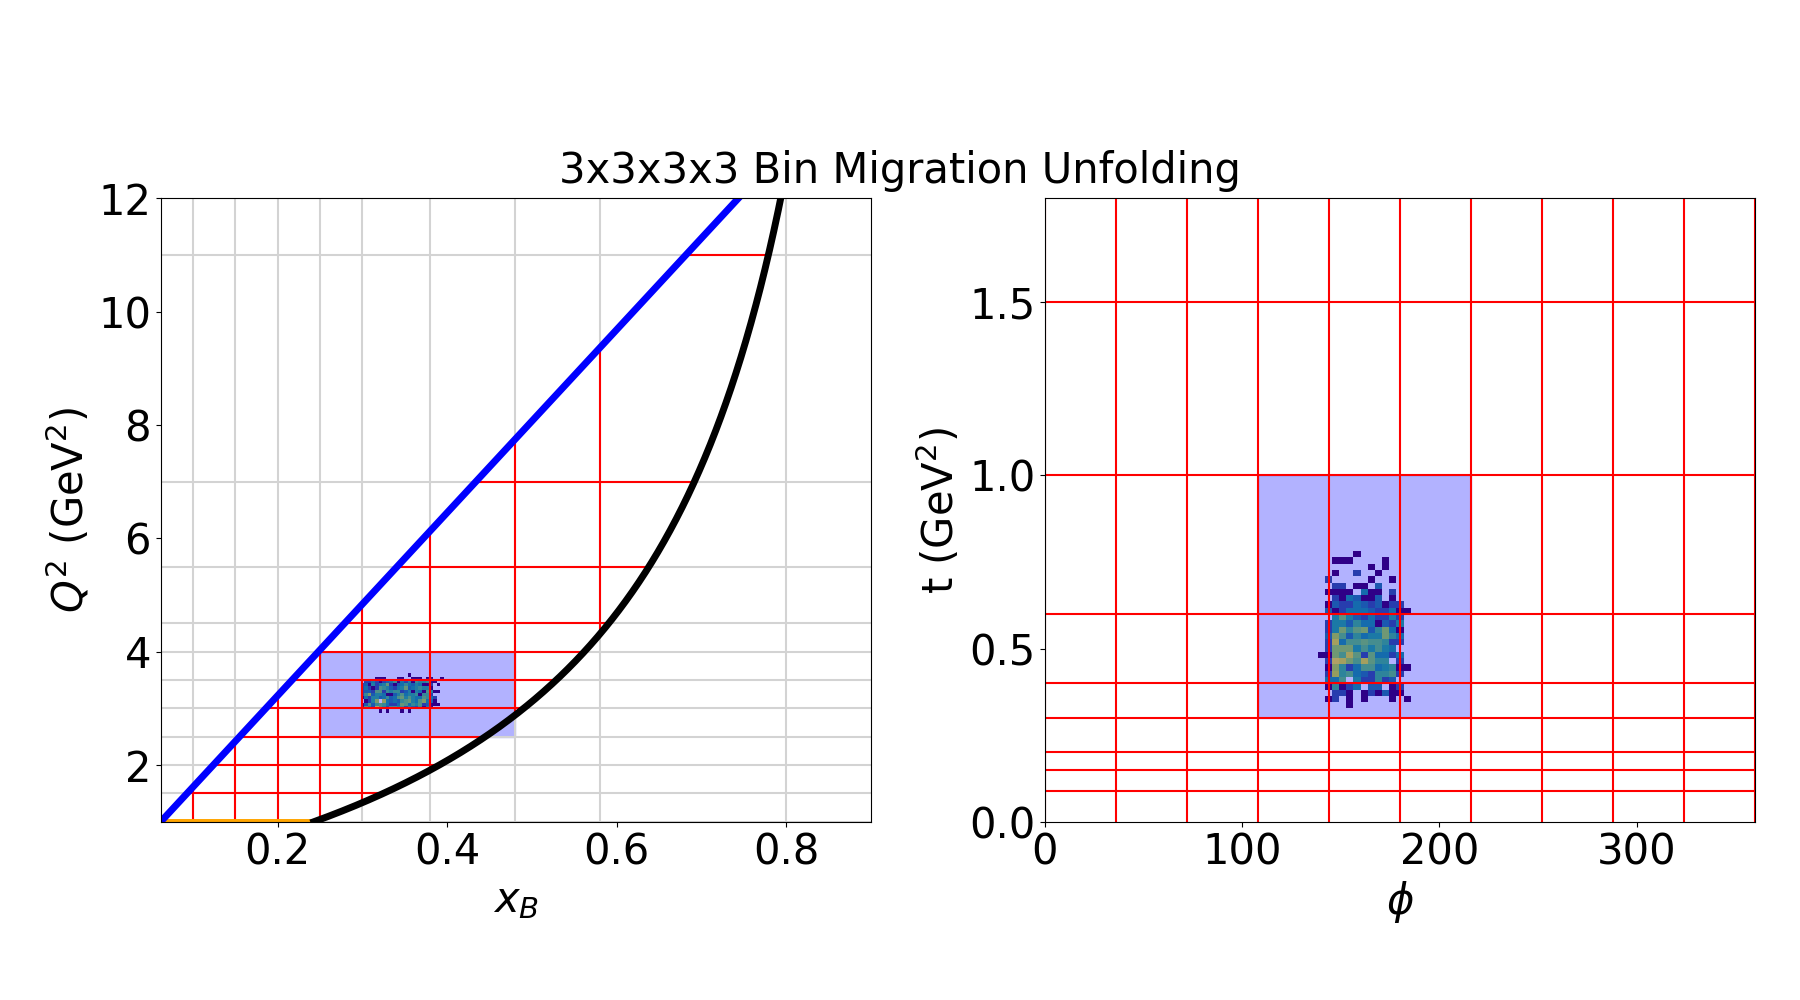
\includegraphics[trim={0 0 0 0},clip,width=.8\textwidth]{Chapters/Ch5-Further/0_IBU/pics/kerneling/bin_migration_1_1_1_1.png}
            \caption[3x3x3x3 Binning Kernel]{3x3x3x3 Binning Kernel across  $x_B$,$Q^2$ (left) and $\phi$,t. }
            \label{fig:ibu_window_1}
        \end{figure}
        
        
        \begin{figure}[H]
            \centering
            \subfloat{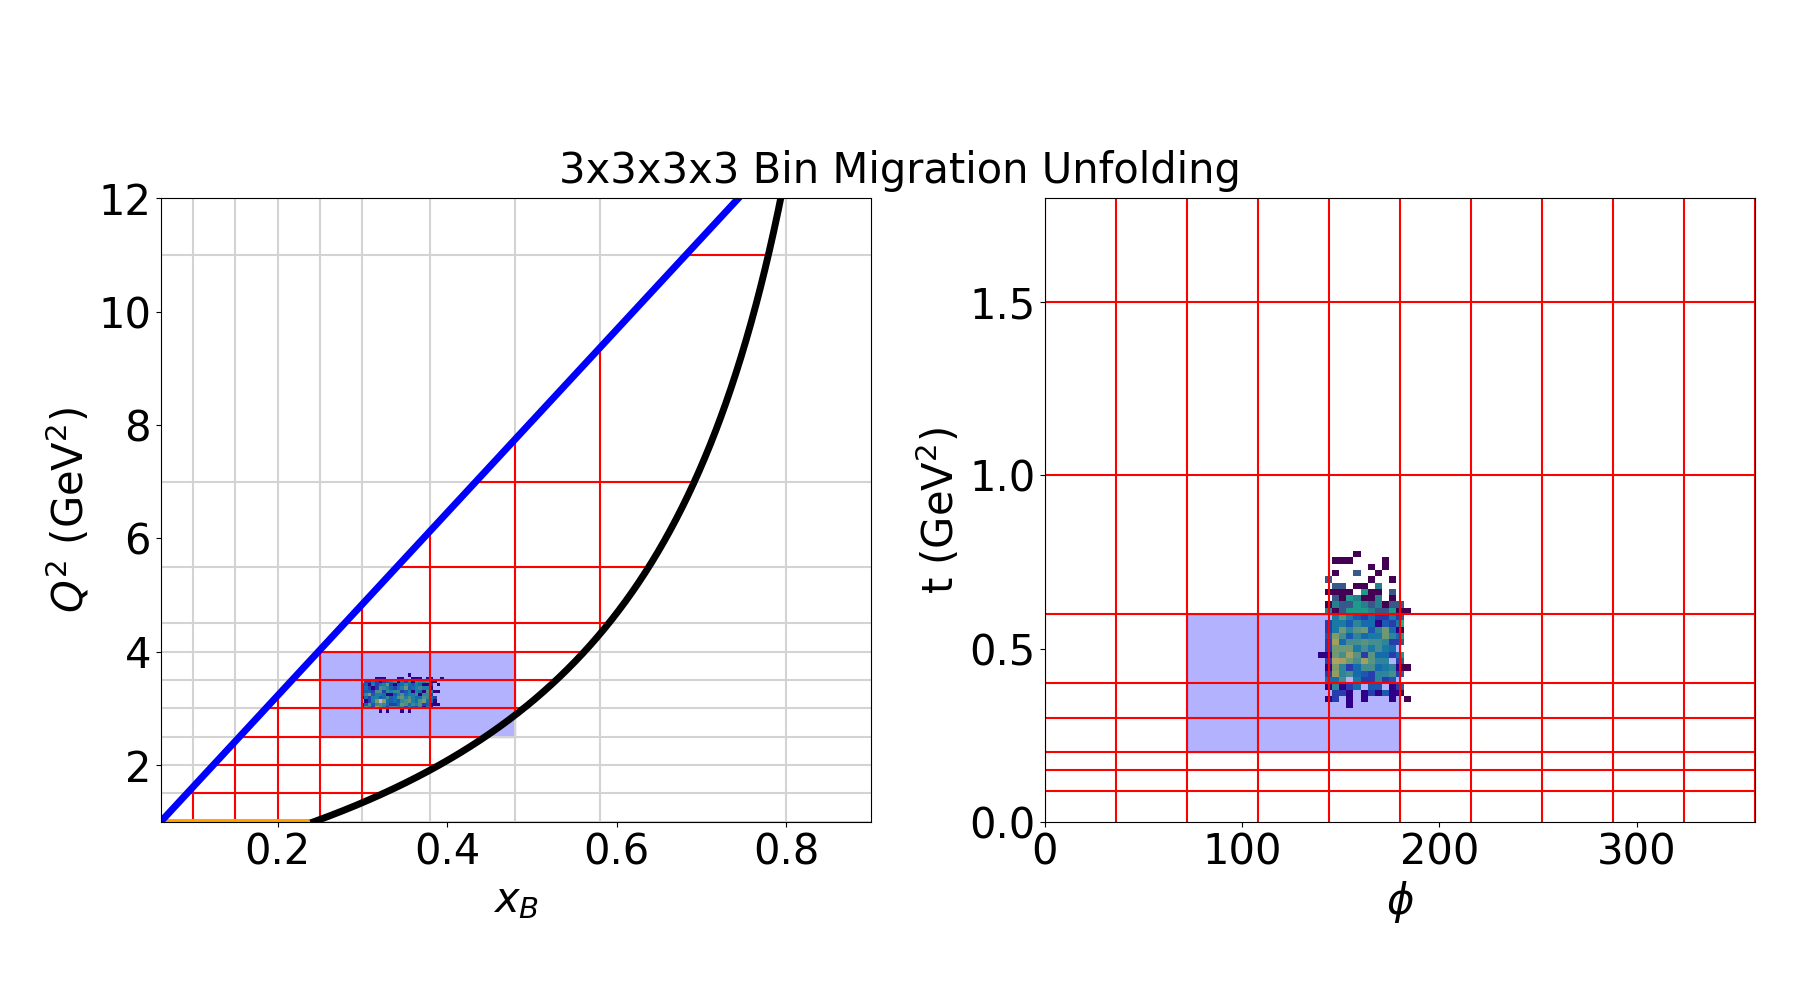
\includegraphics[trim={22.5cm 0 0 5cm},clip,width=0.3\textwidth]{Chapters/Ch5-Further/0_IBU/pics/kerneling/bin_migration_1_1_2_2.png}}
            \subfloat{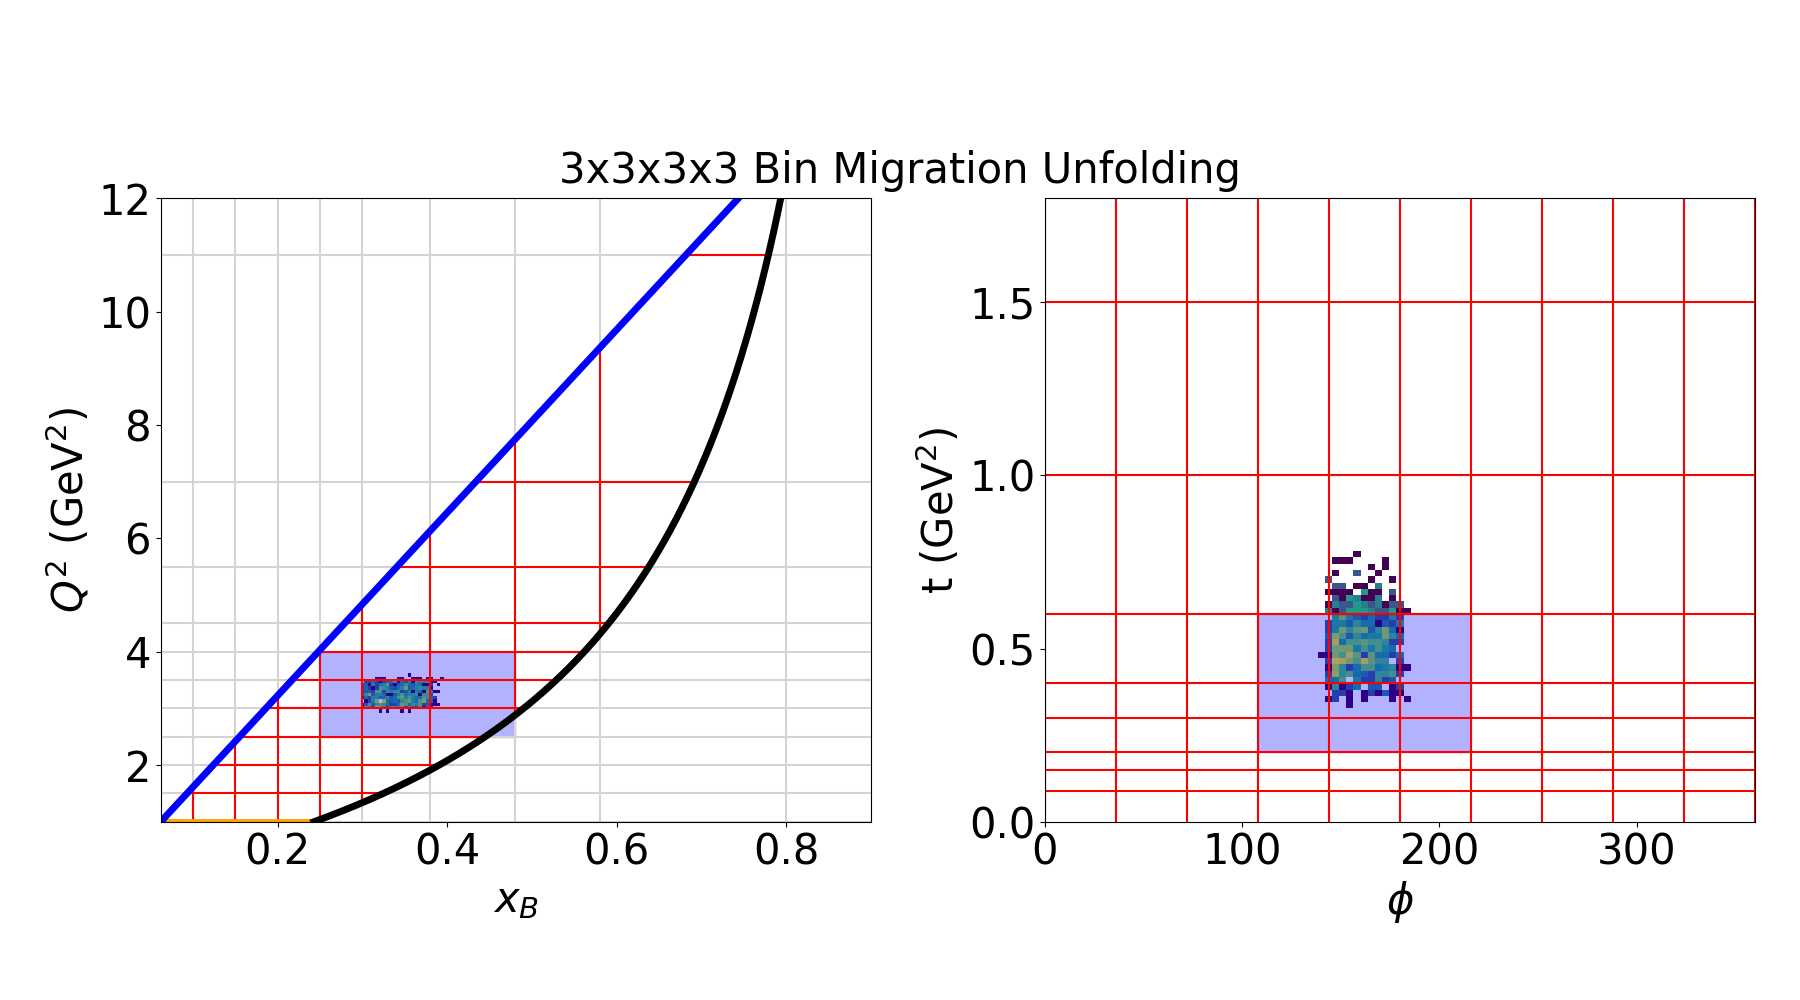
\includegraphics[trim={22.5cm 0 0 5cm},clip,width=0.3\textwidth]{Chapters/Ch5-Further/0_IBU/pics/kerneling/bin_migration_1_1_2_1.png}}
            \subfloat{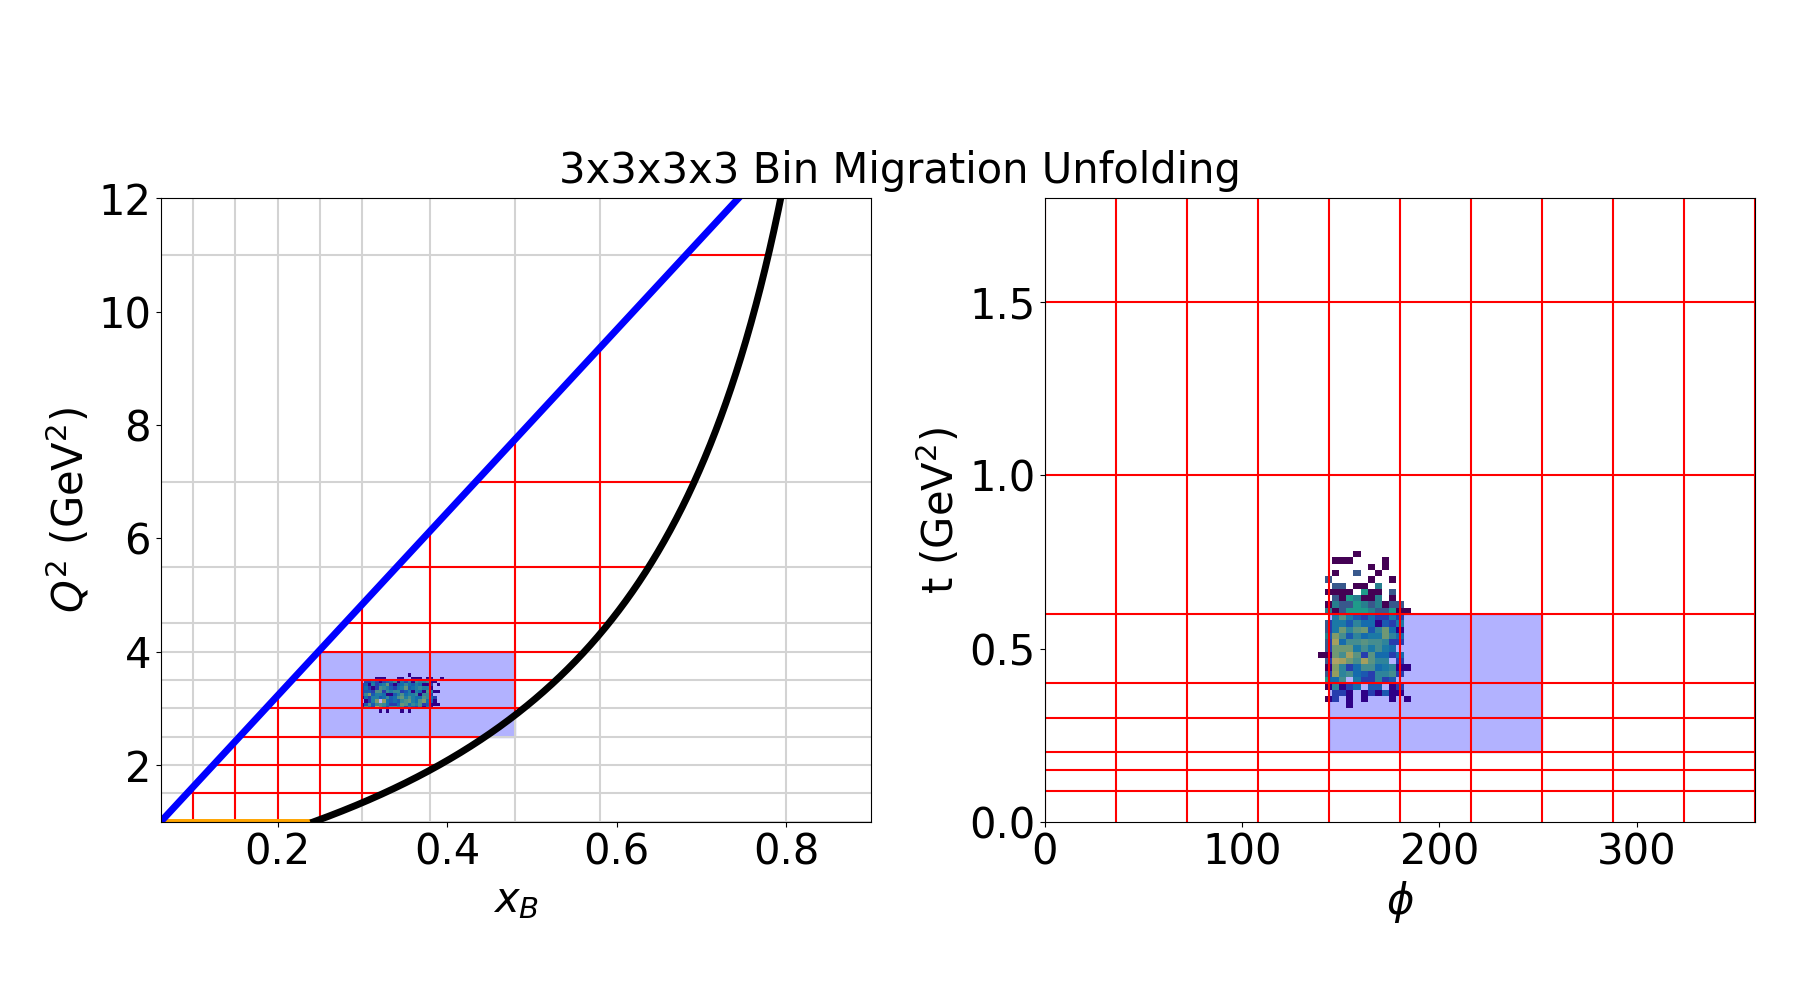
\includegraphics[trim={22.5cm 0 0 5cm},clip,width=0.3\textwidth]{Chapters/Ch5-Further/0_IBU/pics/kerneling/bin_migration_1_1_2_0.png}}\\
            \subfloat{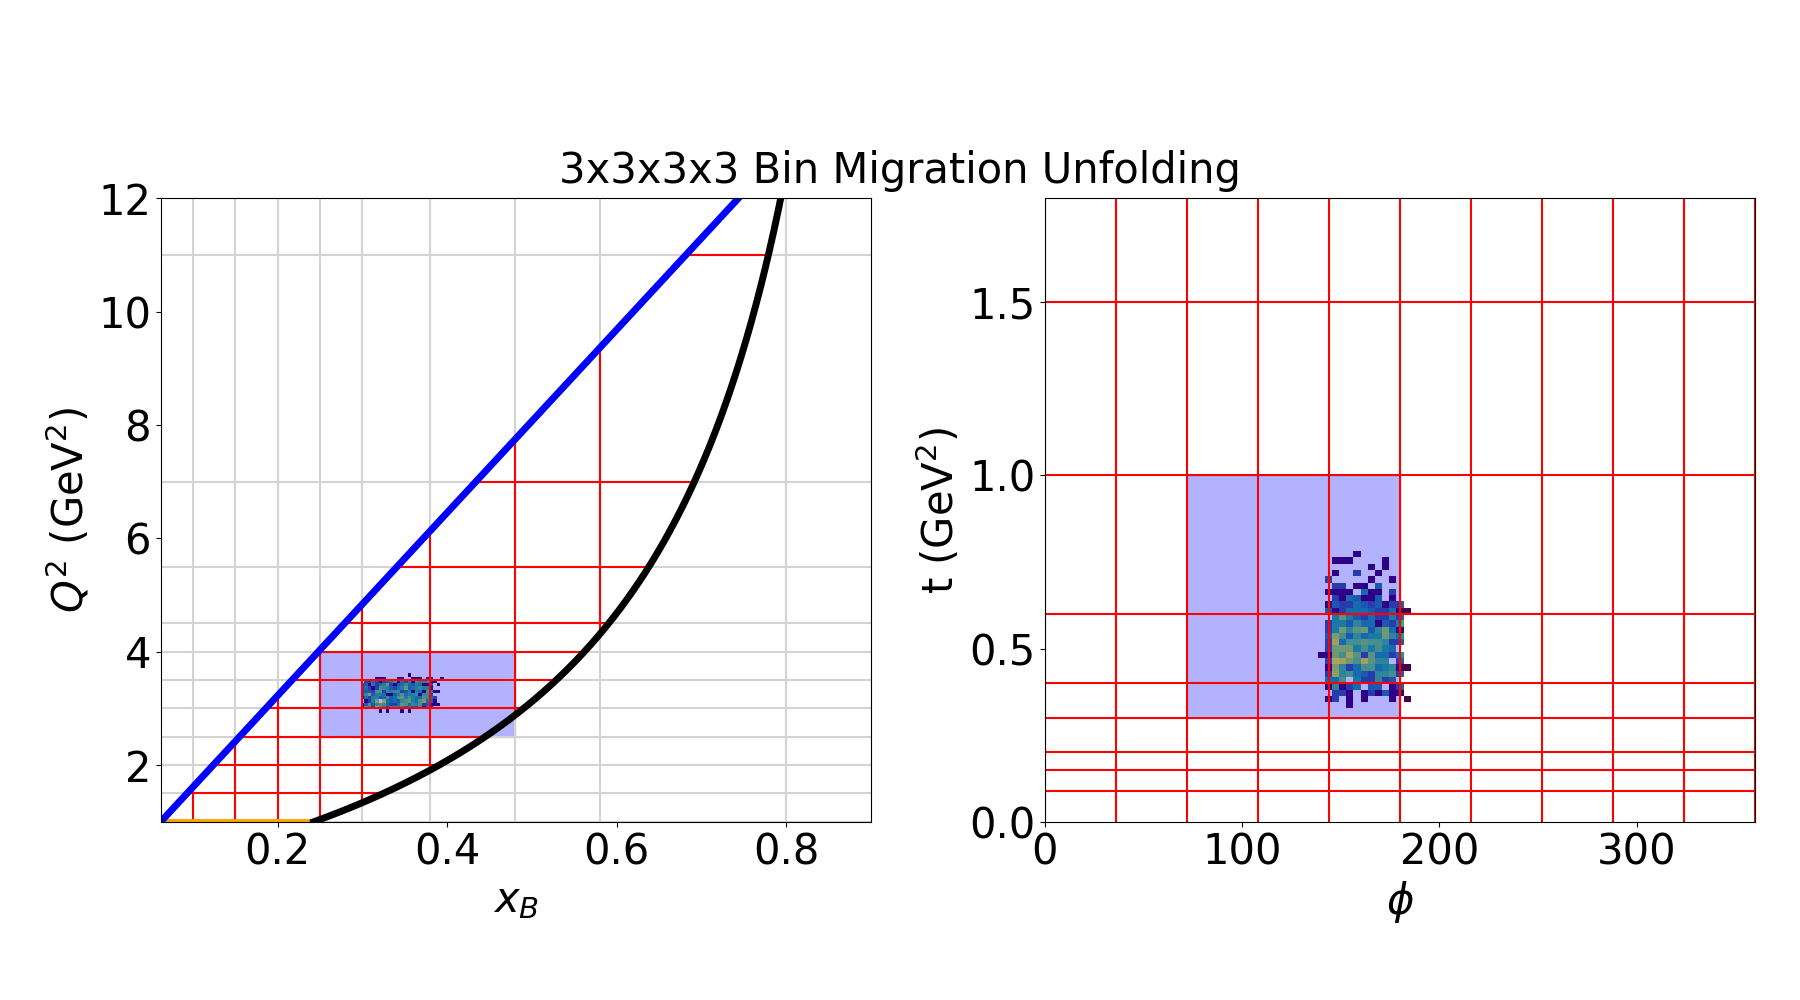
\includegraphics[trim={22.5cm 0 0 5cm},clip,width=0.3\textwidth]{Chapters/Ch5-Further/0_IBU/pics/kerneling/bin_migration_1_1_1_2.png}}
            \subfloat{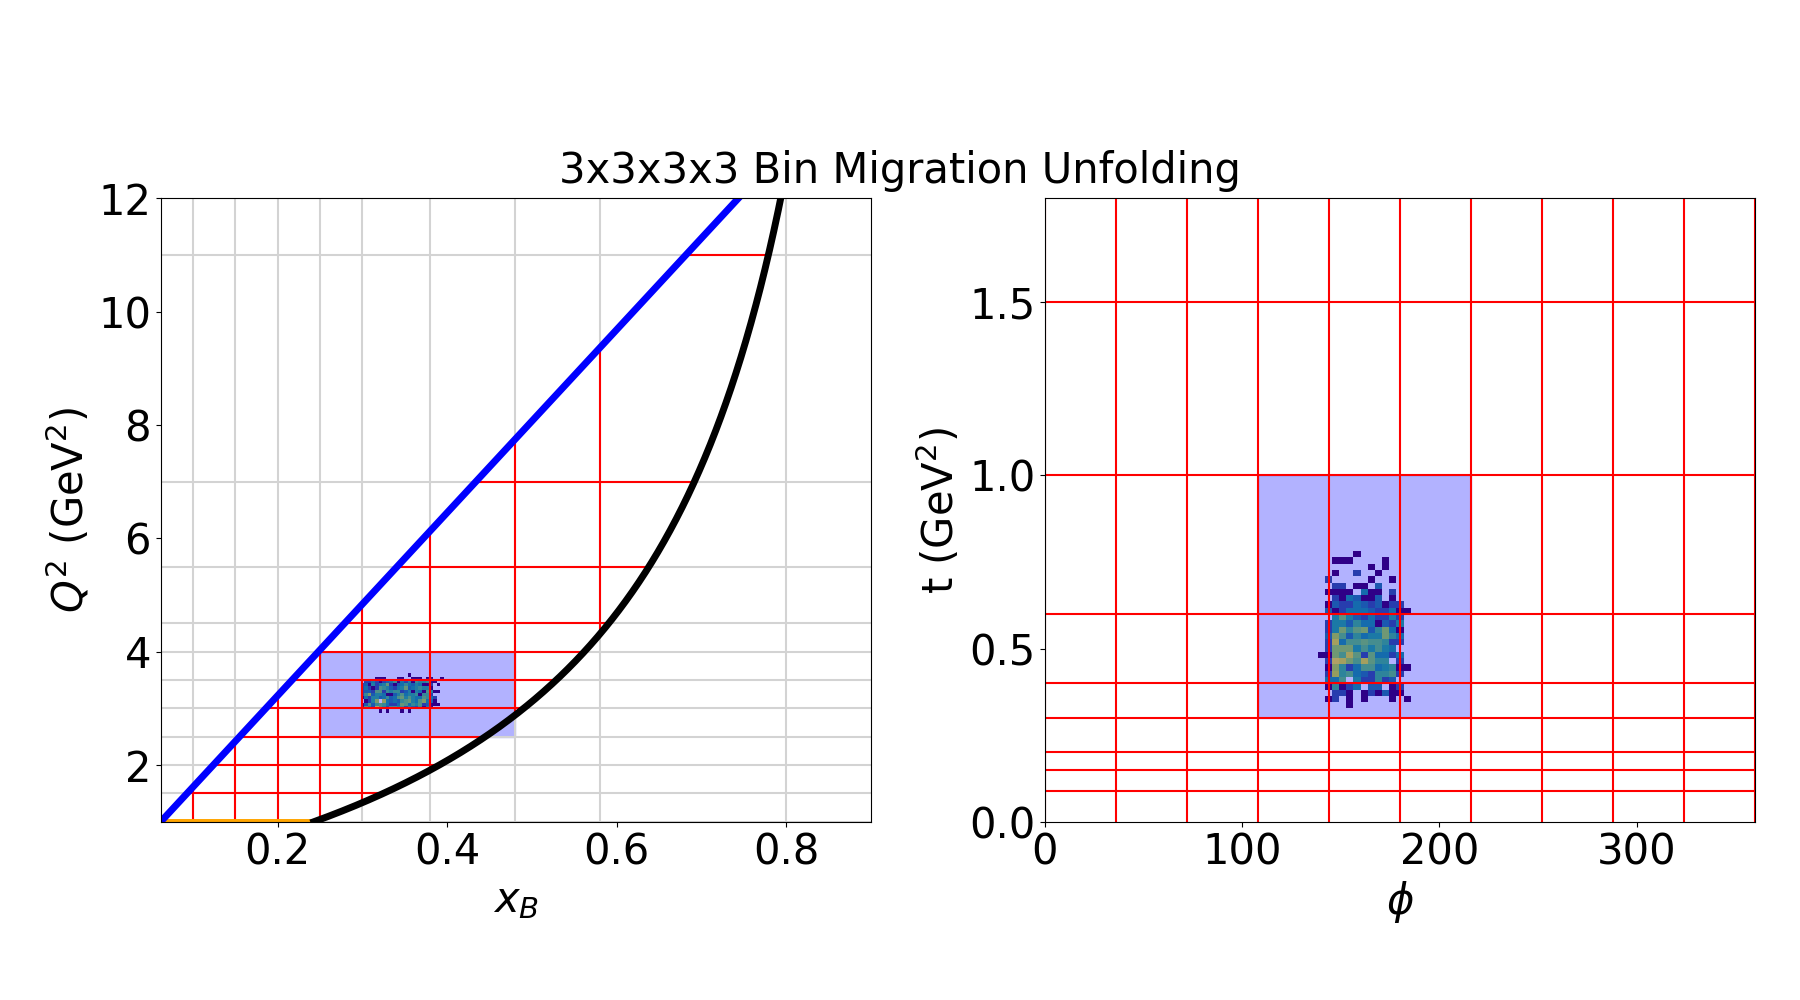
\includegraphics[trim={22.5cm 0 0 5cm},clip,width=0.3\textwidth]{Chapters/Ch5-Further/0_IBU/pics/kerneling/bin_migration_1_1_1_1.png}}
            \subfloat{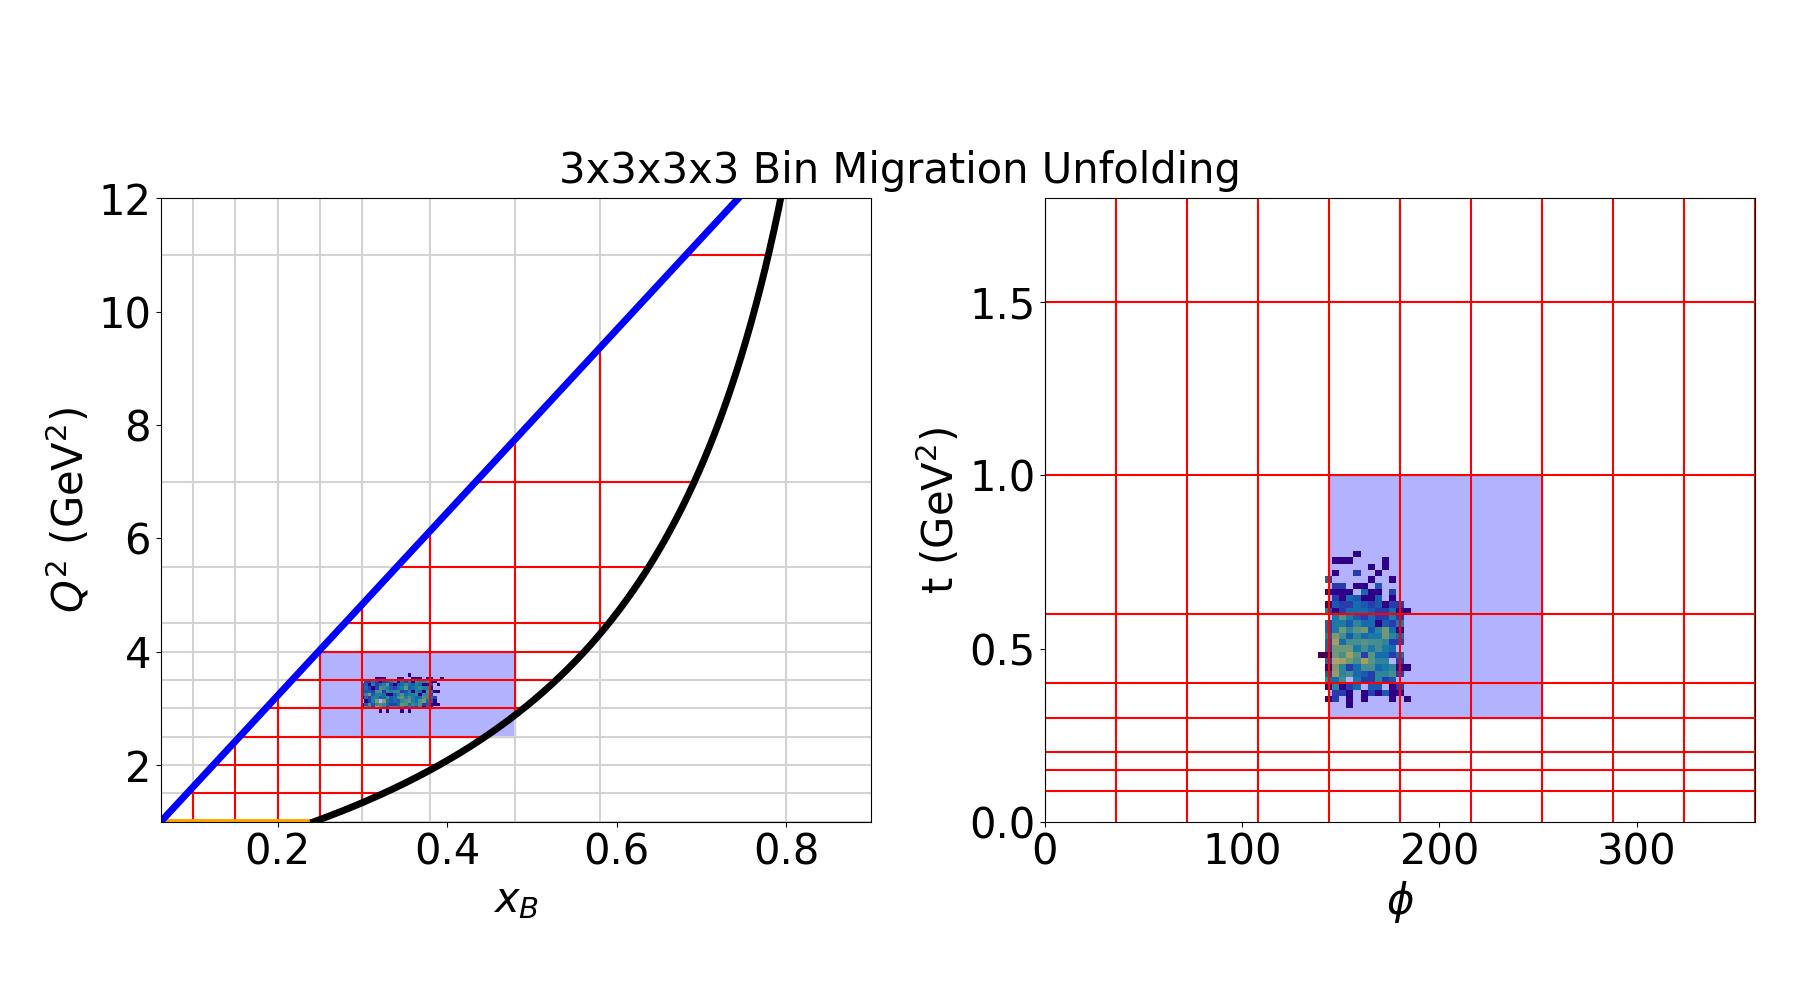
\includegraphics[trim={22.5cm 0 0 5cm},clip,width=0.3\textwidth]{Chapters/Ch5-Further/0_IBU/pics/kerneling/bin_migration_1_1_1_0.png}}\\
            \subfloat{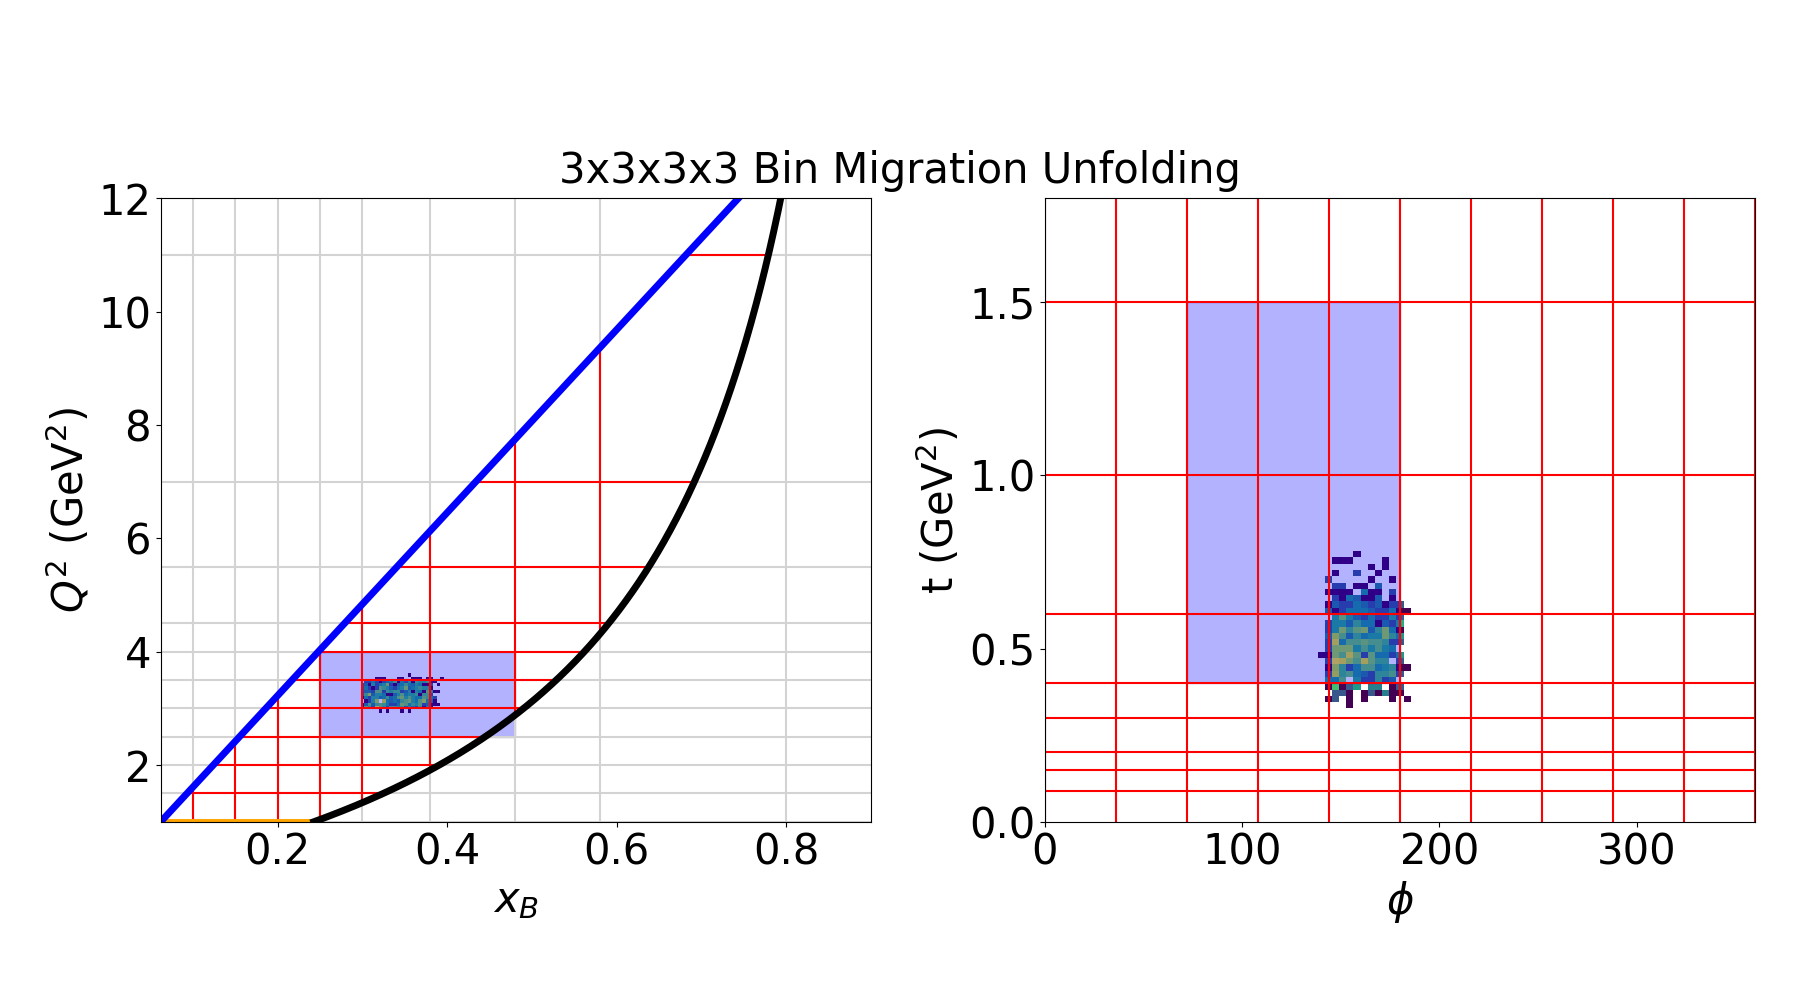
\includegraphics[trim={22.5cm 0 0 5cm},clip,width=0.3\textwidth]{Chapters/Ch5-Further/0_IBU/pics/kerneling/bin_migration_1_1_0_2.png}}
            \subfloat{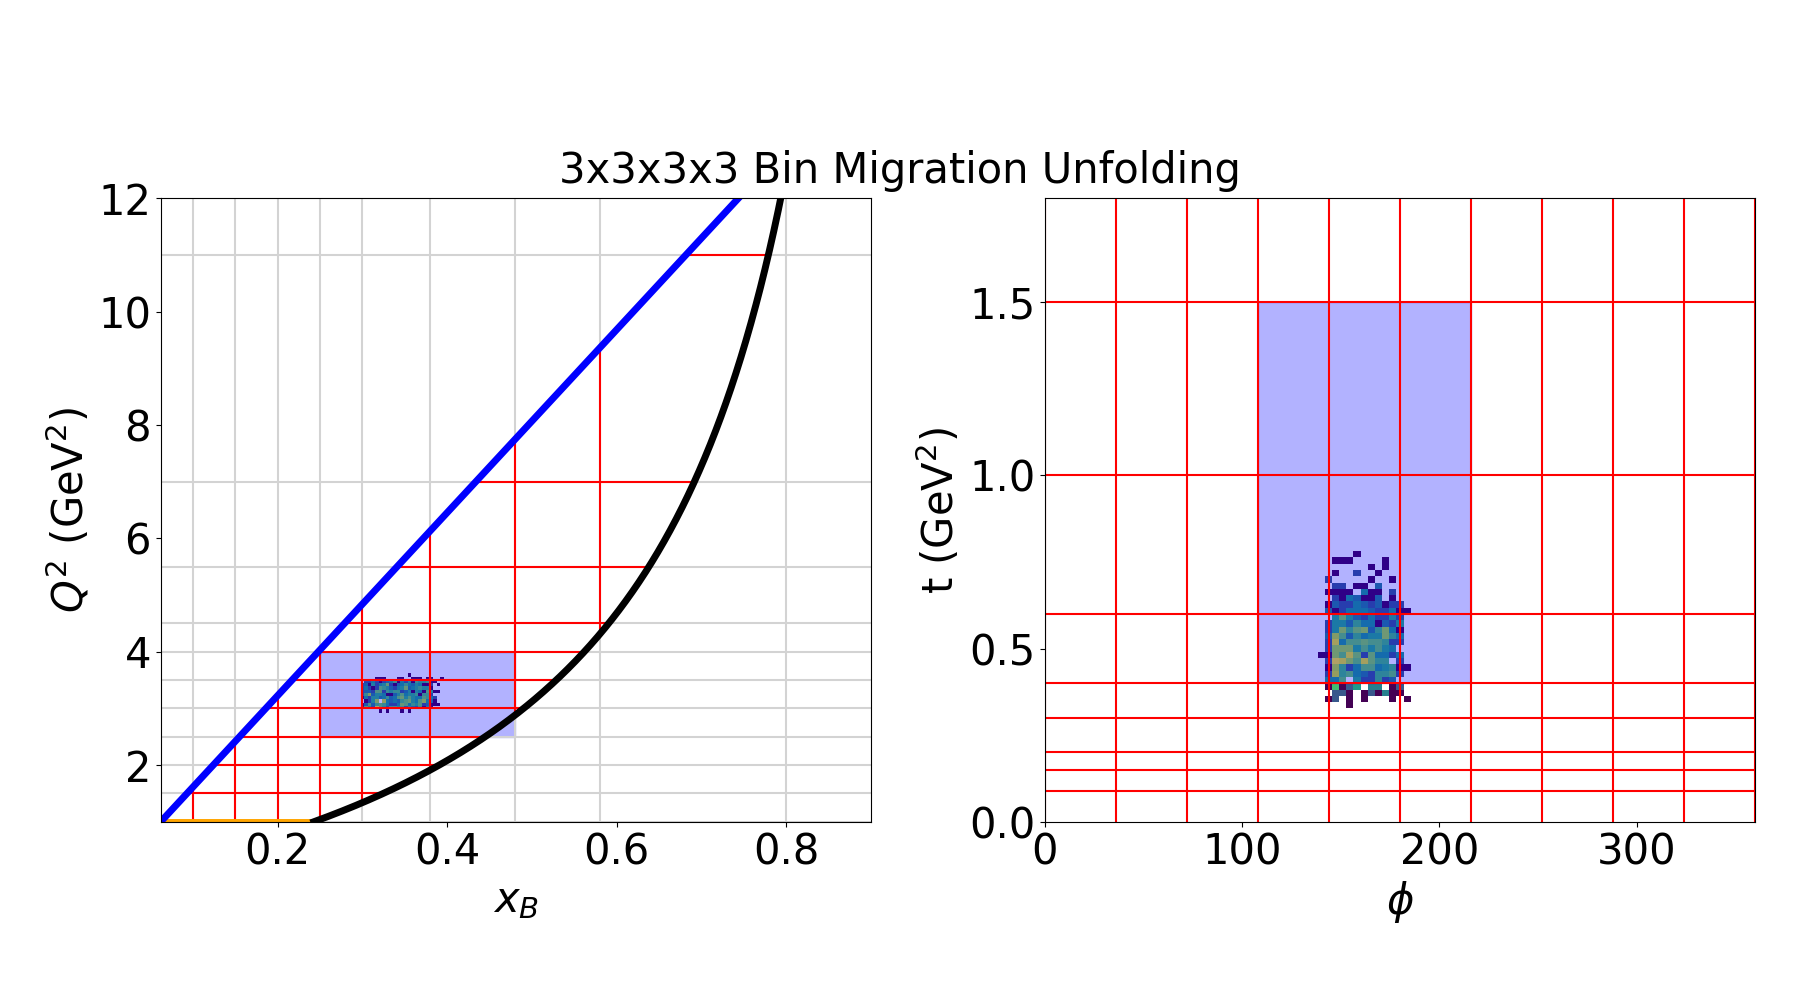
\includegraphics[trim={22.5cm 0 0 5cm},clip,width=0.3\textwidth]{Chapters/Ch5-Further/0_IBU/pics/kerneling/bin_migration_1_1_0_1.png}}
            \subfloat{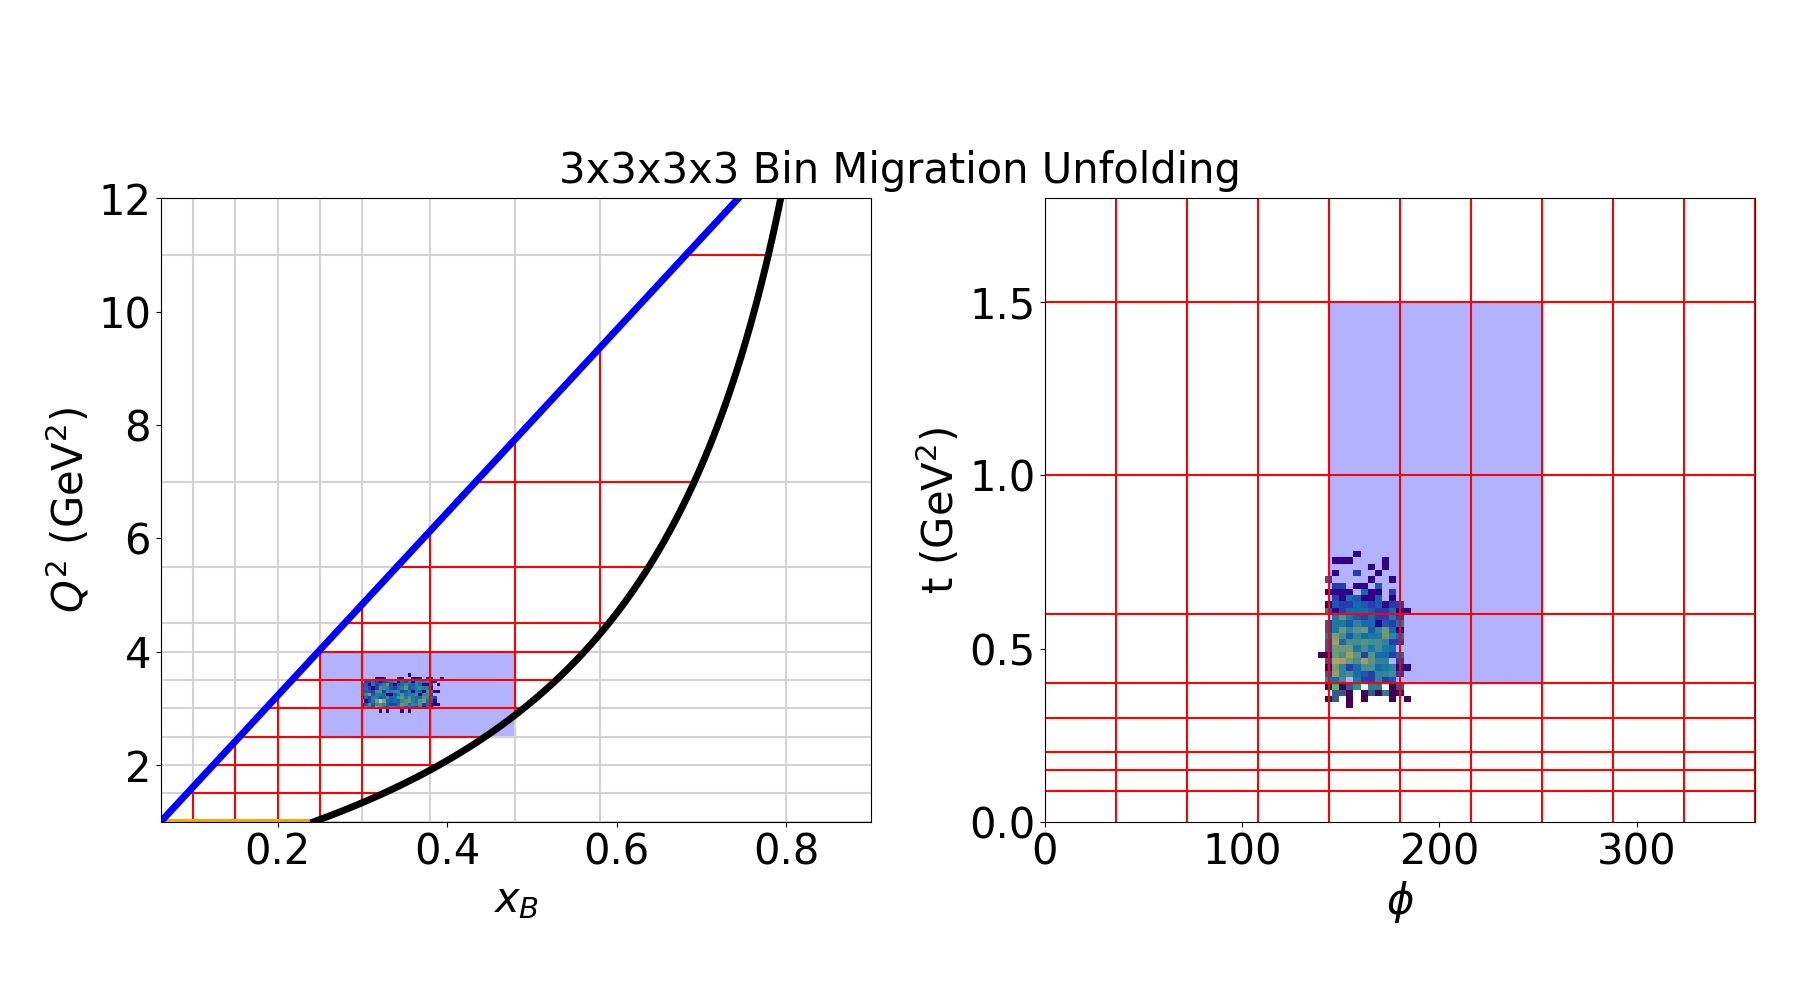
\includegraphics[trim={22.5cm 0 0 5cm},clip,width=0.3\textwidth]{Chapters/Ch5-Further/0_IBU/pics/kerneling/bin_migration_1_1_0_0.png}}\\
            \caption[Kernel Stride Across $\phi$,t]{The kernel is scanned across all binning dimensions with a stride of 1, here illustrated for 9 strides around a central bin in $\phi$,t.}
            \label{fig:ibut_scan}
        \end{figure}


        For each kernel, iterative unfolding was performed with a stopping criterion of 0.00005, which was emperically determined to be the smallest possible that lead to reasonable computing times and results. The use of a uniform prior and Jeffreys prior were compared, but no significant difference was observed so a uniform prior was used for production runs for ease of computation. The kernel stride was wrapped to ensure migrations between very low and high values of $\phi$ were accounted for. 

        
        


    \subsection{Verification of Method}

            \figref{fig:ibu_toy} shows data and results for a test 2x2x2x2 unfolding procedure. The unfolded results coincide closely with the true data distribution. 
    
        \begin{figure}[ht]
            \centering
            \subfloat[][Response matrix.]{
            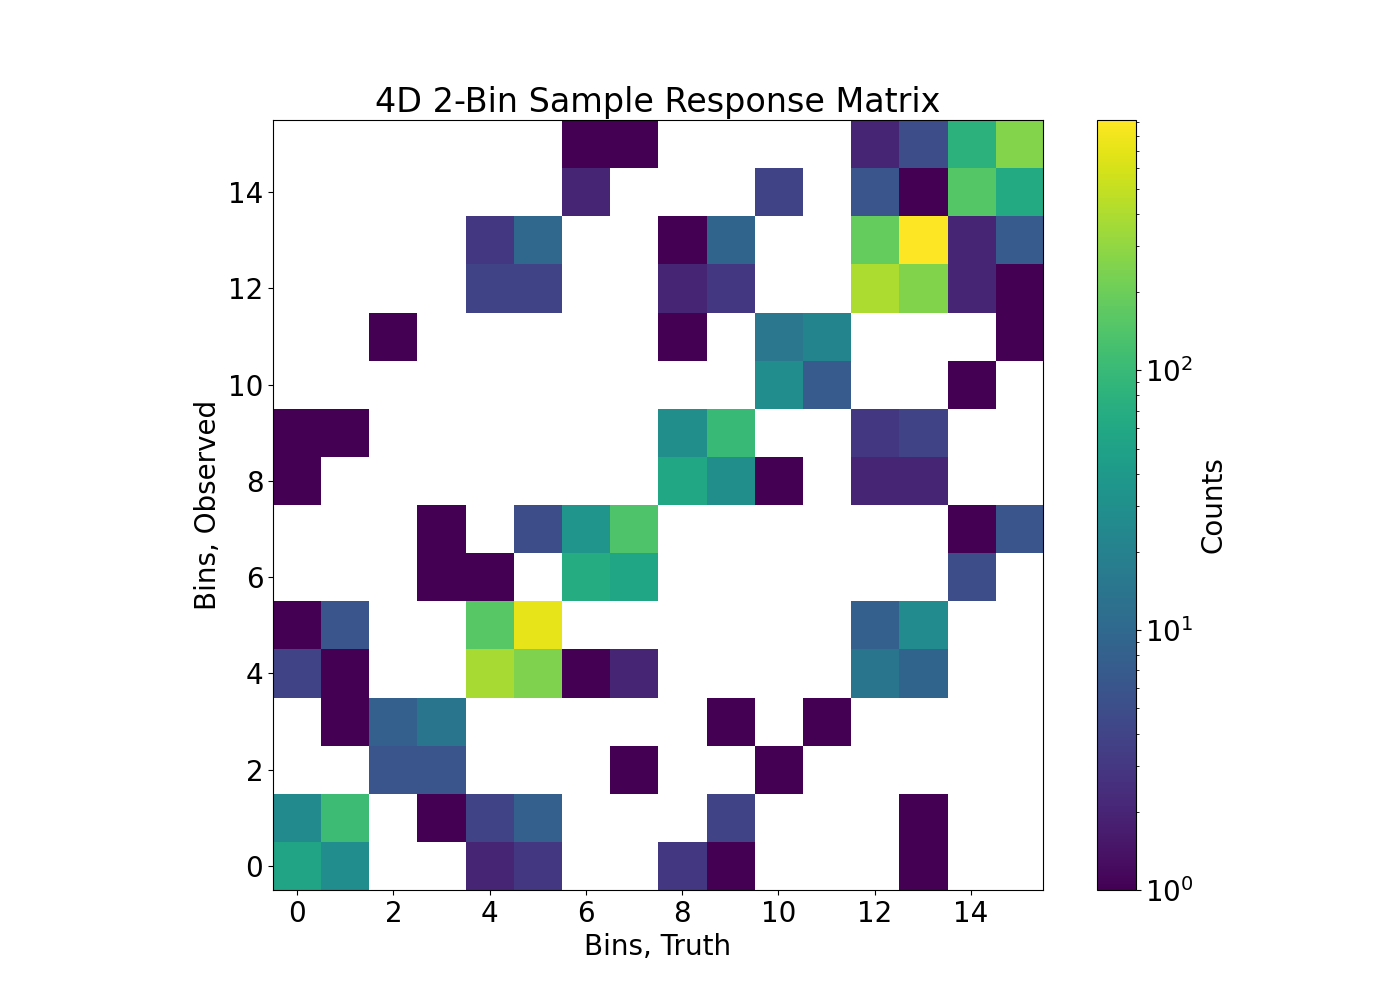
\includegraphics[width=0.449\textwidth]{Chapters/Ch5-Further/0_IBU/pics/4d-2n_example/4D_2bin_sample_response_matrix.png}
            \label{fig:ibu_toya}}
            \hfill
            \subfloat[][True and observed distributions.]{
            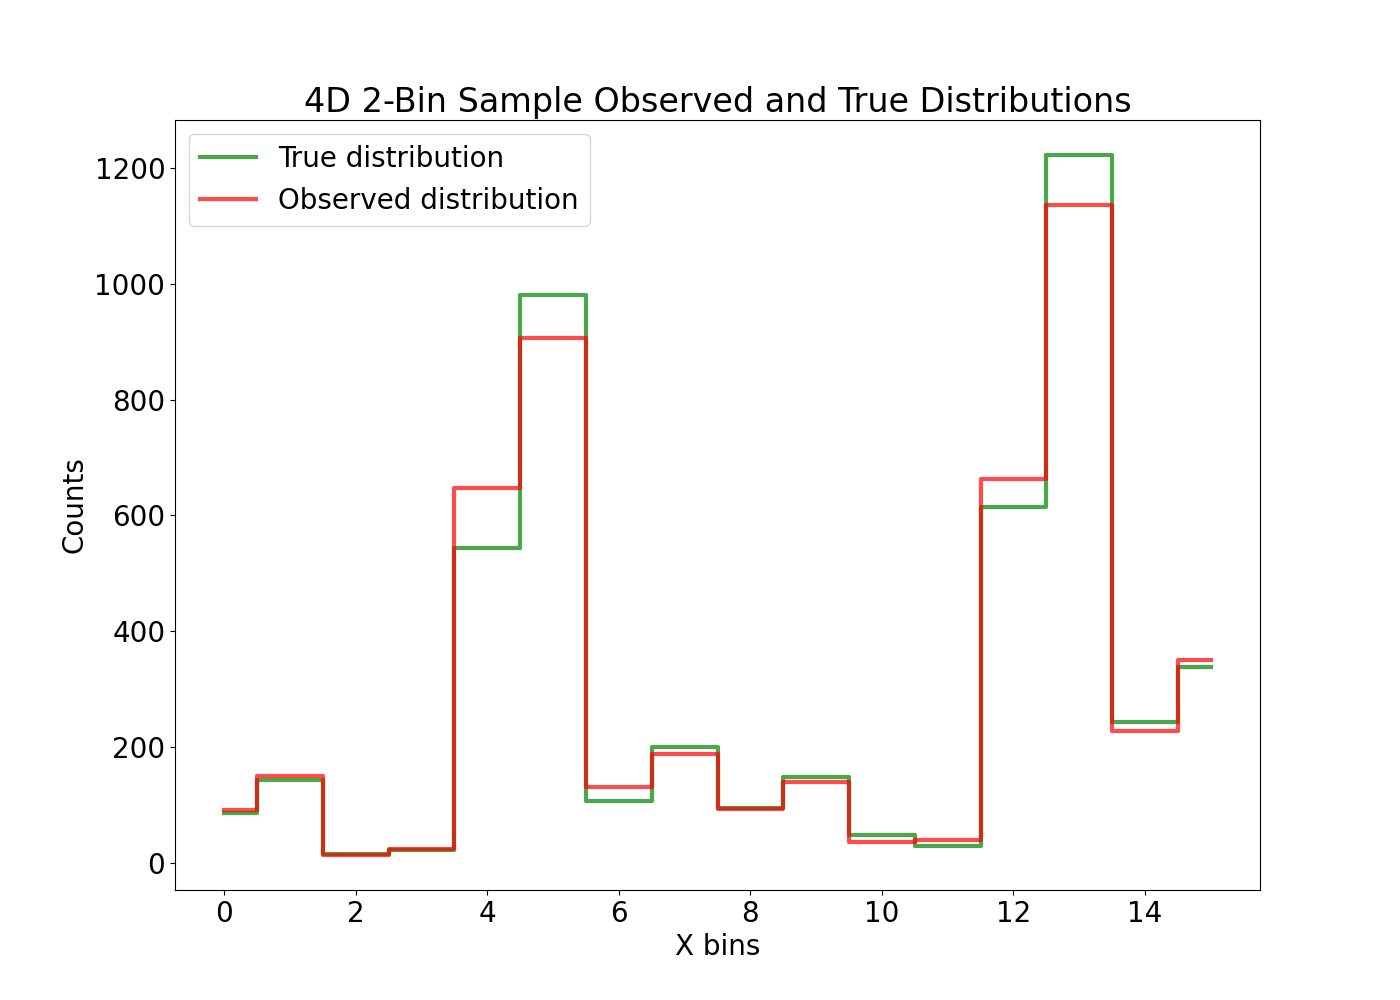
\includegraphics[width=0.449\textwidth]{Chapters/Ch5-Further/0_IBU/pics/4d-2n_example/4D_2bin_sample_observed_and_true_distributions.png}
            \label{fig:ibu_toyb}}
            \\
            \subfloat[][Normalized response matrix.]{
            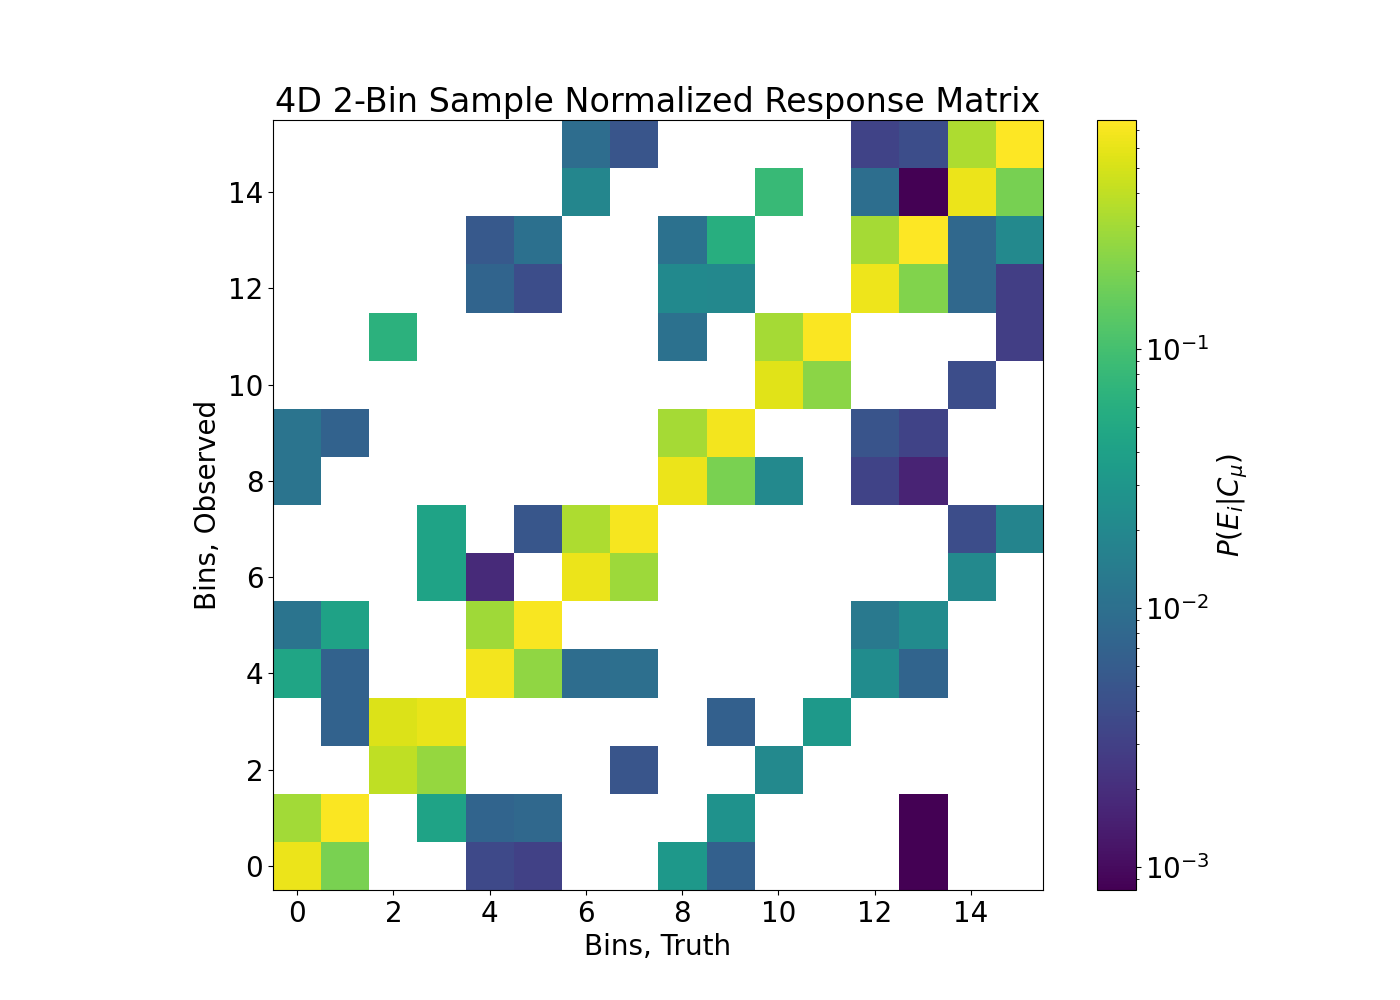
\includegraphics[width=0.449\textwidth]{Chapters/Ch5-Further/0_IBU/pics/4d-2n_example/4D_2bin_sample_normalized_response_matrix.png}
            \label{fig:ibu_toyc}}
            \hfill
            \subfloat[][Results of unfolding.]{
            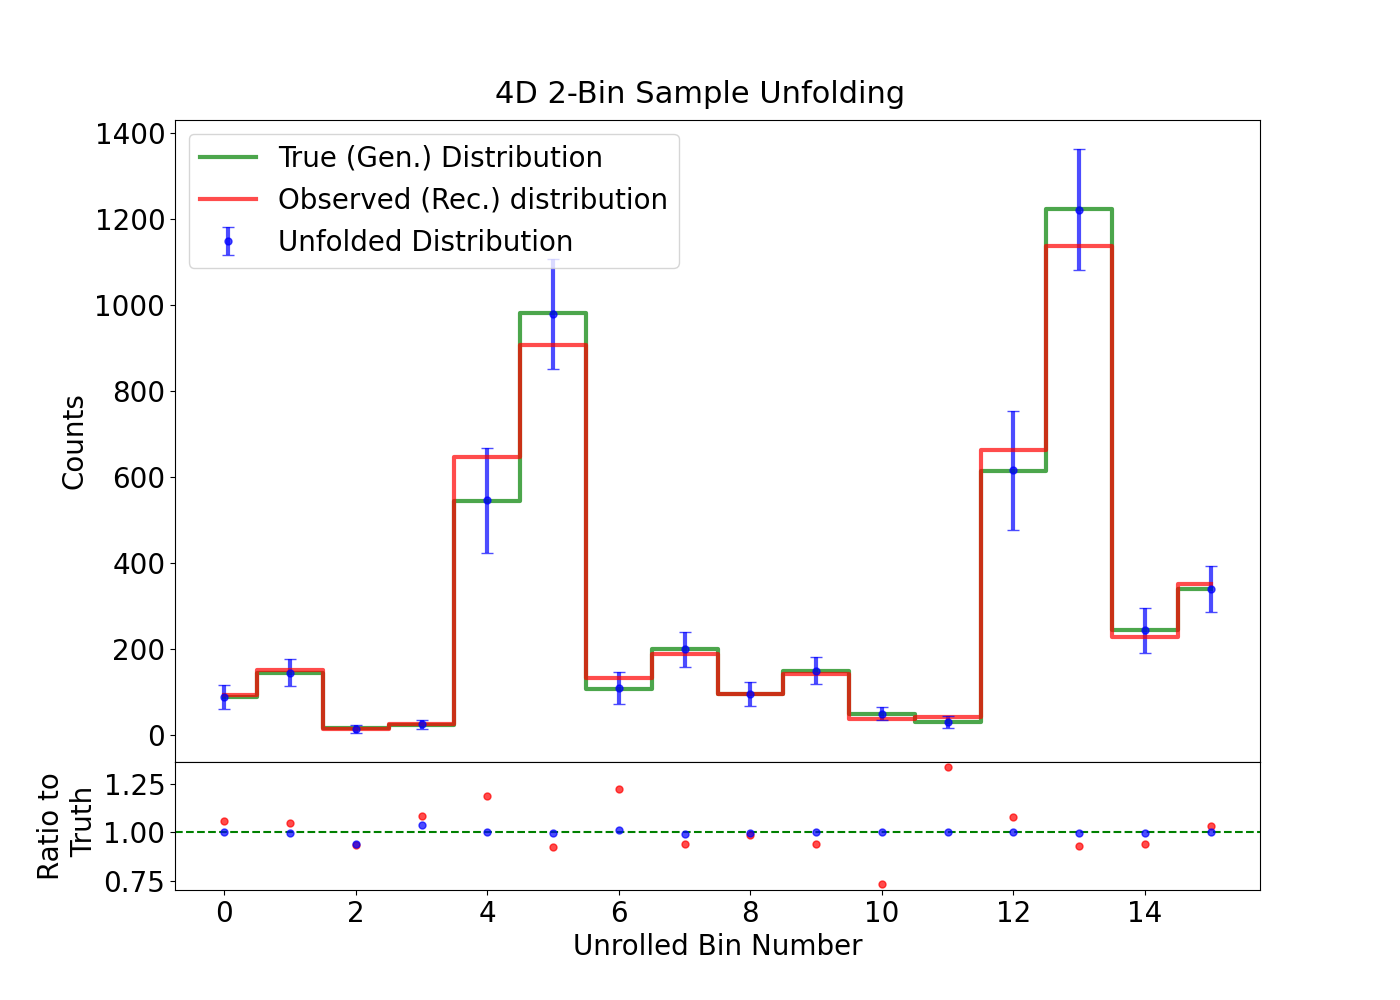
\includegraphics[width=0.449\textwidth]{Chapters/Ch5-Further/0_IBU/pics/4d-2n_example/4D_2bin_sample_unfolding.png}
            \label{fig:ibu_toyd}}
            \caption[2x2x2x2 IBU Result]{Sample calculation for 2x2x2x2 bin case. We can observe in (d) that the unfolding allows for a much closer truth estimate than the nominal observed data.}
            \label{fig:ibu_toy}
        \end{figure}


        2x2x2x2 is small enough to compute directly, without any kernel needed. A 4x4x4x4 bin group is the smallest that allows for verification of the 3x3x3x3 window method. \figref{fig:4x4unfold} shows the results of the complete unfolding analysis, processed with a 3$^4$ kernel. Again the unfolded results show close matching with the generated data distribution, demonstrating proper function of the unfolding and segmenting techniques.
    
        \begin{figure}[H]
            \centering
            \subfloat[Response matrix.]{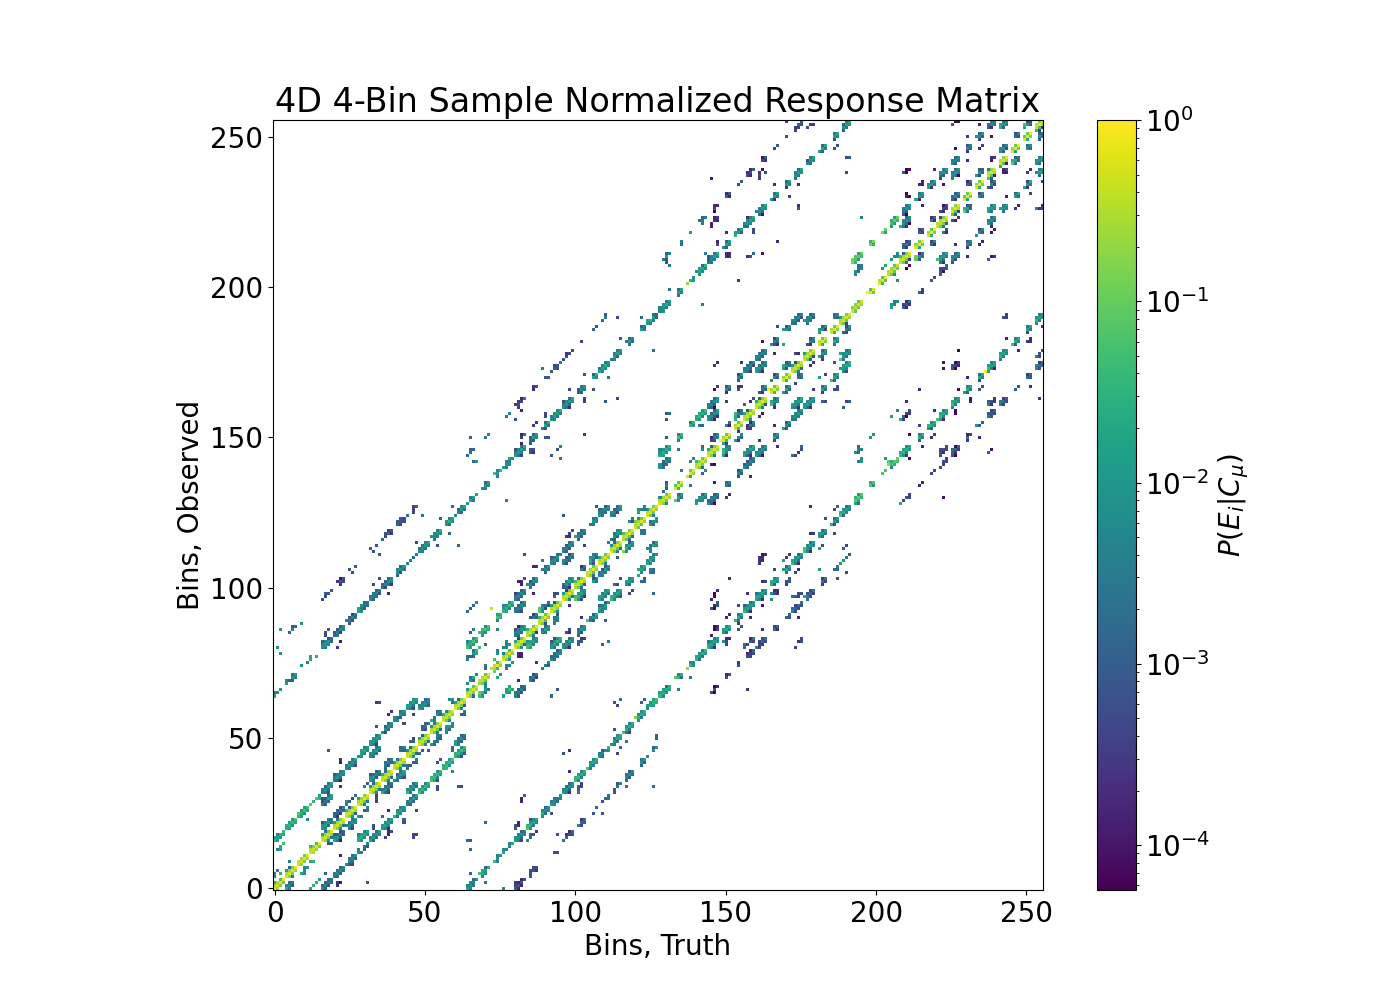
\includegraphics[trim={0 0 0 0},clip,width=0.5\textwidth]{Chapters/Ch5-Further/0_IBU/pics/4d-4n-3nkernel/4D_4bin_sample_normalized_response_matrix.png}}
            \subfloat[Results of unfolding.]{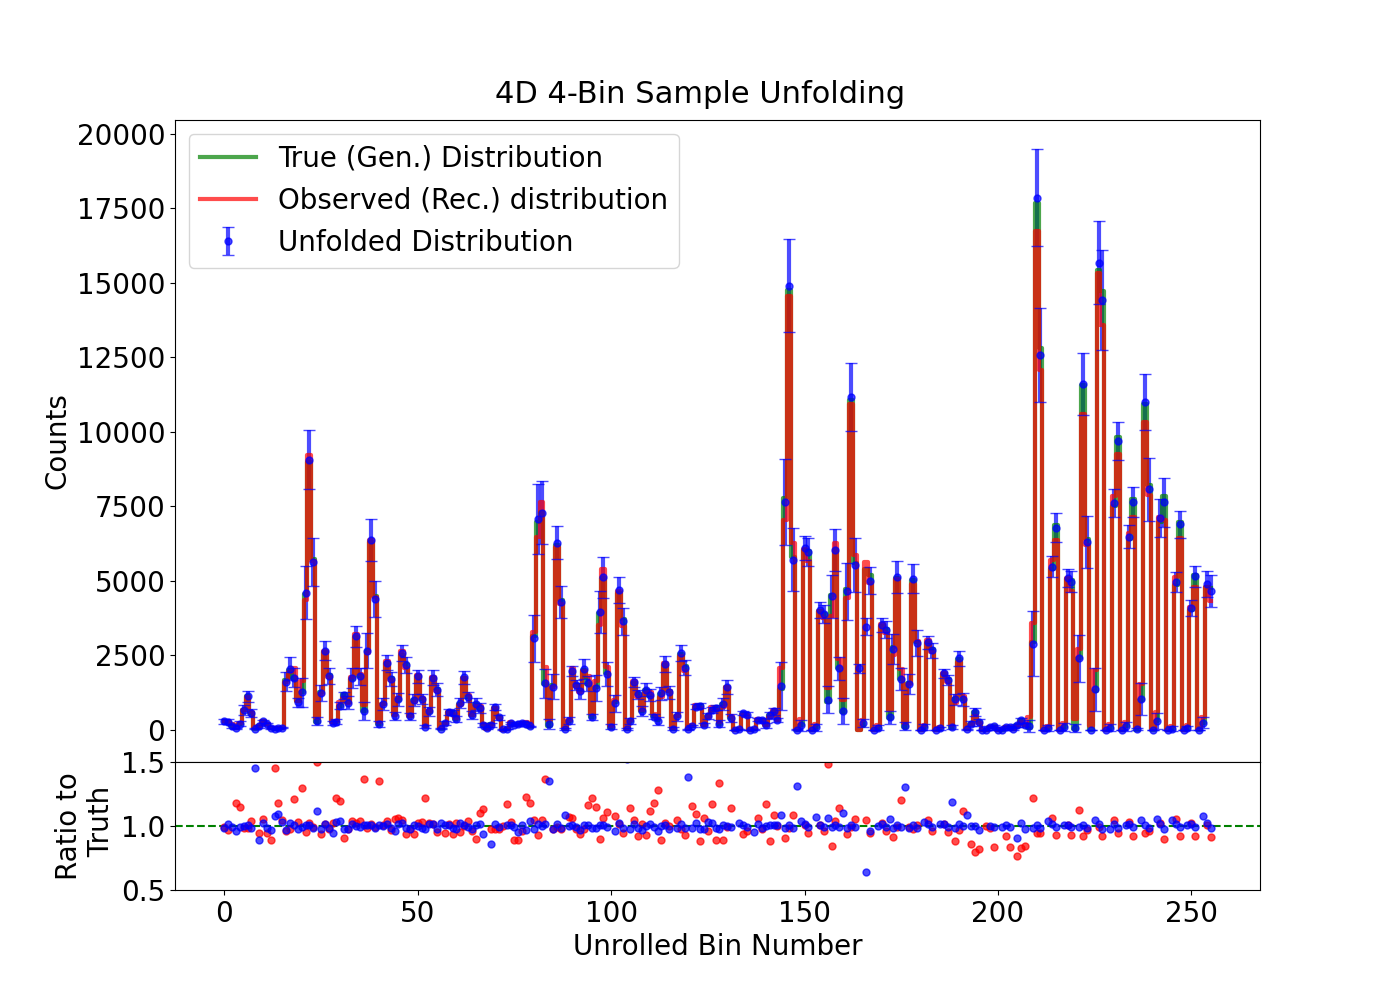
\includegraphics[trim={0 0 0 0},clip,width=0.5\textwidth]{Chapters/Ch5-Further/0_IBU/pics/4d-4n-3nkernel/4D_4bin_sample_unfolding.png}}
            \hfill
            \caption[4x4x4x4 IBU Result]{ Result for 4x4x4x4 grouping with 3$^4$ bin window.}\label{fig:4x4unfold}
        \end{figure}

        Finally, we can investigate the effect of computing the unfolding matrix via a kernel compared to the entire matrix by varying the kernel and stride size. This was performed for a 2D case as well as the more critical 4D case, with results summarized in \figref{fig:2d-4d-strider-kernel-comp}. Overall, we see that processing the unfolding matrix by taking a small kernel is much more computationally efficient, and yields approximately identical results provided the kernel is large enough and the stride is small enough. Also, we see that a kernel of $2^d$ leads to significant deviation compared to processing the full matrix at once, which makes sense considering a kernel of that size cannot capture all neighboring bins at the same time. Similarly, increasing stride length decreases the fidelity of the method. Accordingly, we are confident in scaling this approach to the full 6,400 bin scope of the analysis at hand. 
    
    \begin{figure}[ht]
        \centering
        \subfloat[2D Bin Unfolding with various kernels and strides.]{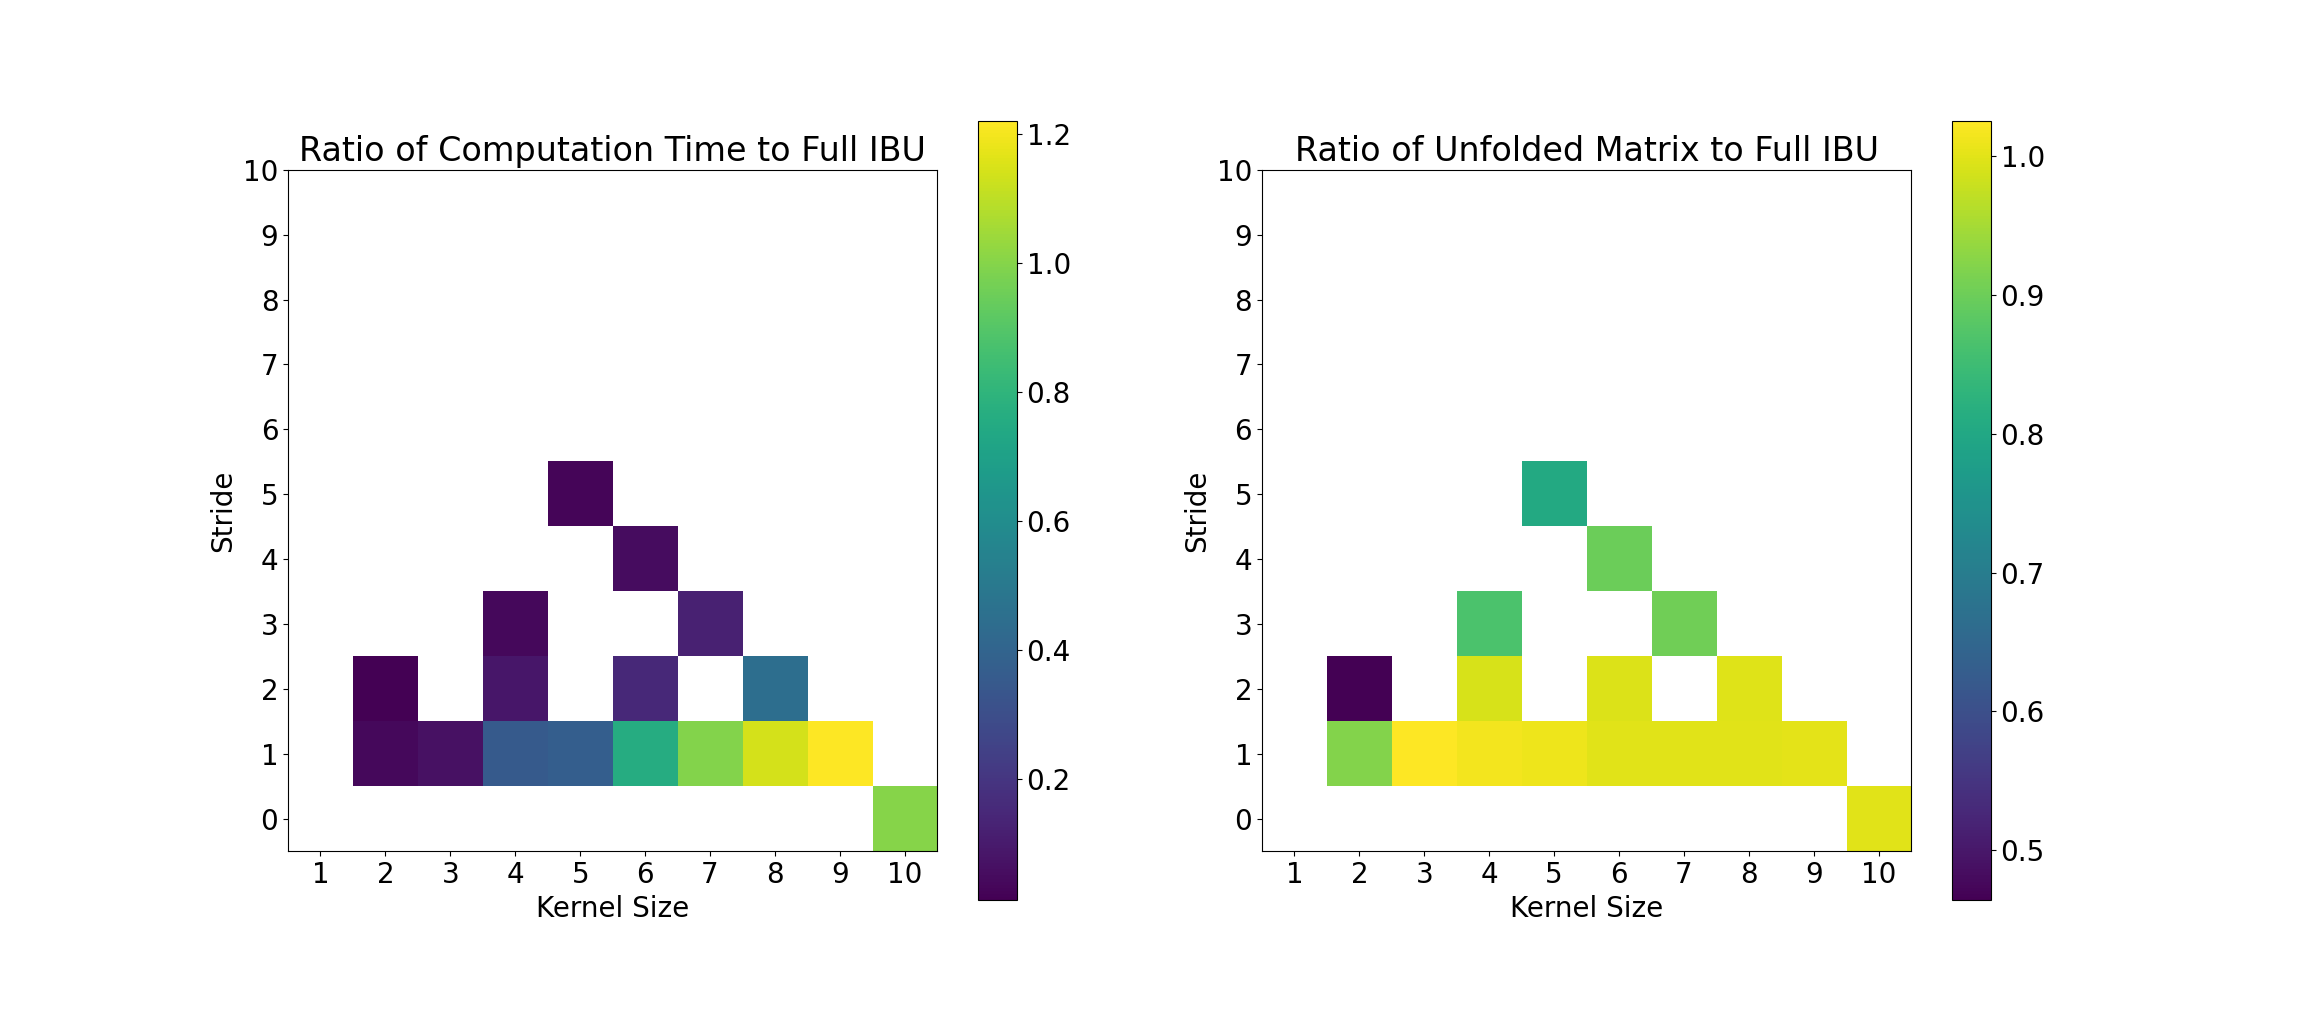
\includegraphics[trim={0 0 0 0},clip,width=\textwidth]{Chapters/Ch5-Further/0_IBU/pics/stride_2D.png}\label{fig:ibu_stride_2D}}
    
        \subfloat[4D Bin Unfolding with various kernels and strides.]{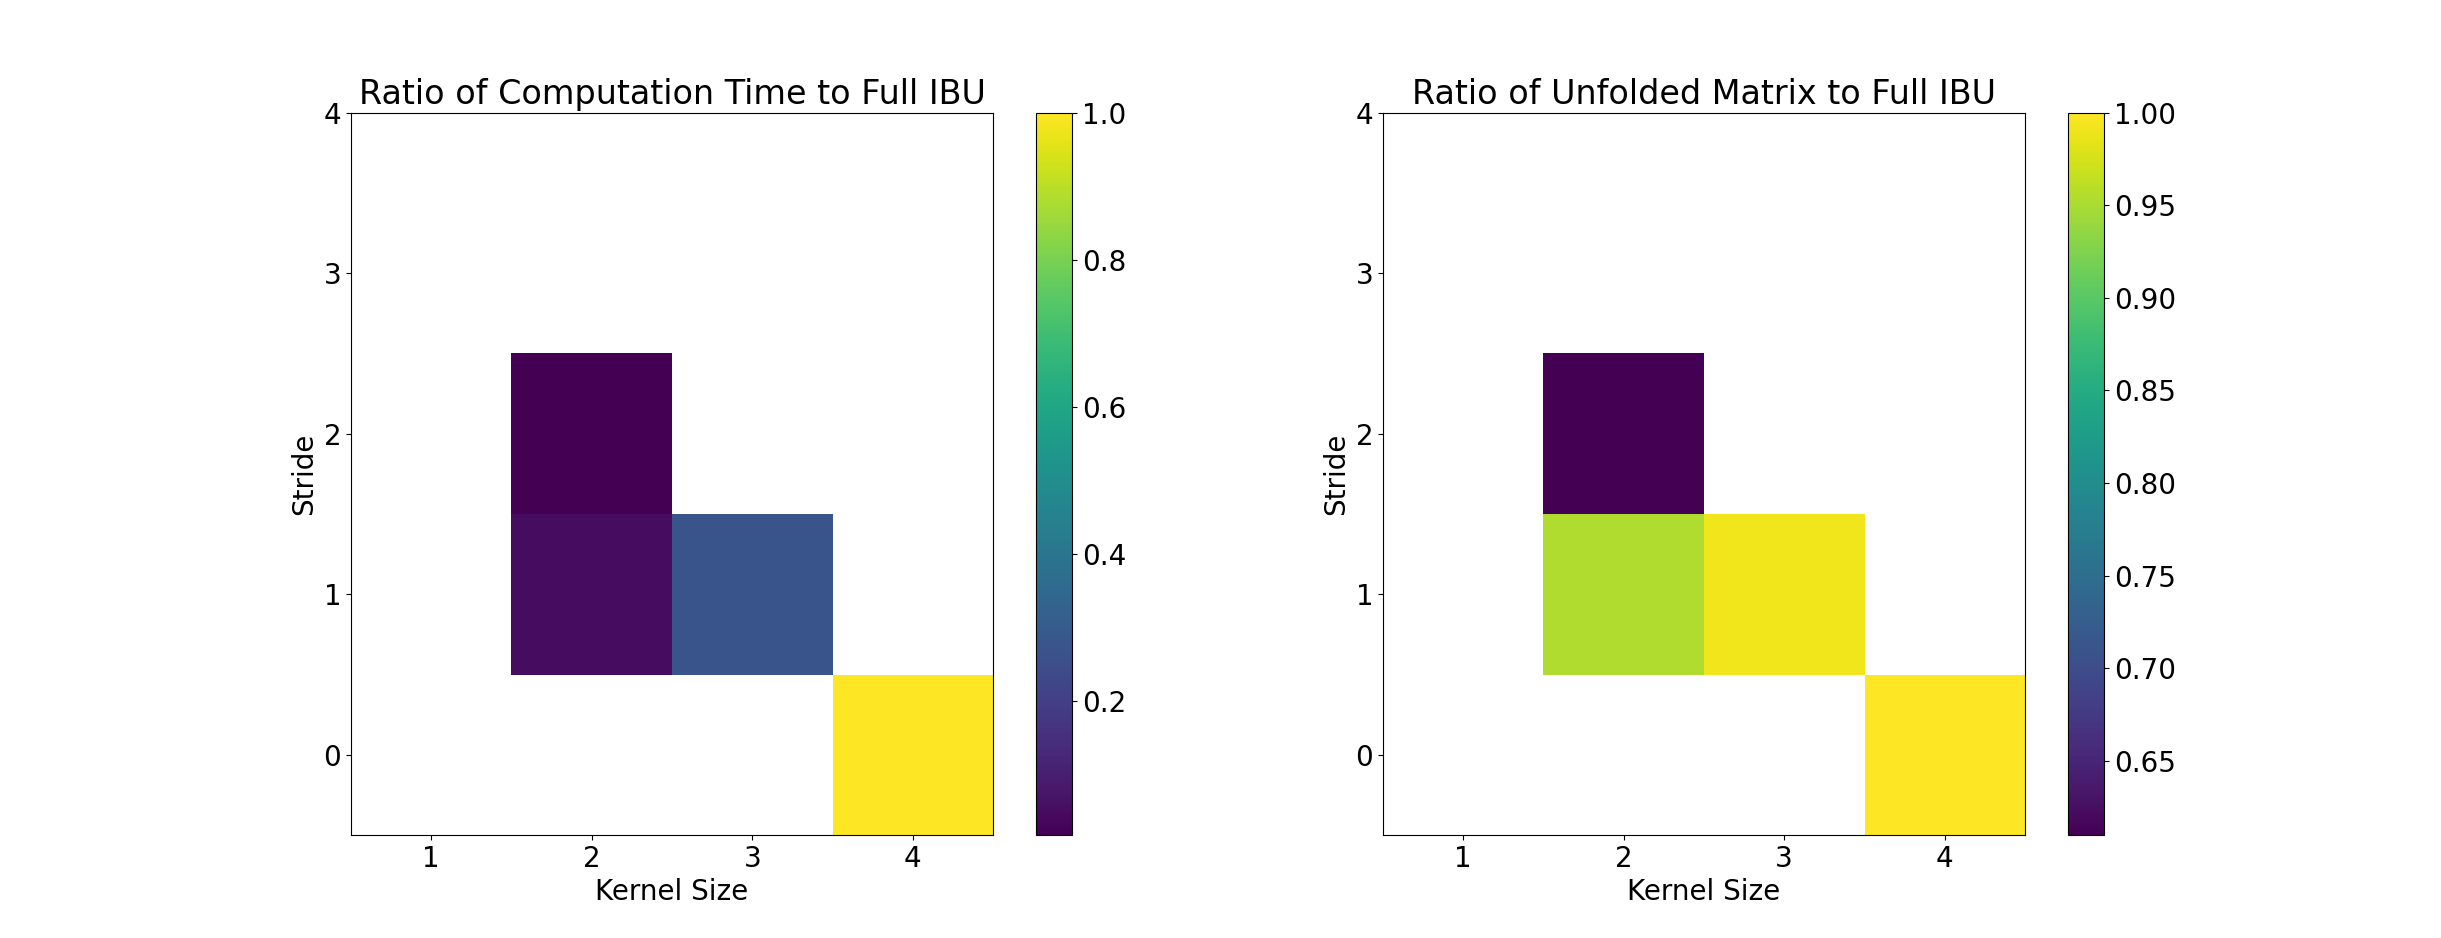
\includegraphics[trim={0 0 0 0},clip,width=\textwidth]{Chapters/Ch5-Further/0_IBU/pics/stride_4D.png}\label{fig:ibu_stride_4D}}
    
        \caption[Kernel and Stride Dependence of IBU]{Dependence of IBU calculation time (left) and unfolding matrix results (right) on kernel size (horizontal axis) and stride length (vertical axis) for two (top) and four (bottom) dimensions. As long as the kernel is large enough to capture all $3^d$-1 neighboring bins in d-dimensions and the stride is small enough to allow kernel overlaps, the results of the unfolding matrix are similar between all kernel choices. Only combinations of kernels and strides leading to full tessellation of the binning space were calculated. }
        \label{fig:2d-4d-strider-kernel-comp}
    \end{figure}

    
    \clearpage
\section{Results of Unfolding}

    \subsection{Unfolded Matrix Results}
       

        \iffalse
        \begin{figure}[ht]
            \centering
            \subfloat[]{
                \begin{tikzpicture}
                    \node[anchor=south west,inner sep=0] (image) at (0,0) {
                        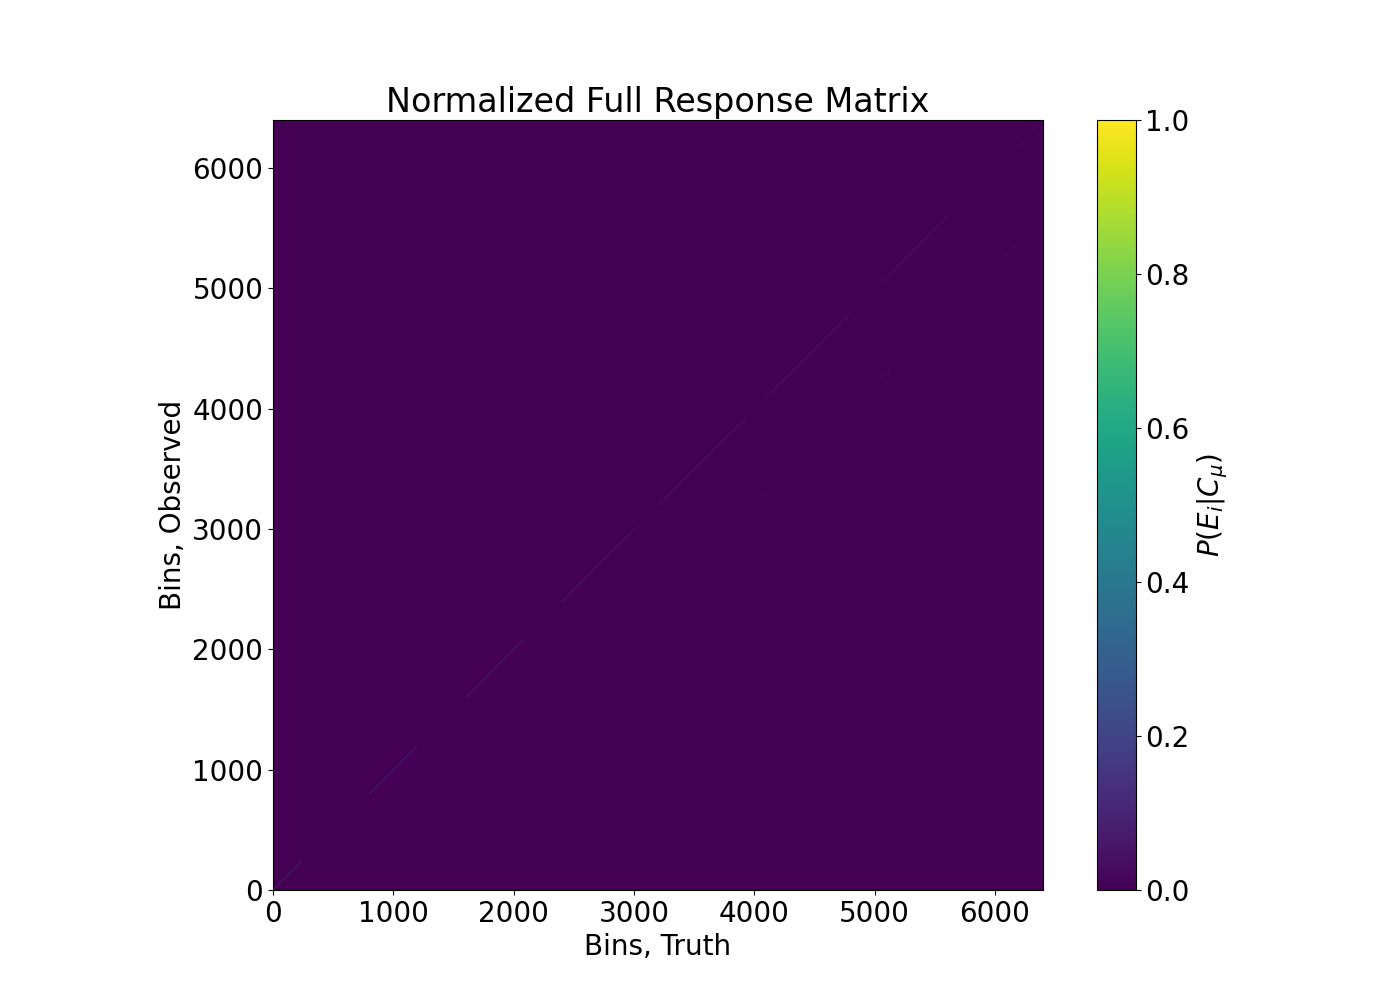
\includegraphics[trim={0 0 0 0},clip,width=0.45\textwidth]{Chapters/Ch5-Further/0_IBU/pics/4D_all_bins_normalized_full_response_matrix.png}
                    };
                    \begin{scope}[x={(image.south east)},y={(image.north west)}]
                        \draw[red,ultra thick] (0.43,0.45) rectangle ++(0.1,0.1.5); %Change the values as per your need
                    \end{scope}
                \end{tikzpicture}
                \label{fig:ibu1}
            }
            \hfill
            \subfloat[]{
                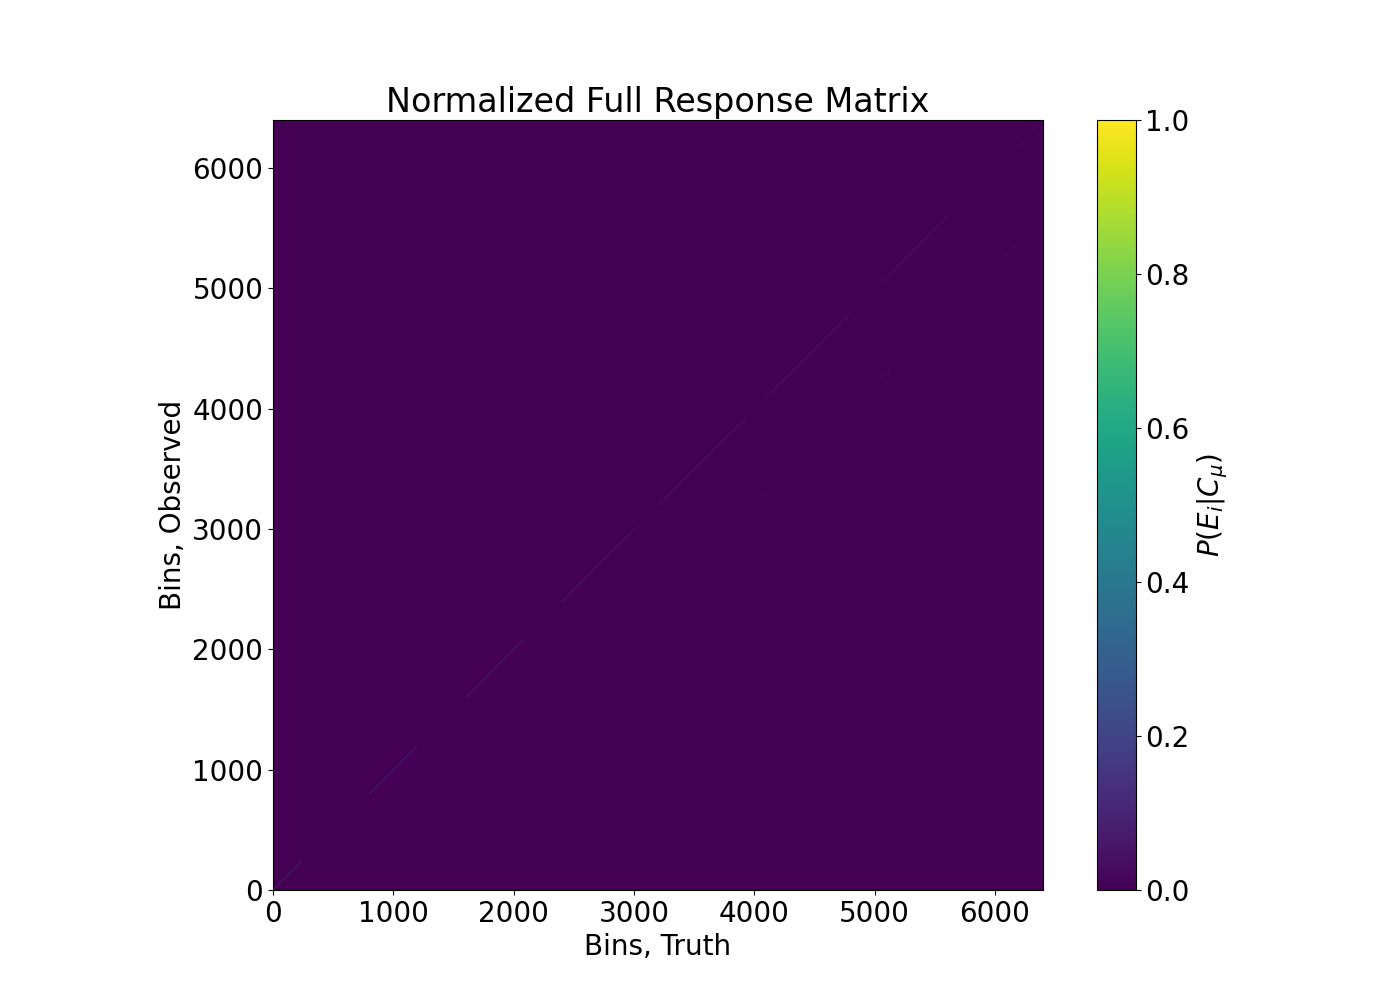
\includegraphics[trim={16cm 12cm 17cm 11cm},clip,width=0.4\textwidth]{Chapters/Ch5-Further/0_IBU/pics/4D_all_bins_normalized_full_response_matrix.png}
                \label{fig:ibu2}
            }
            \caption{Caption for both figures}
            \label{fig:ibu}
        \end{figure}
        \fi

    Processing was performed locally, taking approximately a day to run on a single core machine. Parallelization is possible but was not explored. \figref{fig:ibufullresult} shows the bin-by-bin comparision of truth, observed, and unfolded values, but it is somewhat difficult to inspect the results at this scope. \figref{fig:residualsIBU} provides more informative comparisons of the raw observed data and the data after unfolding.  Unfolding does not yield perfect results, but on average we have significantly decreased the distance to the true number of events in any given bin.

    \begin{figure}[H]
        \centering
        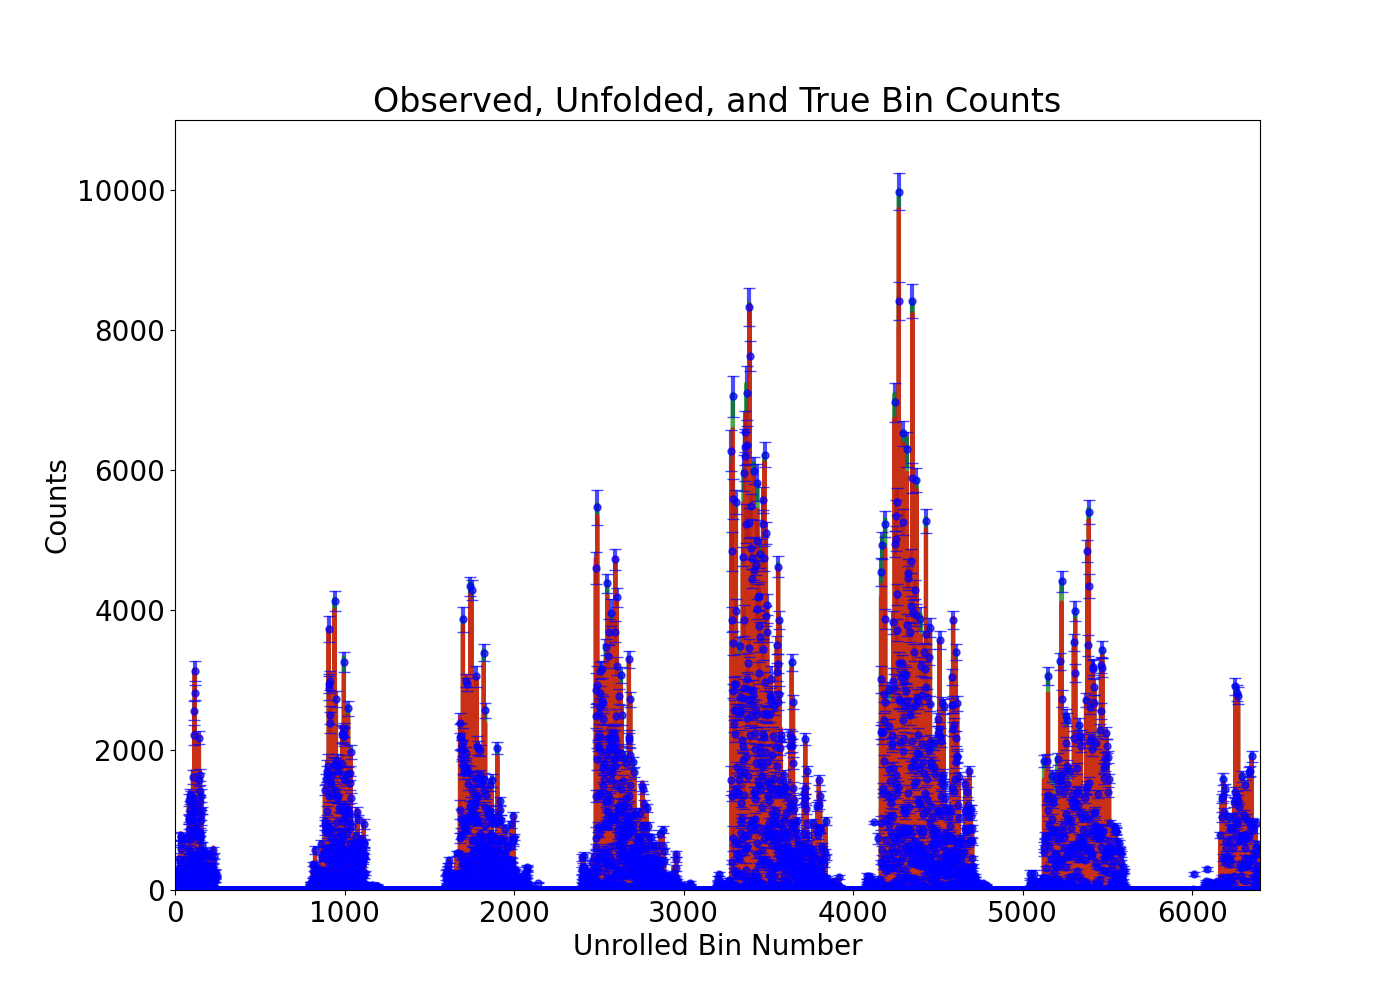
\includegraphics[trim={0 0 0 0},clip,width=0.8\textwidth]{Chapters/Ch5-Further/0_IBU/pics/complete/final_observed_unfolded_and_true_bin_counts.png}
        \caption[Comparison of Truth, Observed, and Unfolded Distributions]{Comparison of true (green) observed (red) and unfolded (blue) event counts across all bins for this analysis. Error bars combine statistical (counting) and systematic (from the unfolding procedure) errors in quadrature.}
        \label{fig:ibufullresult}
    \end{figure}


    \begin{figure}[ht]
        \centering
        \subfloat[Ratio to truth.]{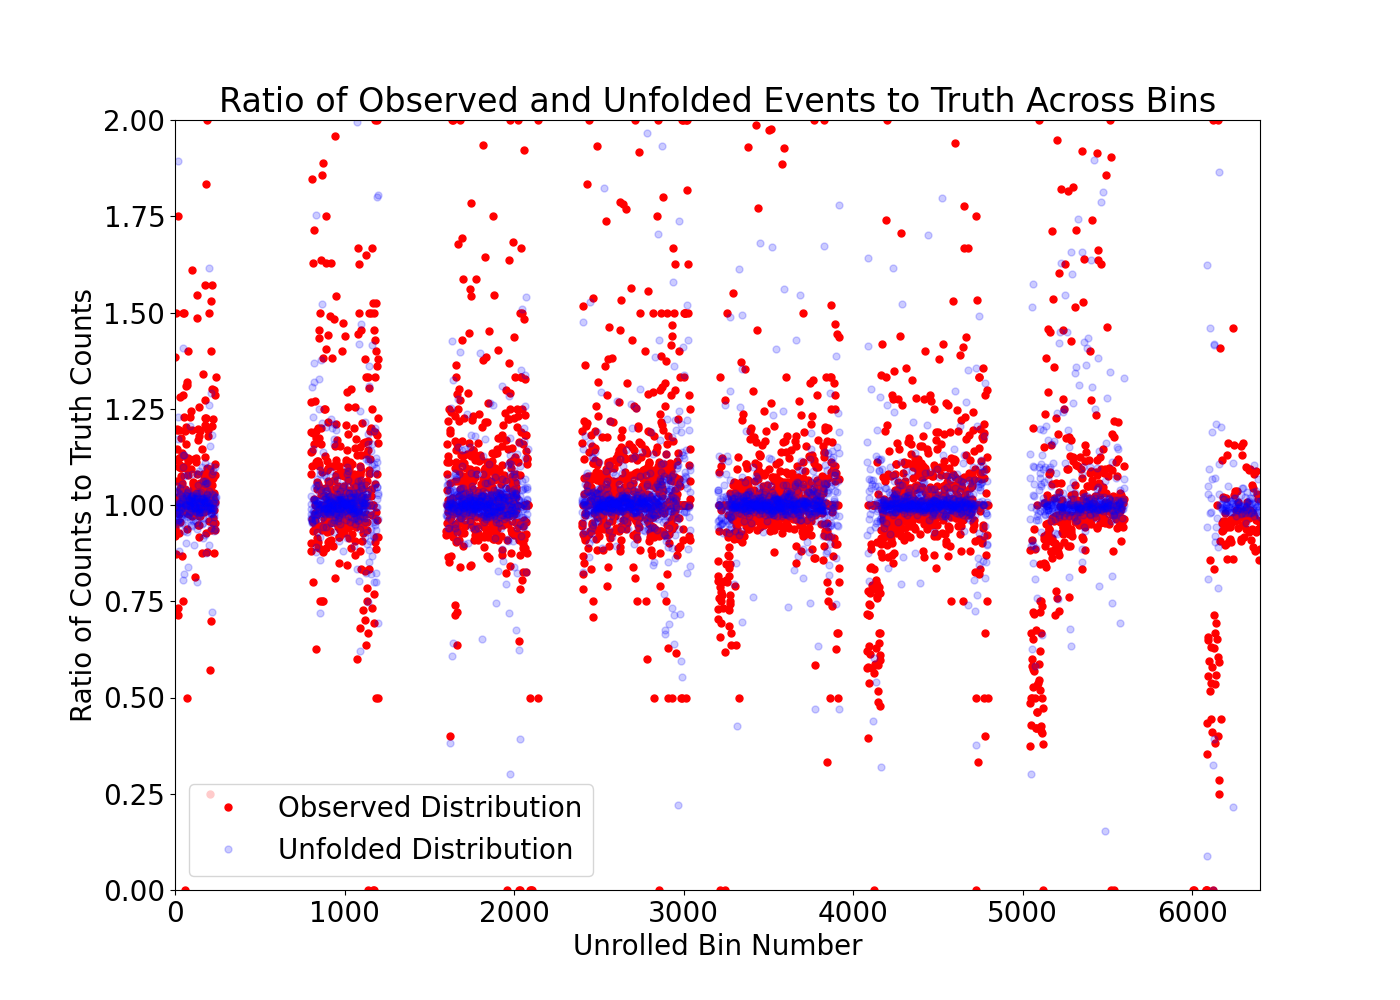
\includegraphics[trim={0 0 0 0},clip,width=0.48\textwidth]{Chapters/Ch5-Further/0_IBU/pics/complete/ratio_of_observed_and_unfolded_events_to_truth_across_bins.png}\label{fig:ibu3}}
        \subfloat[Histogram of ratio to truth.]{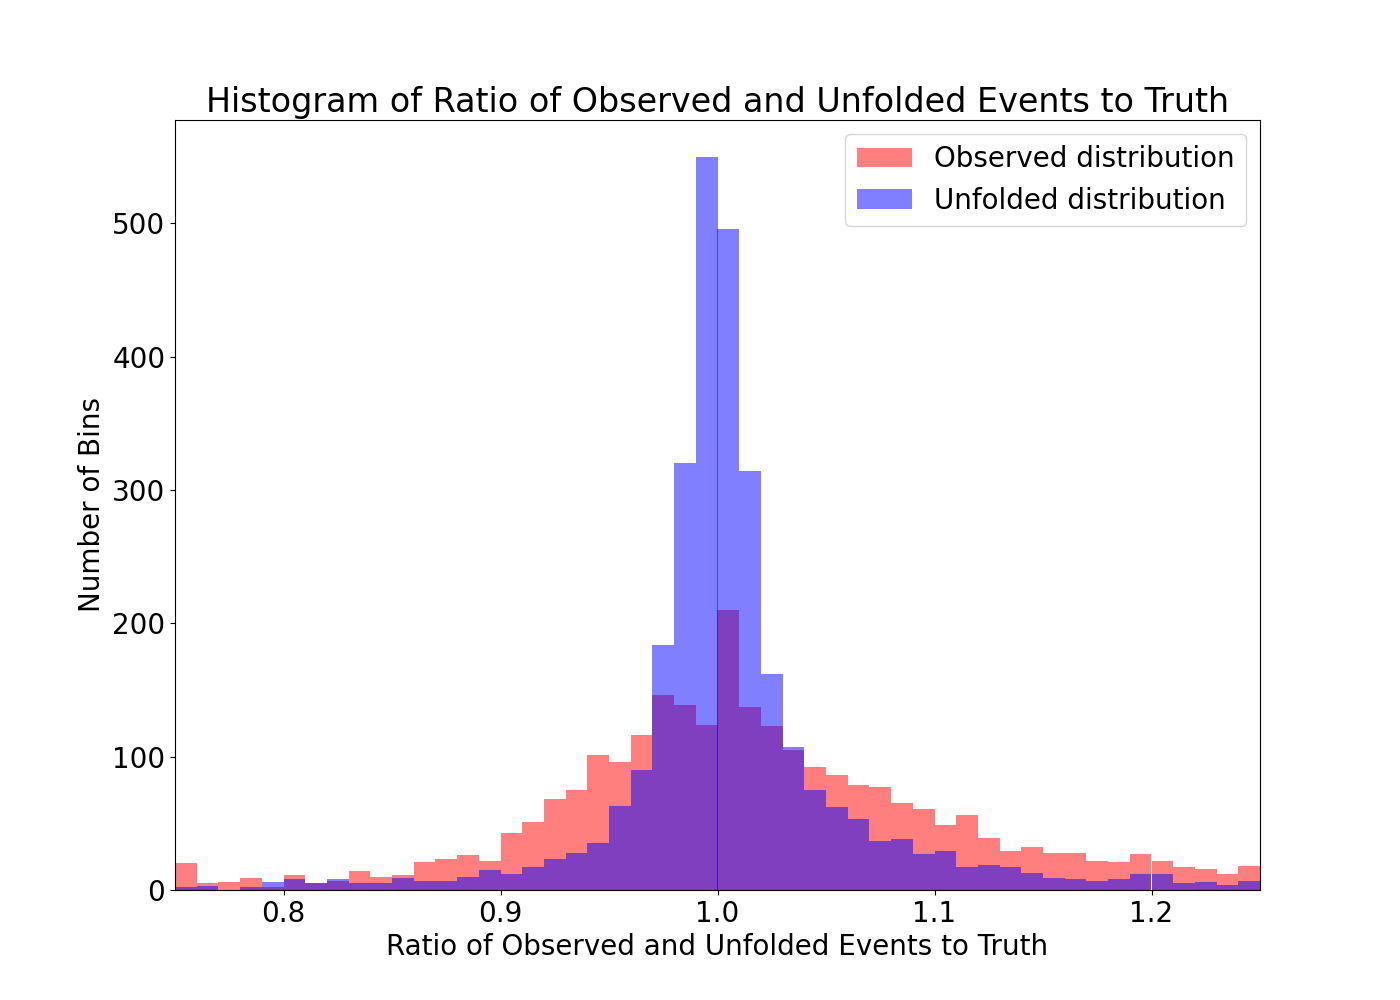
\includegraphics[trim={0 0 0 0},clip,width=0.48\textwidth]{Chapters/Ch5-Further/0_IBU/pics/complete/histogram_of_ratio_of_observed_and_unfolded_events_to_truth.png}\label{fig:ibu1}}
        \caption[Full Unfolding Residuals]{Ratio of observed and unfolded event distribution to truth (a) and histogram of those ratios (b). We observe the unfolded distribution (blue) is significantly closer to the generated one than the observed data before unfolding is applied.}
        \label{fig:residualsIBU}
    \end{figure}
    

    \clearpage
    \subsection{Unfolding Effect on Cross Section Values}
    The cross section was calculated using the calculated unfolding matrix and compared to the bin-by-bin result which neglected bin migrations. \figref{fig:binbybinIBU} shows a comparison of these two results for sample datapoints; full cross sections results for both bin-by-bin methods and unfolding are shown in the following chapter. \figref{fig:ibufullresult2} summarizes the effect of unfolding as a ratio of the cross section result between these two methods; the mean difference in value is 15\%.
     

    \begin{figure}[H]
        \centering
        \subfloat{
        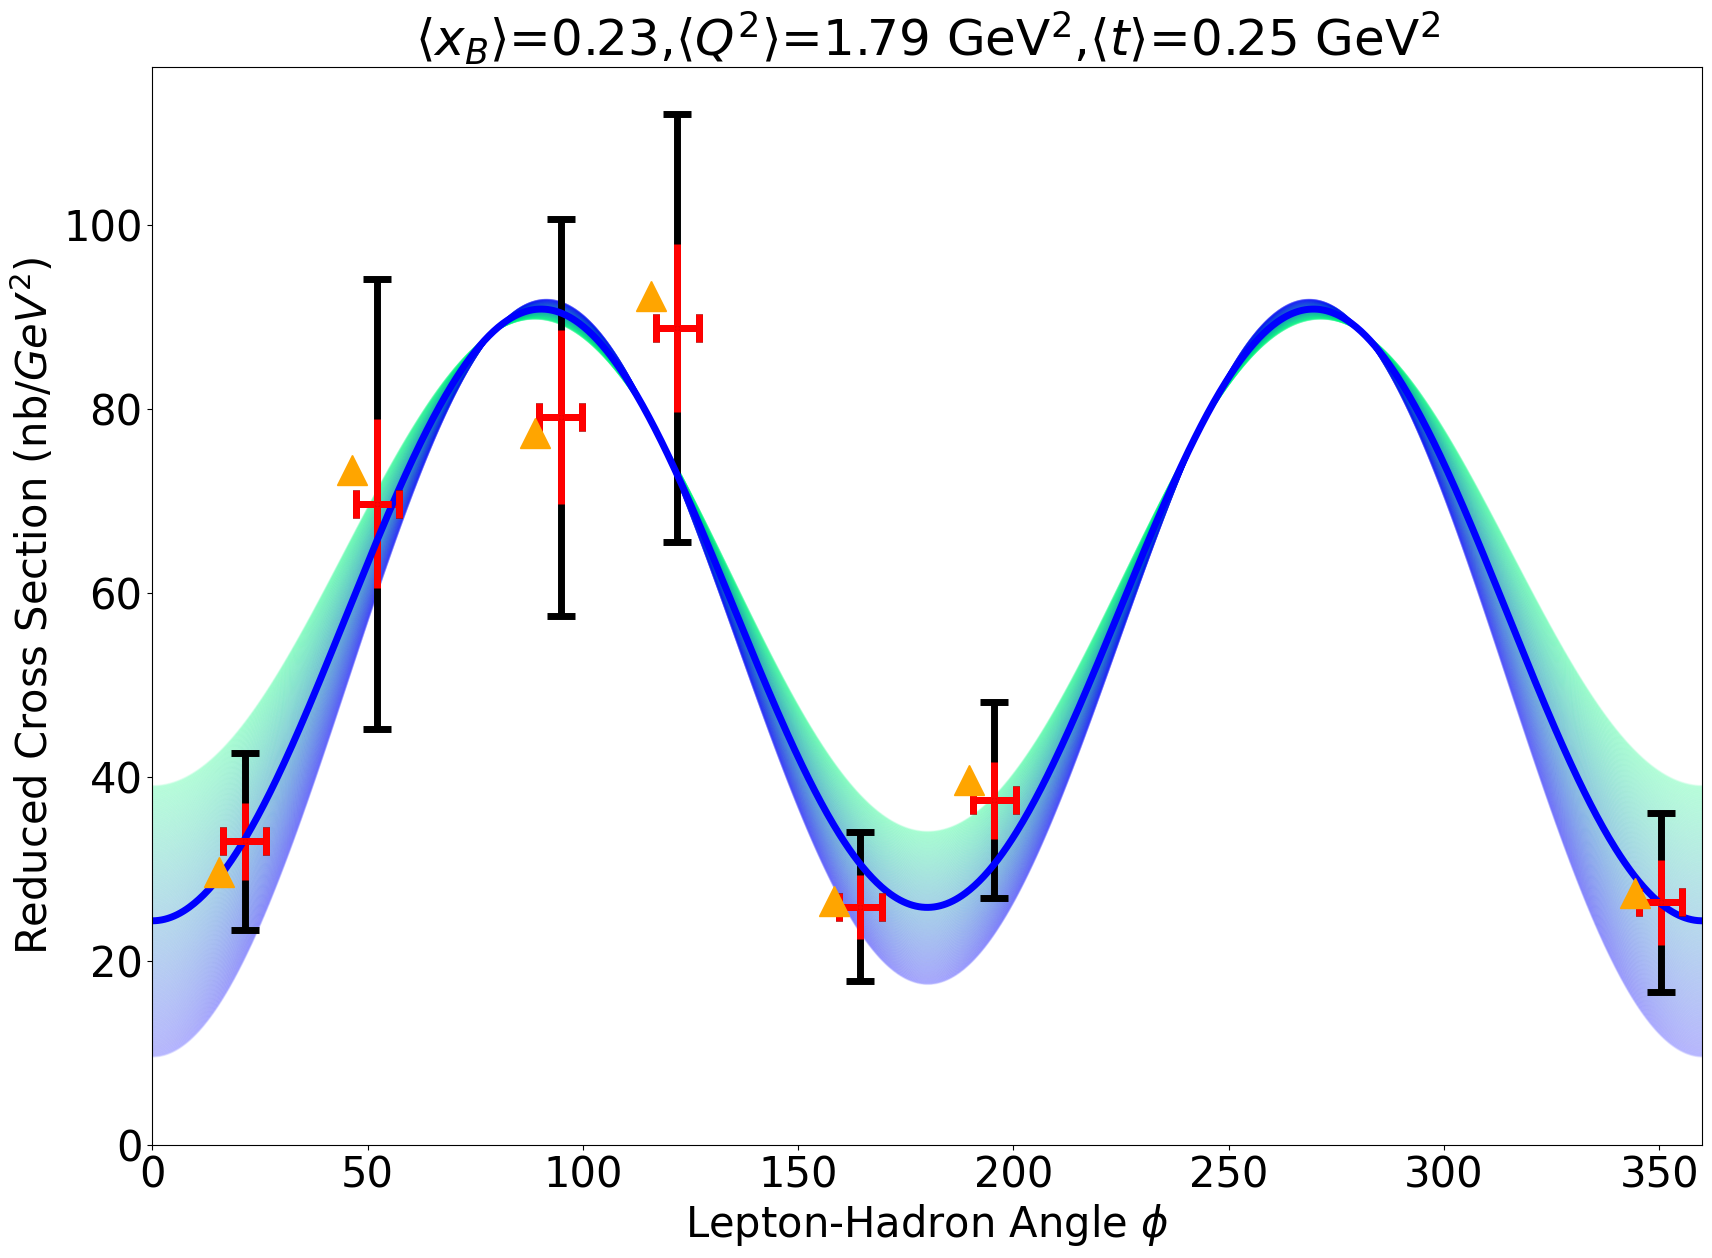
\includegraphics[width=0.45\textwidth]{Chapters/Ch5-Further/0_IBU/pics/xqt=(0.2, 1.5, 0.2).png}
        \label{fig:xa}
    }
            \subfloat{
        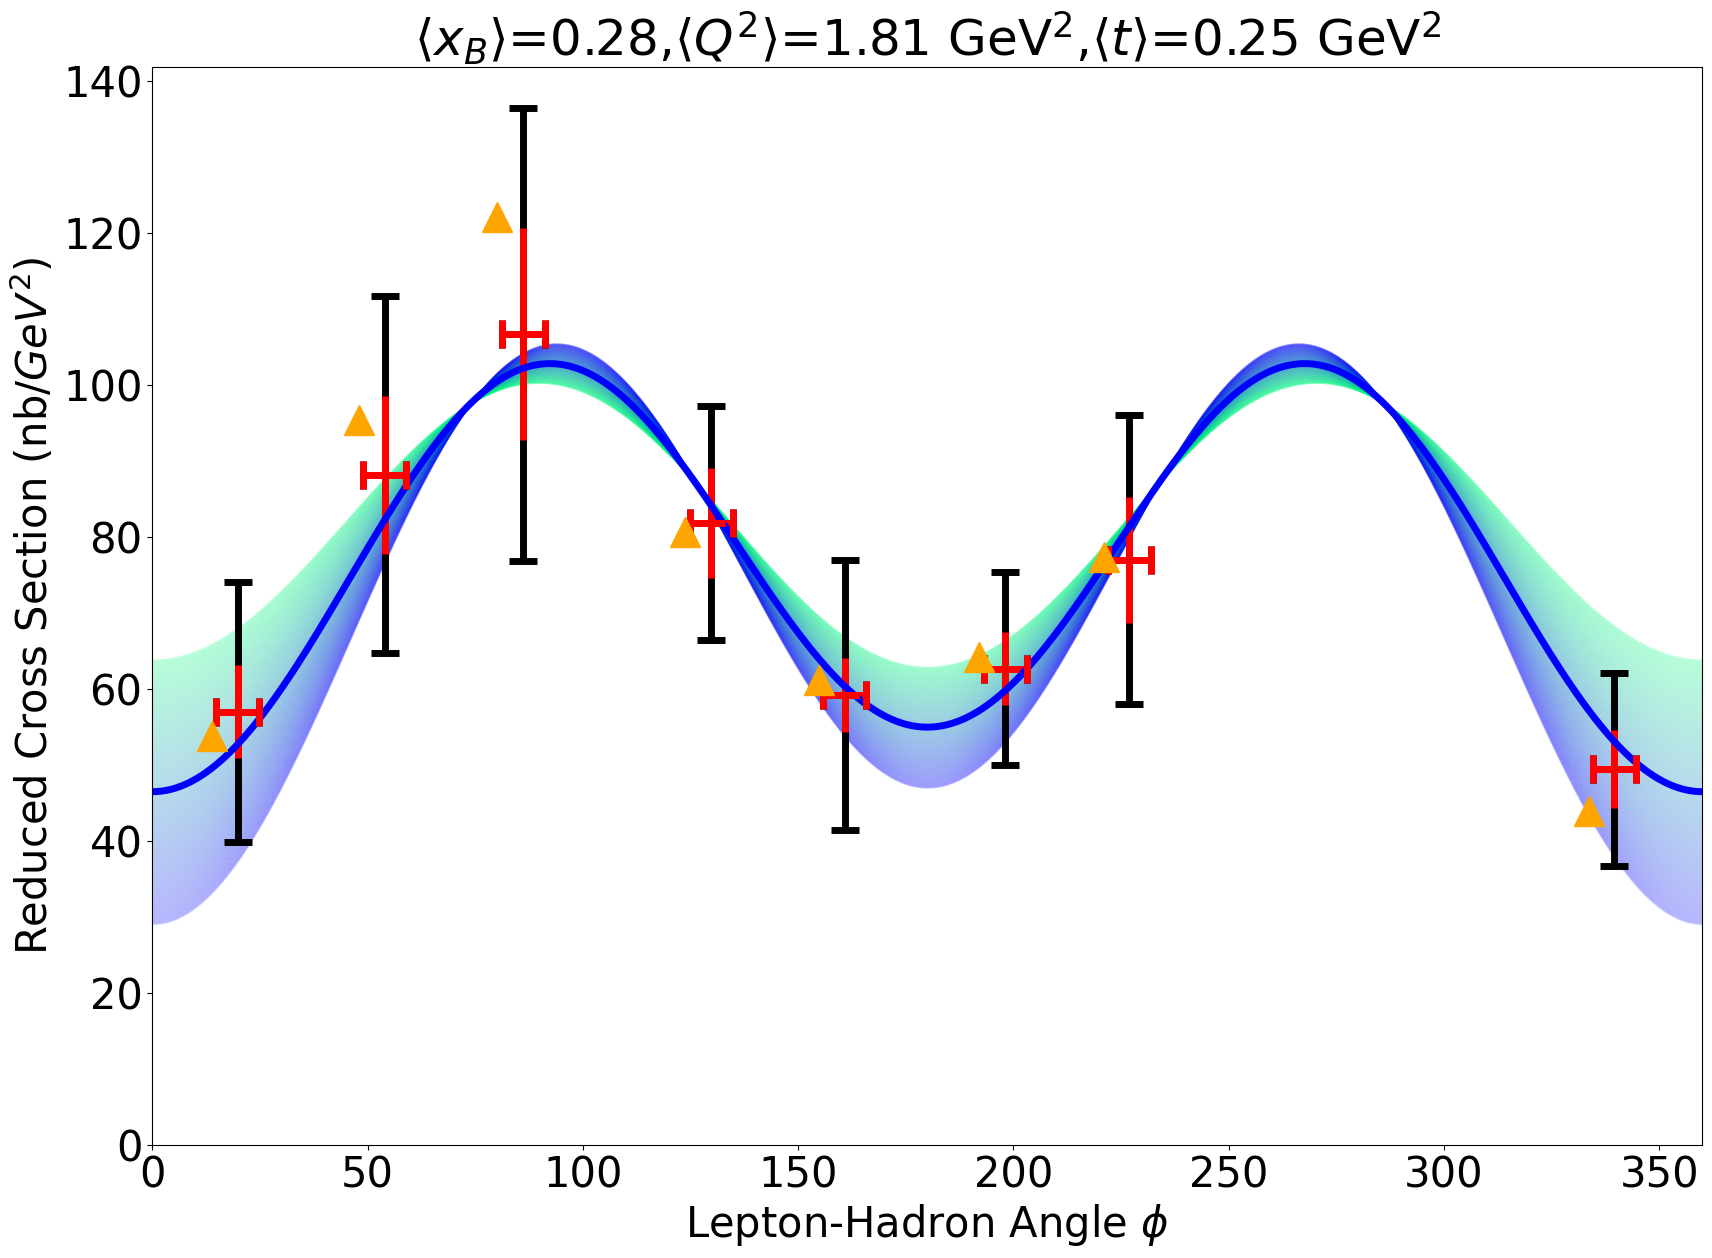
\includegraphics[width=0.45\textwidth]{Chapters/Ch5-Further/0_IBU/pics/xqt=(0.25, 1.5, 0.2).png}
        \label{fig:xb}
    } 
    \caption[Bin-by-bin and Unfolded Cross Section Examples]{Sample datapoints comparing bin-by-bin (orange triangle, offset to the left) and unfolding (red cross) results. Many bins have similar results, while some show shifts at the 10-20\% level. Vertical errors on the unfolded result are red (statistical only) and black (statistical and all systematic added in quadrature), errors are not shown on the bin-by-bin datapoints. The curve is an A+B$\cos{\phi}$+C$\cos{2\phi}$ fit, with a color gradient errorband that corresponding to the fit with high (light green) and low (dark blue) bounds of the fit error.}\label{fig:binbybinIBU}
    \end{figure}

    
    \begin{figure}[H]
        \centering
        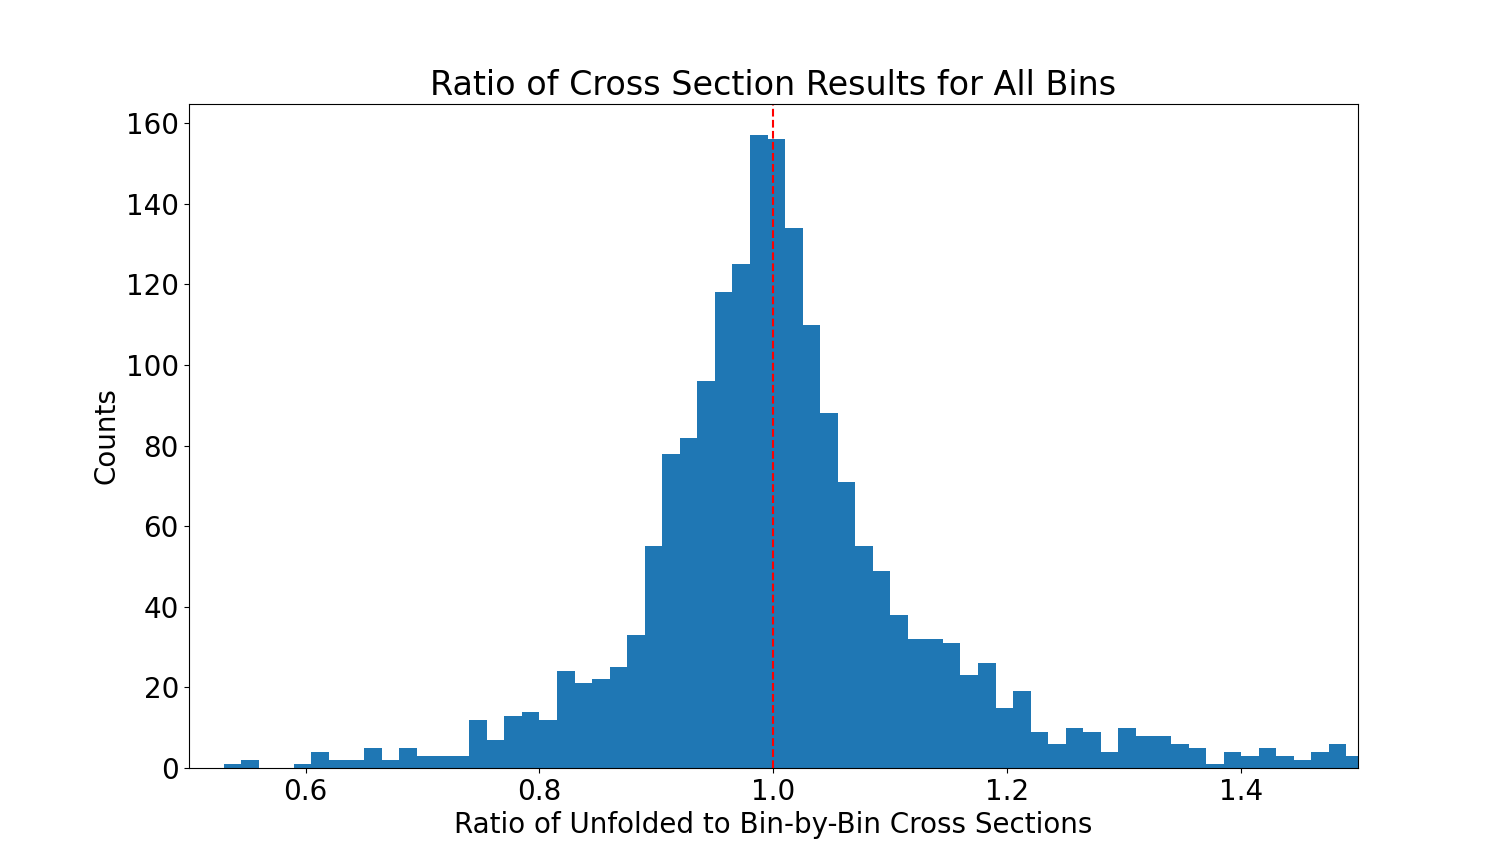
\includegraphics[trim={0 0 0 0},clip,width=0.8\textwidth]{Chapters/Ch5-Further/0_IBU/pics/results/binbybin_to_unfolded.png}
        \caption[Summary of Bin-by-Bin vs. Unfolded Cross Sections]{The ratio of cross section values obtained by bin-by-bin analysis compared to the results from the unfolding methods discussed in this chapter.}
        \label{fig:ibufullresult2}
    \end{figure}

\iffalse
    \begin{figure}[ht]
    \centering
    \subfloat[][]{
        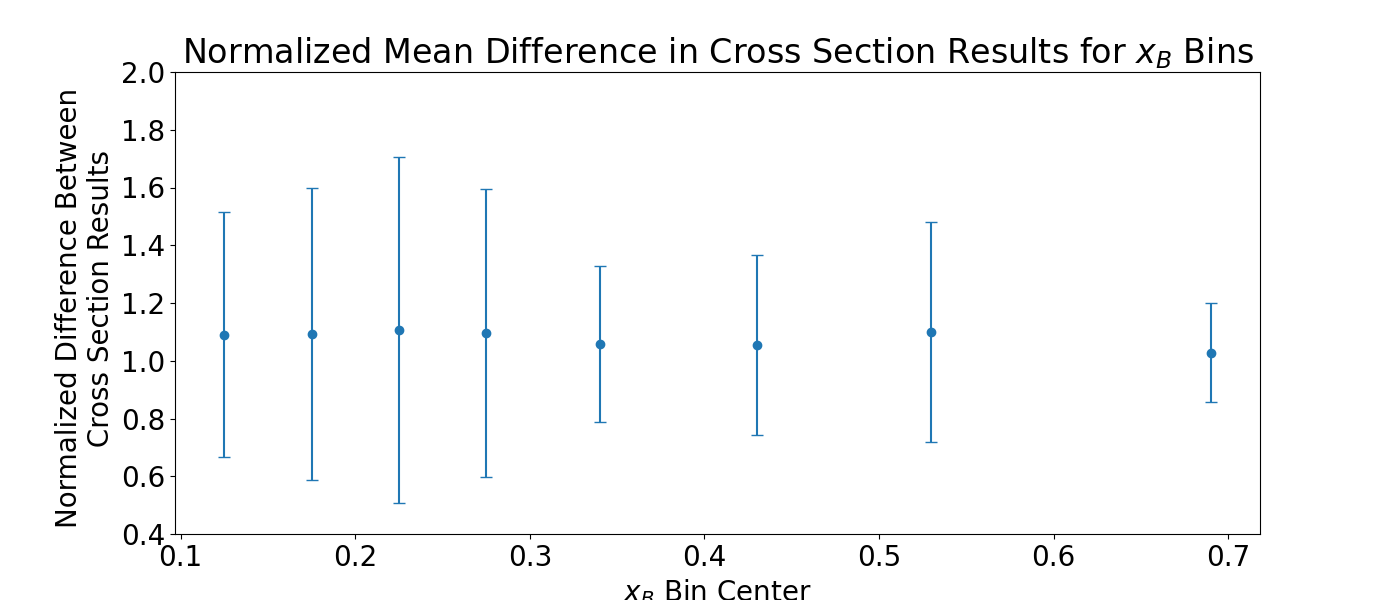
\includegraphics[width=0.45\textwidth]{Chapters/Ch5-Further/0_IBU/pics/folding_ratio_x.png}
        \label{fig:x}
    }
    \hfill
    \subfloat[][]{
        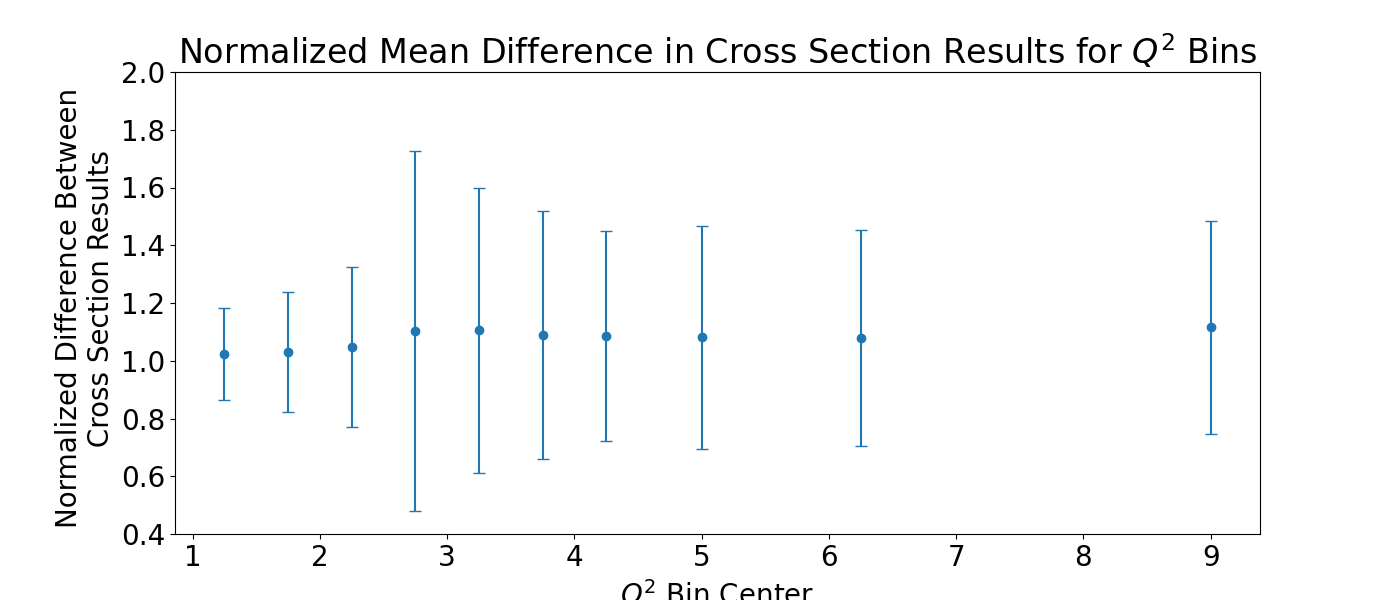
\includegraphics[width=0.45\textwidth]{Chapters/Ch5-Further/0_IBU/pics/folding_ratio_q.png}
        \label{fig:q}
    }
    \\
    \subfloat[][]{
        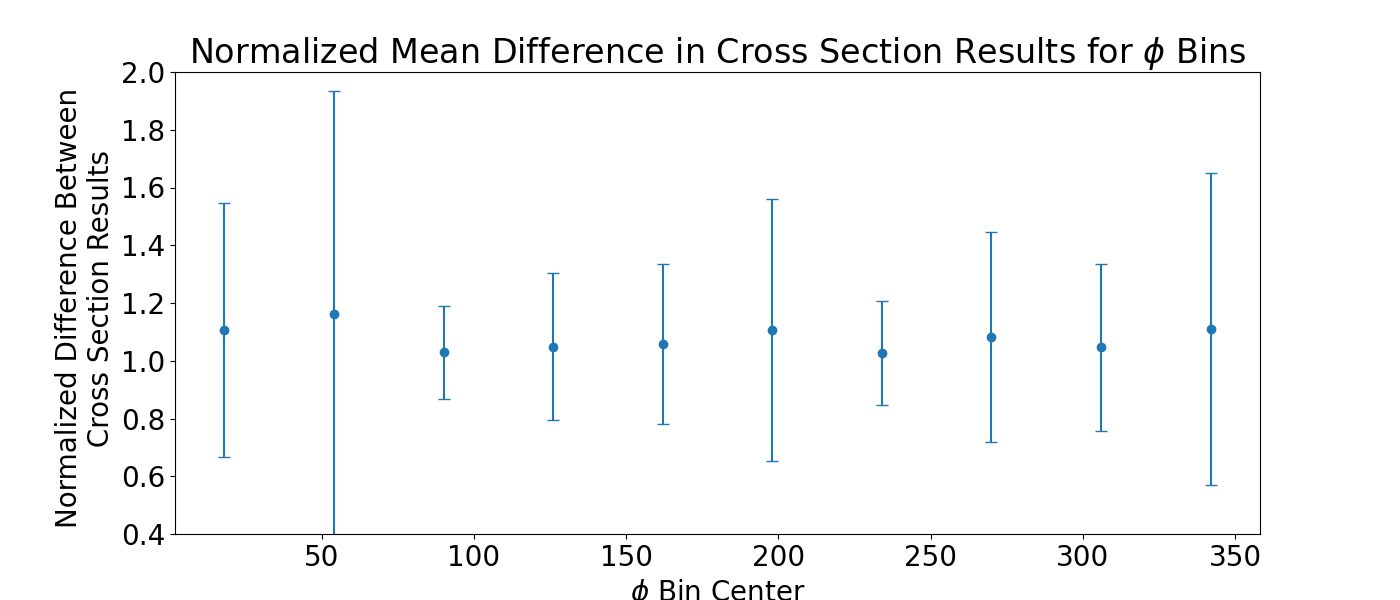
\includegraphics[width=0.45\textwidth]{Chapters/Ch5-Further/0_IBU/pics/folding_ratio_p.png}
        \label{fig:p}
    }
    \hfill
    \subfloat[][]{
        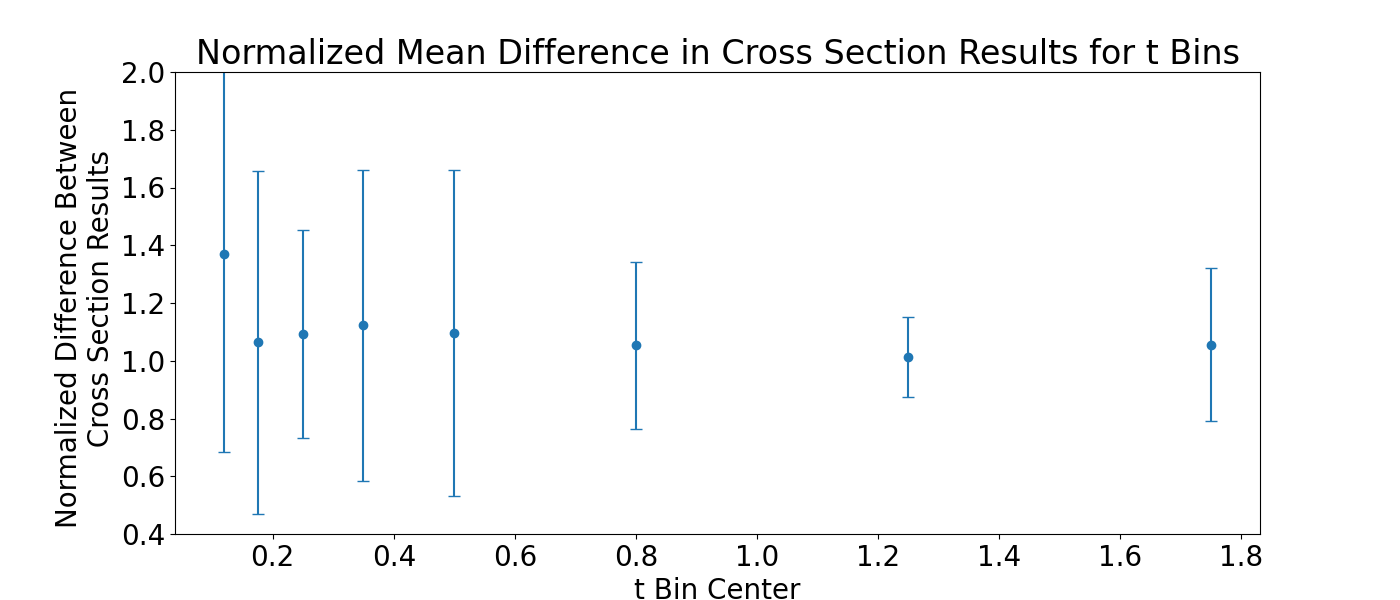
\includegraphics[width=0.45\textwidth]{Chapters/Ch5-Further/0_IBU/pics/folding_ratio_t.png}
        \label{fig:t}
    }
    \caption{Folding Ratio Plots}
    \label{fig:folding_ratios}
\end{figure}
\fi